%========= Mémoire de Projet de Fin d'Études ==============%
% HelpDesk AI — Mohamed Amine TOUKABRI                     %
% Template TEK-UP (isipfe) — sept chapitres
%==========================================================%

\documentclass[]{./tpl/isipfe}
\graphicspath{{./img/}}

%============ Compatibilite listes / babel-french ========%
% babel-french (french3.ldf) redefinit itemize, enumerate et description,
% ce qui entre en conflit avec enumitem charge par la classe : toute liste
% declenche une cascade « Undefined control sequence \enit@after ».
% StandardLists rend la main a enumitem. L'appel doit precederi
% \selectlanguage{french}, effectue dans tpl/new_commands.tex.
\frenchsetup{StandardLists=true}

%============= Placement des flottants ====================%
% \FloatBarrier force la sortie des tableaux et figures en attente avant de
% poursuivre. Sans lui, un tableau trop haut pour tenir en fin de page est
% reporte au sommet de la suivante et se retrouve apres le debut de la section
% qui suit, donc detache du texte qui l'annonce.
% Les tableaux de plus d'une page se paginent au lieu de deborder.
\usepackage{longtable}
\usepackage{placeins}

% Un titre de section suivi de deux ou trois lignes, puis une rupture de page :
% le lecteur tourne la page pour trouver la premiere sous-section, et le titre
% reste seul en bas. \Needspace reserve la place avant d'ecrire le titre, et
% reporte l'ensemble a la page suivante quand elle manque.
\usepackage{needspace}
\usepackage{etoolbox}
% Place demandee avant un titre de section : son chapeau, le titre de la
% premiere sous-section, et de quoi commencer a la lire.
% Le \par ferme le paragraphe courant : sans lui, la reserve est demandee en
% mode horizontal et ne mesure pas la place qui reste reellement sur la page.
%
% La reserve est une longueur plutot qu'une constante : quelques sections ont
% un chapeau plus court que la moyenne, et leur demander seize lignes laisse un
% demi-feuillet blanc derriere elles. \reserveCourte, ecrite devant une section
% dans le fichier du chapitre, abaisse la demande pour celle-la seulement ; la
% valeur revient d'elle-meme a seize lignes ensuite.
\newlength{\reserveAvantSection}
\setlength{\reserveAvantSection}{16\baselineskip}
\newcommand{\reserveCourte}{\global\setlength{\reserveAvantSection}{8\baselineskip}}
\newcommand{\reserveLongue}{\global\setlength{\reserveAvantSection}{30\baselineskip}}
\newcommand{\sectionAvecSaSuite}{\par\Needspace*{\reserveAvantSection}%
  \global\setlength{\reserveAvantSection}{16\baselineskip}}
% Conserve pour les chapitres qui l'appellent encore ; equivaut a \reserveLongue.
\newcommand{\sectionAvecSaSuiteLongue}{\par\Needspace*{30\baselineskip}}
% Applique la regle a tous les titres de section, plutot qu'a la main devant
% chacun : une retouche ailleurs dans le memoire deplace les pages, et une liste
% ecrite a la main serait fausse des la compilation suivante.
\pretocmd{\section}{\sectionAvecSaSuite}{}{\PackageWarning{memoire}{reserve
  d'espace avant les sections non posee}}


%=========== File containing some new commands ============%
%                                                          %
% Copyright (C) ISI - All Rights Reserved                  %
% Proprietary                                              %
% Written by Med Hossam <med.hossam@gmail.com>, April 2016 %
%                                                          %
% @author: HEDHILI Med Houssemeddine                       %
% @linkedin: http://tn.linkedin.com/in/medhossam           %
%==========================================================%

\newenvironment{changemargin}[2]{%
\begin{list}{}{%
\setlength{\leftmargin}{#1}%
\setlength{\rightmargin}{#2}%
}%
\item[]}
{\end{list}}

\makeatletter

%================= front cover variables =================%

\newcommand{\secondAuthor}[1]{\gdef\@secondAuthor{#1}}%
\newcommand{\@secondAuthor}{\@latex@warning@no@line{No \noexpand\secondAuthor given}}

\newcommand{\diplomaName}[1]{\gdef\@diplomaName{#1}}%
\newcommand{\@diplomaName}{\@latex@warning@no@line{No \noexpand\diplomaName given}}

\newcommand{\speciality}[1]{\gdef\@speciality{#1}}%
\newcommand{\@speciality}{\@latex@warning@no@line{No \noexpand\speciality given}}

\newcommand{\proFramerName}[1]{\gdef\@proFramerName{#1}}%
\newcommand{\@proFramerName}{\@latex@warning@no@line{No \noexpand\proFramerName given}}

\newcommand{\proFramerSpeciality}[1]{\gdef\@proFramerSpeciality{#1}}%
\newcommand{\@proFramerSpeciality}{\@latex@warning@no@line{No \noexpand\proFramerSpeciality given}}

\newcommand{\academicFramerName}[1]{\gdef\@academicFramerName{#1}}%
\newcommand{\@academicFramerName}{\@latex@warning@no@line{No \noexpand\academicFramerName given}}

\newcommand{\academicFramerSpeciality}[1]{\gdef\@academicFramerSpeciality{#1}}%
\newcommand{\@academicFramerSpeciality}{\@latex@warning@no@line{No \noexpand\academicFramerSpeciality given}}

\newcommand{\collegeYear}[1]{\gdef\@collegeYear{#1}}%
\newcommand{\@collegeYear}{\@latex@warning@no@line{No \noexpand\collegeYear given}}

\newcommand{\companyName}[1]{\gdef\@companyName{#1}}%
\newcommand{\@companyName}{\@latex@warning@no@line{No \noexpand\companyName given}}

%================== Signatures variables ==================%

\newcommand{\proSignSentence}[1]{\gdef\@proSignSentence{#1}}%
\newcommand{\@proSignSentence}{\@latex@warning@no@line{No \noexpand\proSignSentence given}}

\newcommand{\academicSignSentence}[1]{\gdef\@academicSignSentence{#1}}%
\newcommand{\@academicSignSentence}{\@latex@warning@no@line{No \noexpand\academicSignSentence given}}

%================== Backcover variables ==================%

\newcommand{\arabicAbstract}[1]{\gdef\@arabicAbstract{#1}}%
\newcommand{\@arabicAbstract}{\@latex@warning@no@line{No \noexpand\arabicAbstract given}}

\newcommand{\arabicAbstractKeywords}[1]{\gdef\@arabicAbstractKeywords{#1}}%
\newcommand{\@arabicAbstractKeywords}{\@latex@warning@no@line{No \noexpand\arabicAbstractKeywords given}}

\newcommand{\frenchAbstract}[1]{\gdef\@frenchAbstract{#1}}%
\newcommand{\@frenchAbstract}{\@latex@warning@no@line{No \noexpand\frenchAbstract given}}

\newcommand{\frenchAbstractKeywords}[1]{\gdef\@frenchAbstractKeywords{#1}}%
\newcommand{\@frenchAbstractKeywords}{\@latex@warning@no@line{No \noexpand\frenchAbstractKeywords given}}

\newcommand{\englishAbstract}[1]{\gdef\@englishAbstract{#1}}%
\newcommand{\@englishAbstract}{\@latex@warning@no@line{No \noexpand\englishAbstract given}}

\newcommand{\englishAbstractKeywords}[1]{\gdef\@englishAbstractKeywords{#1}}%
\newcommand{\@englishAbstractKeywords}{\@latex@warning@no@line{No \noexpand\englishAbstractKeywords given}}

\newcommand{\companyEmail}[1]{\gdef\@companyEmail{#1}}%
\newcommand{\@companyEmail}{\@latex@warning@no@line{No \noexpand\companyEmail given}}

\newcommand{\companyTel}[1]{\gdef\@companyTel{#1}}%
\newcommand{\@companyTel}{\@latex@warning@no@line{No \noexpand\companyTel given}}

\newcommand{\companyFax}[1]{\gdef\@companyFax{#1}}%
\newcommand{\@companyFax}{\@latex@warning@no@line{No \noexpand\companyFax given}}

\newcommand{\companyAddressFR}[1]{\gdef\@companyAddressFR{#1}}%
\newcommand{\@companyAddressFR}{\@latex@warning@no@line{No \noexpand\companyAddressFR given}}

\newcommand{\companyAddressAR}[1]{\gdef\@companyAddressAR{#1}}%
\newcommand{\@companyAddressAR}{\@latex@warning@no@line{No \noexpand\companyAddressAR given}}

%============= cmd for inserting blank page =============%
\newcommand\blankpage{%
    \null
    \thispagestyle{empty}%
    \addtocounter{page}{-1}%
    \newpage}

%================ document main language ================%
%\selectlanguage{english}
\selectlanguage{french}

%================== required packages ===================%

\usepackage{tcolorbox}
\usepackage{afterpage}
\usepackage{array,longtable,multirow}% http://ctan.org/pkg/{array,longtable,multirow}
\usepackage{pifont}

\usepackage{pdflscape}
\usepackage{rotating}
\usepackage{wrapfig}
%=========== Commandes propres à ce mémoire ===============%
% Ce fichier complète tpl/new_commands.tex sans le modifier.
%==========================================================%

% Marqueur visible pour toute information encore manquante.
% Règle de rédaction : on ne comble JAMAIS un trou par une invention,
% on laisse un \todo{...} qui apparaît en rouge dans le PDF.
\newcommand{\todo}[1]{\textcolor{red}{\textbf{[EN ATTENTE : #1]}}}

% Emplacement reserve a une copie d'ecran non encore disponible.
% Meme regle : on ne fabrique pas une illustration, on reserve la place.
% A remplacer par \includegraphics des que la capture est autorisee.
\newcommand{\captureattendue}[1]{%
  \setlength{\fboxrule}{1pt}%
  \textcolor{red}{\fbox{%
    \parbox[c][3.4cm][c]{0.84\textwidth}{\centering
      \textbf{[Insérer la capture d'écran]}\\[0.4em]
      \normalfont\itshape #1}}}%
}

% Raccourcis de nommage récurrents
\newcommand{\otbs}{OneTech Business Solutions\xspace}
\newcommand{\OTBS}{OTBS\xspace}

%================= Style des tableaux ====================%
% Teinte de l'en-tete et espacement vertical des lignes, pour des
% tableaux plus aeres et plus lisibles.
\definecolor{enteteTab}{RGB}{226,239,218}

% A placer juste apres \centering dans chaque environnement table.
\newcommand{\styletableau}{%
  \renewcommand{\arraystretch}{1.45}%
  \setlength{\tabcolsep}{6pt}%
}

%=================== Listes a puces =======================%
% Liste resserree, employee dans les chapitres techniques pour
% les enumerations que la prose alourdirait inutilement.
\newlist{puces}{itemize}{1}
\setlist[puces]{label=\textbullet, leftmargin=1.5em, itemsep=1.5pt,
                parsep=0pt, topsep=4pt, partopsep=0pt}

%================ Reglages de composition ================%
% Autorise TeX a etirer legerement les espaces plutot qu'a
% laisser deborder une ligne dans la marge.
\tolerance=2000
\emergencystretch=3em
\hbadness=4000

% Interdit qu'une ligne isolee soit rejetee seule en haut ou en bas de page.
\widowpenalty=10000
\clubpenalty=10000
\displaywidowpenalty=10000


\makeindex

\begin{document}
    
%=== File containing Global Configuration of the report ===%
% Mémoire PFE — HelpDesk AI — Mohamed Amine Toukabri       %
% Template TEK-UP (isipfe) — configuration des couvertures %
%==========================================================%

%============= Config new columns type ==============%
\newcolumntype{L}{>{\raggedright\arraybackslash}}
\newcolumntype{R}{>{\raggedleft\arraybackslash}}
\newcolumntype{C}{>{\centering\arraybackslash}}
%% Colonne de libellé : alignée à gauche et en gras (première colonne des tableaux)
\newcolumntype{B}{>{\raggedright\arraybackslash\bfseries}}
%==================================================%

%========= Config the cover section ==========%

\title{Conception et développement d'un assistant de qualification et de
résolution des tickets informatiques}

\author{Mohamed Amine TOUKABRI}

\diplomaName{Diplôme National d'Ingénieur en Sciences Appliquées et Technologiques}
\speciality{Data Science \& Intelligence Artificielle}

%% Encadrant professionnel
\proFramerName{Mme Rahma OUESLATI}
\proFramerSpeciality{Consultante SI}

%% Encadrant académique
\academicFramerName{M. Ahmed DHOUIBI}
\academicFramerSpeciality{Enseignant}

%% Entreprise d'accueil
\companyName{OneTech Business Solutions}

%% Année universitaire
\collegeYear{2025 -- 2026}

%%%%%% Signatures section %%%%%%

\proSignSentence{J'autorise l'étudiant à faire le dépôt de son rapport de stage en vue d'une soutenance.}

\academicSignSentence{J'autorise l'étudiant à faire le dépôt de son rapport de stage en vue d'une soutenance.}

%%% FR
\frenchAbstract{Le service support de OneTech Business Solutions traite les demandes informatiques
de huit filiales. Ses tickets s'accumulent dans une liste partagée sans jamais resservir. Ce
mémoire présente HelpDesk AI, une plateforme qui qualifie une demande rédigée en texte libre et lui
rattache les cas déjà traités les plus proches.
\par\smallskip
Le corpus réunit 1\,800 tickets en huit catégories, dont 476 au statut \emph{Résolu}. Le meilleur
classifieur mesuré, un transformer francophone adapté par LoRA et complété de règles métier,
atteint 0,8343 de F1-macro sous un découpage stratifié par titre, et 0,8644 sur l'entrée que la
production lui fournirait ; trop coûteux à servir sur processeur, il cède la place à une chaîne
lexicale qui obtient 0,5827 sous le même protocole. La
recherche de cas comparables croise similarité lexicale et sémantique : son seuil recalibré, elle
rend 2,0 suggestions par demande, justes à 0,5185 — valeur majorée, le seuil ayant été choisi sur
le jeu qui l'évalue. Un modèle de langage exécuté sur place reformule la solution retenue.
\par\smallskip
Aucune donnée ne quitte le réseau de l'entreprise, et la décision finale revient à
l'administrateur. Trois limites subsistent : la faible diversité du corpus, un temps de réponse
au-dessus du budget fixé, et l'absence de mesure du gain d'usage.}

\frenchAbstractKeywords{classification de tickets, traitement automatique du langage naturel,
CamemBERT, génération augmentée par récupération, recherche hybride, exécution locale, MLOps}

%%% EN
\englishAbstract{The IT support desk of OneTech Business Solutions handles requests from eight
subsidiaries. Its tickets pile up in a shared list and are never reused. This thesis presents
HelpDesk AI, a platform that classifies a request written in free text and attaches the closest
cases already handled.
\par\smallskip
The corpus holds 1,800 tickets across eight categories, 476 of them marked \emph{Resolved}. The
best classifier measured, a French transformer adapted with LoRA and completed by business rules,
reaches a macro F1 of 0.8343 under a leakage-free split stratified over ticket types, and 0.8644 on
the input production would actually give it; too costly to serve on CPU, it gives way to a lexical
chain scoring 0.5827 under the same protocol. Case
retrieval combines lexical and semantic similarity: once its threshold is recalibrated, it returns
2.0 suggestions per request at a precision of 0.5185 — an upper bound, as the threshold was chosen
on the very set that scores it. A locally executed language model rephrases the retrieved solution.
\par\smallskip
No data leaves the company network, and the final decision rests with the administrator. Three
limitations remain: the low diversity of the corpus, a response time above the stated budget, and
the absence of a measured usage gain.}

\englishAbstractKeywords{ticket classification, natural language processing, CamemBERT,
retrieval-augmented generation, hybrid search, on-premise inference, MLOps}

%% Adresse de l'entreprise (source : site officiel www.onetech-bs.com, information publique)
\setboolean{wantToTypeCompanyAddress}{false}

\companyEmail{contact.otbs@onetech-group.com}
\companyTel{(+216) 39 140 000}
\companyFax{}
\companyAddressAR{}
\companyAddressFR{16, Rue des Entrepreneurs, 2035 Charguia II, Tunis}


    \frontmatter
        
%== It's advised to not modify the content of this file ===%
% To set your information, go to global_config.tex file    %
%==========================================================%

\thispagestyle{cover}%
\newgeometry{bottom=25mm,left=20mm,top=15mm,right=20mm}
\hspace{-47pt}
\begin{minipage}[l]{0.2\columnwidth}
\vspace{6mm}

\includegraphics[width=1.1\columnwidth]{img/tekup.png}\\
\end{minipage}
\hfill
\begin{minipage}[l]{0.6\columnwidth}
\centering
\footnotesize
\textbf{{République Tunisienne}}\\
\vspace{1.5mm}
\textbf{{Ministère de l'Enseignement Supérieur\\
et de la Recherche Scientifique}}\\
\vspace{1.5mm}
%\textbf{{Université de Tunis El Manar}}\\
\vspace{1.5mm}
\textbf{{École Supérieur Privée d'ingénierie et de technologie}}\\
\vspace{1.5mm}
\textbf{{TEK-UP}}\\
\vspace{1.5mm}
\end{minipage}
\hfill
\begin{minipage}[l]{0.02\columnwidth}
\end{minipage}
\hfill
\begin{minipage}[l]{0.2\columnwidth}
\vspace{6mm}
\centering

\includegraphics[width=1.15\columnwidth]{img/logoSociete.png}\\
\end{minipage}
\vskip2.3cm

\begin{center}
{\LARGE{\textbf{\textsc{Rapport de Projet de Fin d'Études}}}}\\
\vskip0.5cm
\large

{\textbf{Présenté en vue de l'obtention du}}\\
\vskip2mm
{\textbf{\@diplomaName}}\\
{\textbf{Spécialité : \@speciality}}\\
{}
\end{center}

\begin{center}
\textrm{Réalisé par}\\
\vskip0.3cm
{\ifthenelse{\boolean{isBinomal}}
    {% IF TRUE
        \begin{center}
            \large\textbf{\@author}~~~~~ et ~~~~~
            \large\textbf{\@secondAuthor}
        \end{center}
    }
    {\Large\textbf{\@author}}% FALSE
}
\vskip16mm

\definecolor{isiBlue}{RGB}{31, 78, 121}

\begin{changemargin}{-9mm}{0cm}
\begin{minipage}[l]{1.1\columnwidth}
\begin{tcolorbox}[colframe=isiBlue,colback=white,boxrule=0pt,toprule=3pt,bottomrule=3pt,arc=0pt,top=0mm,right=0mm,left=0mm,bottom=0mm,boxsep=0.5mm]{
    \begin{tcolorbox}[colframe=isiBlue,colback=white, boxrule=0pt,toprule=1pt,bottomrule=1pt,arc=0pt,enlarge bottom by=-0.9mm, auto outer arc]
        \centering
        {\huge\textbf{\@title}}
    \end{tcolorbox}
}
\end{tcolorbox}
\end{minipage}
\end{changemargin}

\end{center}
\vskip14mm%

\begin{center}
\large
\setlength{\tabcolsep}{0pt}
\begin{tabular}{@{}p{0.30\columnwidth}@{}p{0.42\columnwidth}@{}p{0.28\columnwidth}@{}}
Encadrant professionnel : & \textbf{\@proFramerName} & \@proFramerSpeciality \\[2mm]
Encadrant académique :    & \textbf{\@academicFramerName} & \@academicFramerSpeciality \\
\end{tabular}
\end{center}

\vfill

\afterpage{\blankpage}
        \include{tpl/cover_page_black}
        \thispagestyle{empty}

\begin{center}
    \begin{minipage}[l]{1\columnwidth}
        \begin{tcolorbox}[colback=white,boxrule=5pt,arc=10pt,height=105mm]{
            \vspace{2cm}
            \large \@proSignSentence
            \vspace{1mm}
            \begin{center}
                \Large
                Encadrant professionnel, \textbf{\@proFramerName}
            \end{center}
            \vspace{5mm}
            \hspace{0.71\columnwidth}\textbf{\large Signature et cachet}
        }
        \end{tcolorbox}
    \end{minipage}
    
    \vspace{2cm}
    
    \begin{minipage}[l]{1\columnwidth}
        \begin{tcolorbox}[colback=white,boxrule=5pt,arc=10pt,height=105mm]{
            \vspace{2cm}
            \large \@academicSignSentence
            \vspace{1mm}
            \begin{center}
                \Large
                Encadrant académique, \textbf{\@academicFramerName}
            \end{center}
            \vspace{5mm}
            \hspace{0.84\columnwidth}\textbf{\large Signature}
        }
        \end{tcolorbox}
    \end{minipage}
\end{center}

        \setcounter{page}{1}
        \chapter*{\Huge Dédicace}
\markboth{Dédicace}{Dédicace}
\vspace{2mm}

\begin{center}
\begin{minipage}{0.84\textwidth}
\itshape

\begin{center}
\textbf{\large À ma famille,}
\end{center}

\vspace{2mm}

À mes parents, dont le soutien n'a jamais connu de condition ni de limite. Vous avez consenti des
sacrifices dont je n'ai sans doute mesuré que la moitié, et vous avez cru en ce parcours aux
moments où j'y croyais le moins. Ce travail vous revient autant qu'à moi.

\vspace{4mm}

À mes frères, à ceux qui m'entourent au quotidien, pour leur patience pendant ces mois où
je fus souvent présent sans l'être tout à fait.

\vspace{6mm}

\begin{center}
\textbf{\large À mes amis,}
\end{center}

\vspace{2mm}

Pour les années d'études traversées ensemble et pour tout ce qui, en dehors des salles de
cours, a rendu ce parcours plus léger.

\vspace{6mm}

\begin{center}
\textbf{\large À Madame Rahma Oueslati,}
\end{center}

\vspace{2mm}

Qui m'a accueilli au sein de son équipe et m'a laissé le temps de comprendre avant de produire. Ce
que ce mémoire contient de juste doit beaucoup à sa vision du métier.

\vspace{6mm}

\begin{center}
\textbf{\large À Monsieur Ahmed Dhouibi,}
\end{center}

\vspace{2mm}

Pour la rigueur qu'il m'a transmise et pour ses exigences, qui m'ont conduit à reprendre ce
travail plutôt qu'à m'en contenter.

\vspace{6mm}

\begin{center}
\textbf{\large Aux équipes de OneTech Business Solutions,}
\end{center}

\vspace{2mm}

Pour l'accueil qui m'a été réservé et pour tout ce que ces mois passés aux côtés des
consultants du service support m'ont appris du métier.

\vspace{7mm}

\begin{center}
Je dédie ce modeste travail.
\end{center}

\end{minipage}
\end{center}

\vfill

        \thispagestyle{frontmatter}
        \chapter*{\huge Remerciements}
\markboth{Remerciements}{Remerciements}
\vspace{6mm}

Ce mémoire porte une signature, mais il doit son existence à un ensemble de personnes qui, chacune
à sa place, ont rendu ce travail possible. Qu'elles trouvent ici l'expression de ma reconnaissance.

Je tiens à remercier en premier lieu \textbf{Monsieur Maher DAASSI}, Directeur des Systèmes
d'Information d'OneTech Business Solutions, pour la confiance qu'il m'a accordée en ouvrant les
portes de son service à un projet dont personne ne pouvait garantir l'issue au moment où il a été
lancé. Son soutien ne s'est jamais démenti, et le temps qu'il a bien voulu me consacrer, malgré des
responsabilités qui laissent peu de place à ce genre de disponibilité, a compté davantage qu'il ne
l'imagine. Sa vision du métier m'a permis de comprendre ce qu'un service informatique attend
réellement d'un outil, et de distinguer ce qui relève de la prouesse technique de ce qui apporte
une valeur mesurable au quotidien. Plusieurs orientations décisives de ce travail lui reviennent
directement.

J'exprime toute ma gratitude à \textbf{Madame Rahma OUESLATI}, Consultante en Systèmes
d'Information, mon encadrante professionnelle. Elle m'a accompagné du premier jour jusqu'à la
livraison, avec une disponibilité constante et une exigence bienveillante. Ses conseils techniques
m'ont épargné plus d'une impasse, et sa connaissance fine du traitement réel des tickets a nourri
chaque décision de conception. Elle a su me laisser chercher, tout en me remettant sur la voie
lorsque je m'en éloignais.

Je remercie également \textbf{Monsieur Ahmed DHOUIBI}, mon encadrant académique, pour la rigueur
de son suivi et la justesse de ses remarques. Son regard critique m'a conduit à reprendre certains
choix que je croyais acquis, et à assumer explicitement les résultats qui n'ont pas répondu aux
objectifs initiaux plutôt qu'à les contourner. C'est probablement ce que ce mémoire doit de plus
précieux à son encadrement.

Mes remerciements s'adressent aussi à \textbf{l'ensemble des membres et collaborateurs d'OneTech
Business Solutions}, et particulièrement aux techniciens du service support, pour la qualité de
leur accueil. Ils ont accepté qu'un stagiaire observe leur travail, pose des questions parfois
naïves, et propose de l'outiller. Leur ouverture et le cadre de travail qu'ils m'ont offert ont
fait de ces mois une expérience professionnelle autant qu'un projet de fin d'études.

Je tiens enfin à remercier \textbf{le corps enseignant et l'équipe pédagogique de TEK-UP
University} pour la formation reçue durant ces années, ainsi que \textbf{les membres du jury} qui
me font l'honneur d'évaluer ce travail.

        \thispagestyle{frontmatter}

        \setcounter{secnumdepth}{3}
        \setcounter{tocdepth}{2}
        \dominitoc
        \tableofcontents
        \adjustmtc
        \thispagestyle{frontmatter}

        \listoffigures
        \thispagestyle{frontmatter}
        \listoftables
        \thispagestyle{frontmatter}

        
\chapter*{Liste des abréviations}
\markboth{Liste des abréviations}{Liste des abréviations}

%===================================================================%
% Liste triée manuellement par ordre alphabétique.                  %
% L'environnement `acronyms` du template (tri automatique via       %
% datatool) provoque un conflit avec la version actuelle du paquet  %
% enumitem ; il est remplacé ici par un tableau explicite.          %
%===================================================================%

\begin{longtable}{@{}Lp{2.4cm}@{\hspace{0.3cm}}Lp{0.3cm}@{\hspace{0.3cm}}Lp{10.0cm}@{}}
\textbf{API} & = & \textit{Application Programming Interface} --- interface de programmation
applicative \\[2mm]
\textbf{BERT} & = & \textit{Bidirectional Encoder Representations from Transformers} --- modèle
de langage à encodage bidirectionnel \\[2mm]
\textbf{BM25} & = & \textit{Best Matching 25} --- fonction de pondération pour la recherche
lexicale \\[2mm]
\textbf{CI/CD} & = & \textit{Continuous Integration / Continuous Deployment} --- intégration et
déploiement continus \\[2mm]
\textbf{CORS} & = & \textit{Cross-Origin Resource Sharing} --- partage de ressources entre
origines distinctes \\[2mm]
\textbf{CRISP-DM} & = & \textit{Cross-Industry Standard Process for Data Mining} --- démarche
normalisée de conduite de projet de fouille de données \\[2mm]
\textbf{CRUD} & = & \textit{Create, Read, Update, Delete} --- les quatre opérations de base sur
une donnée persistée \\[2mm]
\textbf{DVC} & = & \textit{Data Version Control} --- outil de versionnement des données et des
modèles \\[2mm]
\textbf{EDA} & = & \textit{Exploratory Data Analysis} --- analyse exploratoire des données \\[2mm]
\textbf{EF} & = & Exigence fonctionnelle \\[2mm]
\textbf{ENF} & = & Exigence non fonctionnelle \\[2mm]
\textbf{F1} & = & Moyenne harmonique de la précision et du rappel \\[2mm]
\textbf{FAISS} & = & \textit{Facebook AI Similarity Search} --- bibliothèque de recherche par
similarité vectorielle \\[2mm]
\textbf{HITL} & = & \textit{Human-in-the-Loop} --- maintien d'une validation humaine dans la
chaîne de décision \\[2mm]
\textbf{HTTP} & = & \textit{HyperText Transfer Protocol} --- protocole de transfert hypertexte \\[2mm]
\textbf{IA} & = & Intelligence artificielle \\[2mm]
\textbf{ISO} & = & \textit{International Organization for Standardization} --- organisation
internationale de normalisation \\[2mm]
\textbf{ITSM} & = & \textit{IT Service Management} --- gestion des services informatiques \\[2mm]
\textbf{JWT} & = & \textit{JSON Web Token} --- jeton d'authentification signé \\[2mm]
\textbf{LAN} & = & \textit{Local Area Network} --- réseau local \\[2mm]
\textbf{LLM} & = & \textit{Large Language Model} --- grand modèle de langage \\[2mm]
\textbf{LoRA} & = & \textit{Low-Rank Adaptation} --- adaptation par matrices de rang faible \\[2mm]
\textbf{ML} & = & \textit{Machine Learning} --- apprentissage automatique \\[2mm]
\textbf{MLOps} & = & \textit{Machine Learning Operations} --- industrialisation du cycle de vie
des modèles \\[2mm]
\textbf{MRR} & = & \textit{Mean Reciprocal Rank} --- rang réciproque moyen \\[2mm]
\textbf{NER} & = & \textit{Named Entity Recognition} --- reconnaissance d'entités nommées \\[2mm]
\textbf{NLP} & = & \textit{Natural Language Processing} --- traitement automatique du langage
naturel, voir TALN \\[2mm]
\textbf{ORM} & = & \textit{Object-Relational Mapping} --- correspondance objet-relationnel \\[2mm]
\textbf{P@k} & = & \textit{Precision at k} --- précision sur les k premiers résultats \\[2mm]
\textbf{P95} & = & 95\textsuperscript{e} centile d'une distribution de mesures \\[2mm]
\textbf{PEFT} & = & \textit{Parameter-Efficient Fine-Tuning} --- adaptation économe en
paramètres \\[2mm]
\textbf{PII} & = & \textit{Personally Identifiable Information} --- données à caractère
personnel \\[2mm]
\textbf{RAG} & = & \textit{Retrieval-Augmented Generation} --- génération augmentée par
récupération \\[2mm]
\textbf{RAGAS} & = & \textit{Retrieval-Augmented Generation Assessment} --- cadre d'évaluation
des systèmes RAG \\[2mm]
\textbf{RBAC} & = & \textit{Role-Based Access Control} --- contrôle d'accès fondé sur les
rôles \\[2mm]
\textbf{REST} & = & \textit{Representational State Transfer} --- style d'architecture pour les
services web \\[2mm]
\textbf{RGPD} & = & Règlement général sur la protection des données \\[2mm]
\textbf{SD-WAN} & = & \textit{Software-Defined Wide Area Network} --- réseau étendu piloté par
logiciel \\[2mm]
\textbf{SLA} & = & \textit{Service Level Agreement} --- engagement de niveau de service \\[2mm]
\textbf{SMOTE} & = & \textit{Synthetic Minority Over-sampling Technique} --- suréchantillonnage
des classes minoritaires \\[2mm]
\textbf{SRS} & = & \textit{Software Requirements Specification} --- spécification des exigences
logicielles \\[2mm]
\textbf{SVM} & = & \textit{Support Vector Machine} --- machine à vecteurs de support \\[2mm]
\textbf{TALN} & = & Traitement automatique du langage naturel \\[2mm]
\textbf{TF-IDF} & = & \textit{Term Frequency -- Inverse Document Frequency} --- pondération
lexicale par fréquence relative \\[2mm]
\textbf{UML} & = & \textit{Unified Modeling Language} --- langage de modélisation unifié \\[2mm]
\textbf{VRAM} & = & \textit{Video Random Access Memory} --- mémoire vive du processeur
graphique \\[2mm]
\textbf{WAN} & = & \textit{Wide Area Network} --- réseau étendu \\[2mm]
\end{longtable}

        \thispagestyle{frontmatter}

    \mainmatter
        \chapter*{Introduction générale}
\addcontentsline{toc}{chapter}{Introduction générale} % to include the introduction to the table of content
\markboth{Introduction générale}{} %To redefine the section page head

La transformation numérique a rendu les organisations dépendantes de leur système d'information.
Messagerie, applications métier, accès distants, sauvegardes : la quasi-totalité des activités
repose sur une chaîne technique dont l'interruption, même brève, se traduit par un arrêt de
production. Longtemps considéré comme une activité de second plan, le support informatique est
devenu une fonction critique.

Cette évolution s'accompagne des progrès rapides du traitement automatique du langage naturel. Les
modèles de langage pré-entraînés savent aujourd'hui classer un texte court et bruité avec une
fiabilité utile en production, et les architectures de génération augmentée par récupération,
désignées par le sigle RAG, permettent d'interroger un historique documentaire en langage naturel
en restituant ses sources.

Le support informatique interne s'y prête particulièrement. Un service support traite peu de
problèmes inédits ; il traite surtout des variantes de cas déjà rencontrés, et chaque ticket laisse
une trace : un capital de connaissance, en principe. Ce capital reste largement inexploité, faute
d'un outil capable de qualifier les demandes et de retrouver les cas comparables. S'y ajoute une
contrainte de confidentialité, les tickets contenant des données nominatives et des éléments
d'architecture réseau.

C'est dans ce contexte que s'inscrit ce projet de fin d'études, réalisé au sein
d'OneTech Business Solutions autour de la plateforme HelpDesk AI. L'objectif est
de classer automatiquement les demandes entrantes, de retrouver dans l'historique les résolutions
comparables et d'assister la formulation de la réponse, sans qu'aucune donnée ne quitte
l'infrastructure de l'entreprise. Le service support concerné est mutualisé : onze consultants
traitent les demandes de huit entités du groupe, et l'historique de leurs interventions, soit
1\,800 tickets répartis en huit catégories, forme la matière première du travail.

Les travaux couvrent toute la chaîne, de l'analyse du besoin métier jusqu'à l'industrialisation de
la solution. Le principe directeur est le maintien de la décision humaine : l'intelligence
artificielle propose, le consultant tranche.

Le présent rapport est structuré en sept chapitres. Le premier présente l'organisme d'accueil et la
démarche de conduite retenue. Le deuxième réunit les concepts mobilisés et la spécification des
besoins. Le troisième décrit la constitution et la gouvernance du jeu de données. Le quatrième
compare plusieurs approches de classification. Le cinquième construit le système d'assistance à la
résolution. Le sixième porte sur le développement de l'application. Enfin, le septième expose
l'industrialisation et la validation de la solution.

        \clearpage

        \addtocontents{toc}{\protect\phasecrisp{Phase 1 --- Compréhension du métier}}
\chapter{Contexte général du projet}

\section*{Introduction}
\addcontentsline{toc}{section}{Introduction}

Ce premier chapitre situe le projet et fixe ce qu'il doit accomplir. Il présente l'organisme d'accueil, étudie
le fonctionnement du support informatique avant notre intervention, en déduit la problématique et
expose la solution retenue. Il traduit ensuite le besoin en exigences vérifiables, puis décrit la
démarche de conduite adoptée.

Une précision de méthode s'impose d'emblée, car elle vaut pour tout le chapitre. Les éléments
relatifs au groupe et à la filiale proviennent de deux sources nommément citées : la présentation
remise lors de la session d'intégration~\cite{otbs-integration} et le site institutionnel de
l'entreprise~\cite{otbs-site}. Tout ce qui concerne le service support et son fonctionnement est
déduit du fichier d'export des tickets, dont le chapitre~3 détaille la constitution. Lorsqu'une
information nous a manqué, nous le disons plutôt que de la combler.

Dans la démarche CRISP-DM, que sa dernière section expose, ce chapitre porte la phase de
compréhension du métier.

\section{Présentation de l'organisme d'accueil}

Le projet s'est déroulé dans une filiale d'un groupe industriel tunisien, au sein d'une
direction restreinte, et sous des règles de confidentialité qui ont pesé sur les choix
techniques dès le premier jour.

\subsection{Le groupe OneTech et sa filiale Business Solutions}

OneTech Group est un groupe industriel tunisien présent sur les marchés de l'automobile, de
l'énergie et de l'industrie. Il revendique quarante années d'expertise sur trois métiers, le câble,
la mécatronique et les technologies de l'information et de la communication, portés par des filiales
spécialisées.

Le groupe déclare un chiffre d'affaires de 325 millions d'euros au titre de l'exercice 2023, une
présence dans plus de cinquante pays et plus de 4\,500 collaborateurs~\cite{otbs-integration}. Ces
trois ordres de grandeur situent l'échelle de l'ensemble auquel appartient notre structure
d'accueil, et expliquent la diversité des filiales que le service support dessert.

\otbs, désignée par le sigle \OTBS dans la suite du mémoire, est la filiale qui porte l'activité des
technologies de l'information. Elle se présente comme un intégrateur indépendant de solutions à
forte valeur ajoutée, du conseil jusqu'à l'exploitation. Son identité visuelle est celle que porte
la figure~\ref{fig:logo-otbs}.

% Logo institutionnel, repris de la page de garde (tpl/cover_page.tex, img/logoSociete.png).
% Place avec [H] plutot que flottant : il doit rester sous le paragraphe de presentation.
\begin{figure}[H]
\centering

\includegraphics[width=0.45\textwidth]{logoSociete.png}
\caption{Logo de \otbs}
\label{fig:logo-otbs}
\end{figure}


Le tableau~\ref{tab:otbs} rassemble les éléments d'identité de l'entreprise, tels que la
présentation d'intégration les énonce.

\begin{table}[!htbp]
\centering
\styletableau
\caption{Éléments d'identité de \OTBS}
\label{tab:otbs}
\begin{tabular}{|Bp{4.6cm}|Lp{9.4cm}|}
\hline
\rowcolor{enteteTab}
\textbf{Élément} & \textbf{Valeur déclarée} \\
\hline
Effectif & 150 collaborateurs \\
\hline
Clients & Plus de 300 \\
\hline
Projets & Plus de 100 par an \\
\hline
Chiffre d'affaires & 37 millions de dinars, soit environ 11 millions d'euros \\
\hline
Ancienneté et implantation & Quarante ans, Afrique et Europe \\
\hline
Siège & 16, rue des Entrepreneurs, Z.I. Charguia II, 2035 Tunis \\
\hline
\end{tabular}
\end{table}

L'activité se répartit sur cinq lignes de métier : les réseaux, les communications et la
collaboration, la sécurité et la conformité, les centres de données et les systèmes, enfin la
gestion et l'exploitation informatique. Sur chacune, l'entreprise intervient depuis l'audit et la
conception jusqu'au déploiement, à la formation et à l'ingénierie logicielle.

Sa clientèle se répartit entre les télécommunications, le pétrole et le gaz, le secteur public et le
secteur financier. Ces domaines partagent une sensibilité marquée à la circulation de leurs données,
ce qui pèse directement sur les choix techniques que nous exposons plus loin.

\subsection{Organisation interne et cadre de confidentialité}

\label{sec:organigramme1}

Six directions se rattachent à la direction générale : les opérations, les systèmes d'information,
la transformation digitale et la communication, les ressources humaines, la direction financière et
la direction Software Solutions.

La figure~\ref{fig:organigramme1} reproduit le document remis par le service, restreint aux cinq
dernières. La branche des opérations, qui réunit à elle seule les directions des projets, des achats
et de la logistique, technique et commerciale, occupe l'autre moitié du document ; la faire tenir
sur la même page ramènerait les libellés sous le seuil de lisibilité, et ce sont les cinq autres qui
situent le projet.

La \textbf{direction des systèmes d'information} héberge ce travail. Placée sous l'autorité de
M. Maher Daassi, elle réunit deux consultants en systèmes d'information, dont notre encadrante
Mme Rahma Oueslati, et une responsable qualité. C'est une équipe de trois personnes, ce qui explique
qu'un projet de cette ampleur y ait été confié à un stagiaire.

Une seconde unité compte pour la suite sans figurer ici. La \textbf{direction technique}, rattachée
aux opérations, porte les compétences que le support mobilise : quatre équipes conduites chacune par
un responsable, Système avec six consultants, Sécurité avec dix dont le responsable de la sécurité
des systèmes d'information, R\&S avec neuf, Voix avec six, complétées d'une coordination BackOffice
et d'une coordination Support. Le découpage de ces quatre équipes recoupe le référentiel de huit
catégories selon lequel le service classe ses tickets.

Une réserve doit être posée sur ce rapprochement. Le service support traite les demandes internes de
l'entreprise et des filiales du groupe, tandis que les équipes de la direction technique
interviennent aussi en prestation chez les clients. L'organigramme dit qui existe et sous quelle
autorité ; il ne dit pas qui prend en charge tel ticket un jour donné. Seul l'export de l'outil de
suivi répond à cette question, et la section~\ref{sec:perimetre1} s'y emploie.

\textbf{Le cadre de confidentialité.} La session d'intégration consacre une section entière aux règles de qualité et de sécurité :
confidentialité des informations, sauvegarde, bureau propre, encadrement de l'accès sans fil,
supervision et vigilance~\cite{otbs-integration}. Ces règles s'appliquent à tout intervenant, stagiaire
compris.

Nous en avons tiré une contrainte de conception, posée avant toute étude technique et jamais
remise en cause depuis : aucune donnée de ticket ne peut être transmise à un service d'intelligence
artificielle hébergé par un tiers. Ce chapitre la formalise en exigence non fonctionnelle, et les
chapitres~4 et~5 montrent ce qu'elle a coûté, en performance comme en temps de réponse.

% Figure placee en fin de sous-section : tout le commentaire, y compris le cadre
% de confidentialite qui clot le propos, se lit d'abord ; l'organigramme referme
% la sous-section. [H] l'empeche de deriver ailleurs.
\begin{figure}[H]
\centering
\includegraphics[width=\textwidth]{ch01_organigramme.pdf}
\caption[Organigramme de \OTBS]{Organigramme de \OTBS, directions rattachées à la direction
générale hors branche des opérations}
\label{fig:organigramme1}
\end{figure}

\section{Cadre du projet}

Cette section étudie le service tel qu'il fonctionnait avant notre intervention, confronte ce
diagnostic aux outils du marché, puis formule la question à laquelle le travail répond. Tout ce qui
suit est déduit du fichier d'export des tickets, dont le chapitre~3 détaille la constitution.

\subsection{Étude de l'existant}

\label{sec:ticketing1}

\textbf{Le ticketing, socle organisationnel du support.} Un système de gestion de tickets
centralise les demandes, les trace et les affecte. Chaque demande y devient un ticket portant une
description, une catégorie, une priorité, un statut et l'historique de son traitement. En disposer
ne garantit pourtant pas un traitement efficace : quand le volume augmente, les consultants restent
absorbés par la lecture des descriptions, la qualification, l'orientation et la recherche d'une
solution déjà appliquée. Ce sont ces opérations que la littérature sur l'automatisation des tickets
cherche à alléger~\cite{alhawari2019,zangari2023}, en qualifiant automatiquement la demande et en
retrouvant les cas semblables, la décision restant au consultant. C'est le principe retenu pour
HelpDesk AI, et les pages qui suivent le confrontent à la situation observée chez \OTBS.

\label{sec:perimetre1}

\textbf{Périmètre et acteurs du service.} Le projet s'est déroulé au sein du service assurant le support informatique interne, sous
l'encadrement de Mme Rahma Oueslati, consultante en systèmes d'information.

L'organigramme de la section~\ref{sec:organigramme1} situe les directions de l'entreprise sans
délimiter ce service : aucune unité ne porte ce nom, la coordination du support y tient en une
personne, et les compétences mobilisées se répartissent entre plusieurs équipes techniques. Nous en
avons donc établi le périmètre à partir des traces qu'il laisse dans son propre outil de suivi, ce
qui décrit l'organisation telle
qu'elle fonctionne et non telle qu'elle est censée fonctionner. Le fichier d'export porte trois
enseignements directs, lisibles par simple dénombrement de valeurs distinctes.

Onze personnes apparaissent comme affectataires de tickets. Notre encadrante figure parmi elles, ce
qui confirme qu'elle traite les demandes en même temps qu'elle encadre. Deux cent deux personnes
apparaissent comme demandeuses. Huit filiales du groupe sont représentées, et la
figure~\ref{fig:entites1} donne leurs volumes respectifs.

\begin{figure}[!htbp]
\centering
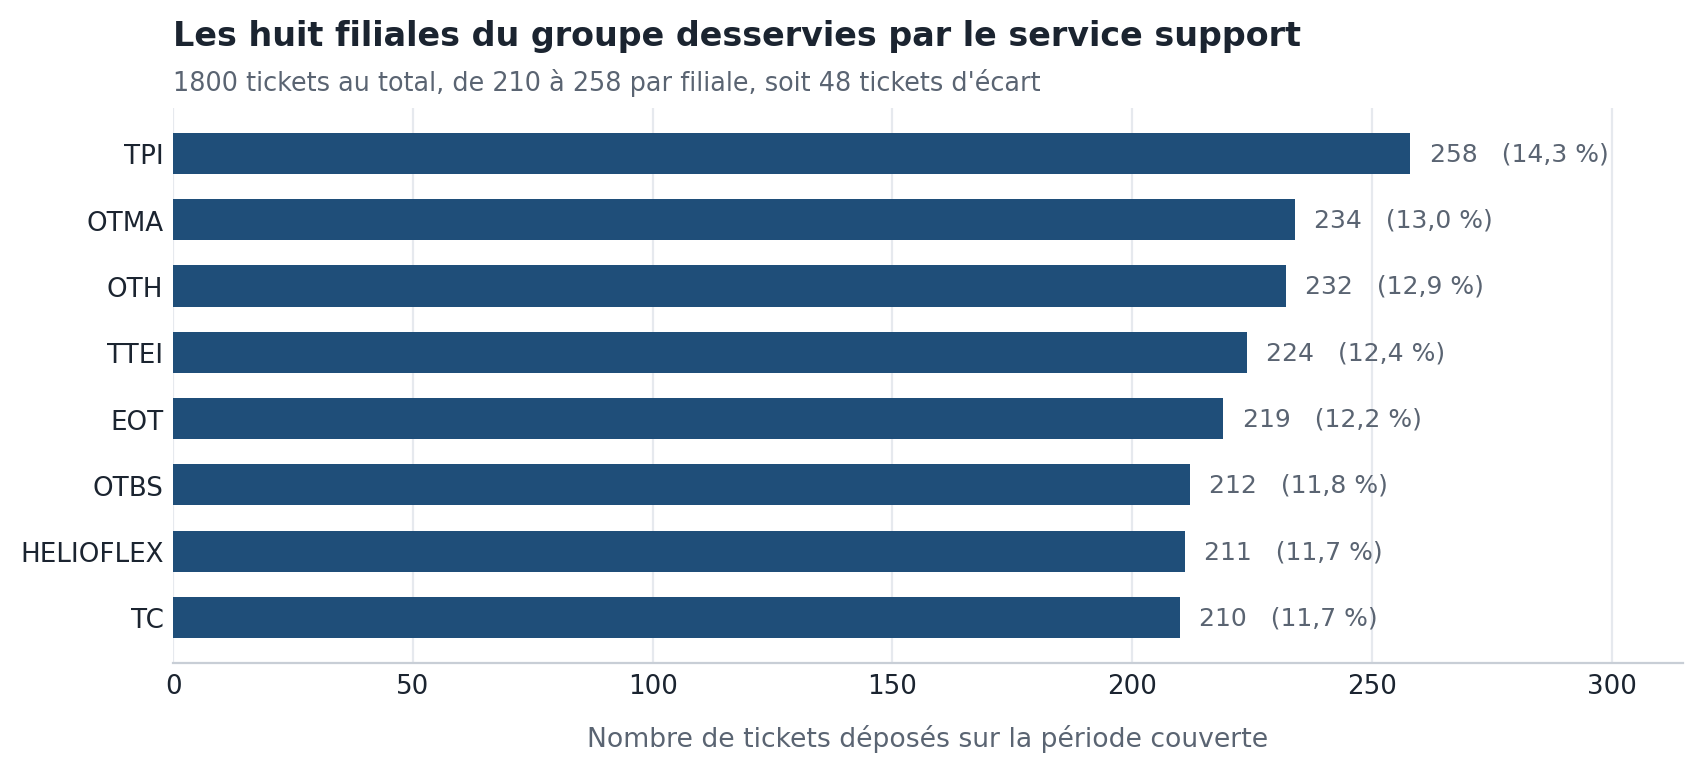
\includegraphics[width=\textwidth]{ch01_repartition_entites.png}
\caption{Répartition des tickets entre les huit filiales desservies}
\label{fig:entites1}
\end{figure}

La charge est remarquablement plate : 48 tickets séparent la filiale la plus demandeuse de la moins
demandeuse, soit un écart de 23\,\% sur des volumes compris entre 210 et 258. Aucune filiale ne
domine le service. Les libellés portés sur la figure sont les codes du fichier d'export, et \OTBS y
figure au même titre que les autres, le service assurant aussi le support de sa propre société.

Le support est donc une fonction mutualisée, servie par une équipe restreinte au profit d'une
population plus de dix-huit fois plus nombreuse. Les applications, les usages et le vocabulaire
varient d'une filiale à l'autre, ce qui élargit la diversité des formulations qu'un modèle de
classification devra absorber.

Les demandes sont classées selon un référentiel de huit catégories : Microsoft, Réseau, Applicatifs,
Infrastructure, Système, Communication, Sécurité et Backup. Leur fréquence est très inégale, le
rapport entre la plus courante et la plus rare atteignant 5,93. Ce déséquilibre constituera la
principale difficulté du travail de modélisation conduit au chapitre~4.

Deux autres classements coexistent avec celui-là dans le fichier. Une colonne de classification
range chaque ticket parmi cinq natures, la demande, le problème, l'incident, l'alerte et le
changement. Une colonne de priorité en distingue quatre, du mineur au critique. Le service dispose
donc déjà d'un vocabulaire de gestion de services, sans qu'aucun de ces trois axes ne soit exploité
autrement que par lecture humaine.

\textbf{Volumétrie observée.} Le corpus couvre quatorze mois, du 1\textsuperscript{er} janvier 2025 au 17 février 2026, pour
1\,800 tickets déposés. La figure~\ref{fig:volumetrie} en donne la répartition mensuelle.

\begin{figure}[!htbp]
\centering
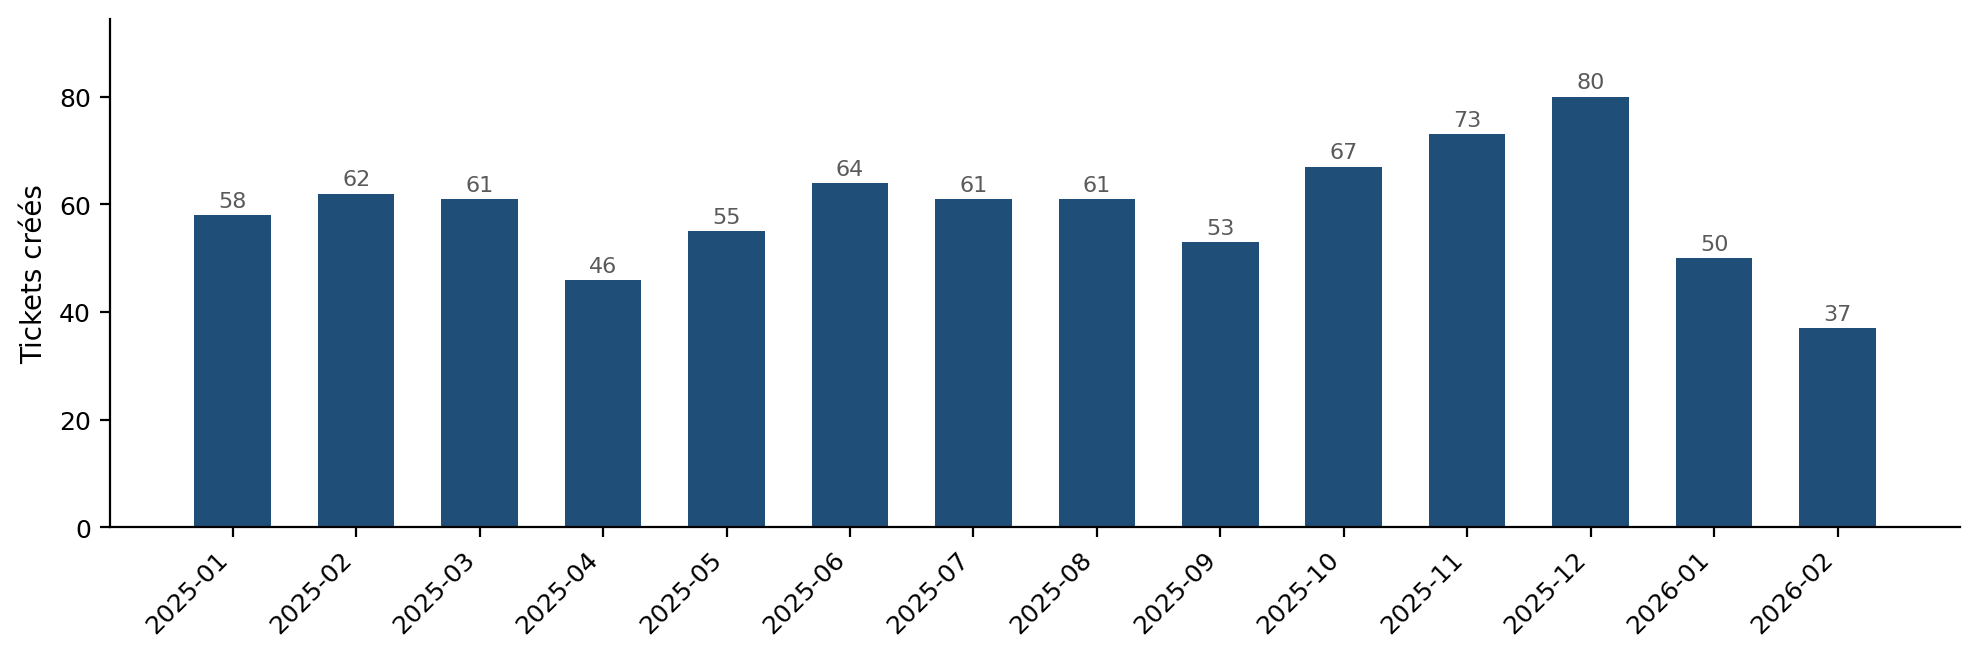
\includegraphics[width=\textwidth]{ch01_volumetrie_mensuelle.png}
\caption{Tickets déposés par mois sur la période couverte par l'export}
\label{fig:volumetrie}
\end{figure}

L'activité est remarquablement stable, autour de 129 tickets par mois, soit environ six par jour
ouvré. Aucune saisonnalité marquée n'apparaît. Le dernier mois est partiel, l'export s'arrêtant au
17 février, et la figure le signale pour éviter d'y lire une chute d'activité.

Cette stabilité a une conséquence pratique pour la suite. Un service dont la charge ne varie pas
n'a pas de pic à absorber, et le gain attendu d'une assistance automatique ne réside donc pas dans
l'écrêtage d'une surcharge. Il réside dans le temps passé, ticket après ticket, sur des gestes que
la section~\ref{sec:repetitivite} montre concentrés sur un petit nombre de cas.

\textbf{L'outil de suivi et la qualité de ses données.} L'enregistrement reposait sur une liste SharePoint. Nous ne le déduisons pas d'un entretien mais du
fichier d'export : la colonne \texttt{Chemin d'accès} porte, sur les 1\,800 lignes et sans exception,
la valeur \texttt{sites/IT-Check/Lists/HelpDesk}. Une telle liste assure la saisie et
l'historisation, sans offrir ni tri automatique ni recherche dans les résolutions passées. Surtout,
elle ne contient que ce qu'un consultant a pris le temps d'y consigner.

L'export porte dix-huit colonnes, dont six ne sont pas systématiquement renseignées : la
priorité, l'affectation, l'analyse, la résolution, l'identifiant de rattachement et la date de
résolution. Le chapitre~2 en donne les taux et les interprète, la qualité des données relevant de
l'étude du corpus plutôt que de l'état des lieux du service.


Un défaut plus discret mérite d'être signalé, car il illustre ce qu'une saisie sans contrôle
produit. La colonne des dates de création mêle deux formats, 972 lignes au format jour, mois, année
et 828 au format année, mois, jour. Une lecture naïve du fichier n'en interprète qu'un seul et perd
silencieusement 46\,\% du corpus. Le chapitre~3 revient sur les nettoyages que cet état de fait a
rendus nécessaires.

\textbf{Le cycle de vie du ticket.} Le processus n'ayant jamais été formalisé, nous l'avons déduit des données. Le champ \texttt{STATUT}
prend cinq valeurs qui décrivent un cycle de vie complet, restitué à la figure~\ref{fig:processus}.

\begin{figure}[!htbp]
\centering
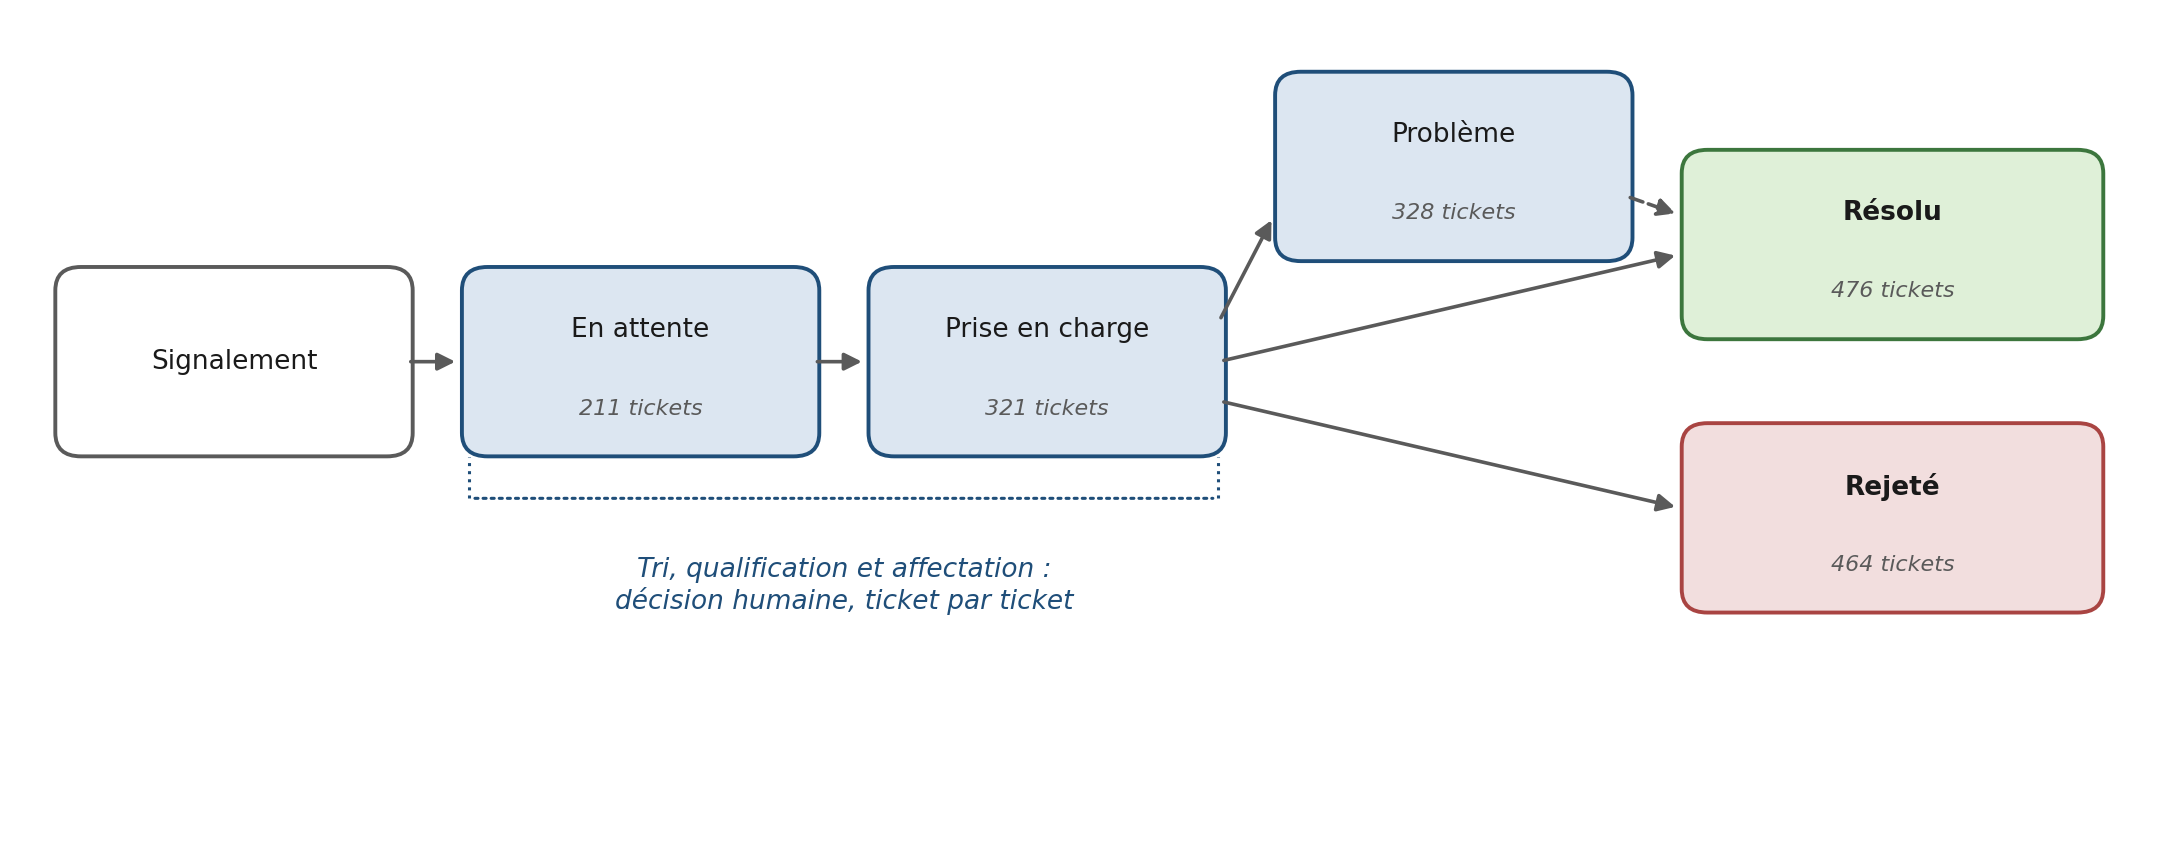
\includegraphics[width=\textwidth]{ch01_processus_existant.png}
\caption{Cycle de vie du ticket avant le projet, reconstitué à partir du champ \texttt{STATUT}}
\label{fig:processus}
\end{figure}

Le tri, la qualification et l'affectation se logent entre le dépôt et la prise en charge. Ce sont
des décisions humaines, prises ticket après ticket, et le fichier n'en garde aucune trace autre que
leur résultat. L'étape de qualification commande tout le reste, car décider de la catégorie d'un
ticket revient à décider qui va le traiter. Une catégorie mal choisie oriente la demande vers une
compétence qui n'est pas la bonne, et le temps est perdu deux fois. La classification automatique
que nous proposons répond d'abord à ce besoin d'aiguillage.

Un chiffre retient l'attention sur cette figure : 464 tickets rejetés pour 476 résolus. Près d'une
demande sur deux parvenue à son terme se solde par un refus. Ce taux renseigne moins sur la
difficulté des cas soumis au service que sur l'absence de contrôle à l'entrée. Le fichier
n'enregistre aucun motif structuré de rejet, et nous ne pouvons donc pas en décomposer les causes.

\label{sec:repetitivite}

\textbf{Répétitivité des résolutions.} Une dernière observation achève de caractériser ce travail. Sur les 1\,800 tickets du corpus, la
colonne consacrée aux gestes de résolution ne compte que 58 valeurs distinctes. Les colonnes de
titre, d'analyse et de base de connaissances en comptent exactement autant, ce qui indique qu'elles
sont solidaires : le service traite cinquante-huit situations types, répétées une trentaine de fois
chacune en moyenne.

Les descriptions libres, elles, comptent 1\,535 valeurs distinctes. L'écart entre ces deux nombres
résume le problème du service. Les utilisateurs formulent leurs demandes de mille manières, alors
que les réponses appartiennent à un répertoire restreint et stable. Retrouver la bonne réponse est
un travail de reconnaissance, non d'invention.

Le temps des consultants se concentre alors sur des tâches sans valeur ajoutée technique :
qualifier la demande pour l'orienter, retrouver un cas comparable dans l'historique, rédiger la
réponse au demandeur. Aucune n'exige l'expertise pour laquelle ils ont été recrutés.

\textbf{Limites du diagnostic.} L'honnêteté du diagnostic exige d'en marquer les bords. Plusieurs éléments qu'un état des lieux
complet comporterait nous ont manqué, faute de réponse à la demande d'informations adressée à
l'entreprise. Nous les énonçons ici plutôt que de les combler par des suppositions.

Nous ne disposons ni d'organigramme du service, ni de description de ses niveaux d'intervention, ni
d'engagement de niveau de service formalisé. Le fichier ne dit rien du canal par lequel chaque
demande est arrivée, de sorte que la part des sollicitations passées par téléphone ou de vive voix
reste inconnue. Le temps moyen de traitement d'un ticket n'a pas été confirmé, et nous ne le citons
donc nulle part dans ce mémoire. Enfin, le motif des rejets n'est pas structuré dans les données.

Ces manques limitent la portée du diagnostic sur un point précis : nous ne pouvons pas chiffrer le
gain de temps attendu de la plateforme. Ils ne l'affaiblissent pas sur ce que les données montrent
directement, à savoir la répétitivité du travail, le déséquilibre des catégories, le taux de rejet
et l'absence de mémoire interrogeable. Ce risque est suivi au registre du projet.

\subsection{Limites de l'existant et solutions du marché}

Le tableau~\ref{tab:limites} met les limites constatées en regard du besoin qu'elles engendrent.

\begin{table}[!htbp]
\centering
\styletableau
\caption{Limites de l'existant et besoins associés}
\label{tab:limites}
\begin{tabular}{|Bp{6.6cm}|Lp{7.4cm}|}
\hline
\rowcolor{enteteTab}
\textbf{Limite constatée} & \textbf{Besoin qui en découle} \\
\hline
Aucun point d'entrée ne garantit qu'une intervention laisse une trace &
Offrir un point d'entrée unique et structuré \\
\hline
Le demandeur n'a aucune visibilité sur l'avancement de sa demande &
Donner au demandeur un suivi autonome de ses tickets \\
\hline
L'orientation du ticket repose sur un jugement manuel, refait à chaque demande &
Proposer automatiquement une catégorie, assortie d'un indicateur de fiabilité \\
\hline
L'historique des résolutions n'est pas interrogeable &
Retrouver les cas comparables et leurs sources à partir d'une description libre \\
\hline
La connaissance produite reste attachée aux personnes &
Capitaliser automatiquement chaque résolution validée \\
\hline
La saisie n'est soumise à aucun contrôle, d'où des champs vides et des formats mêlés &
Contrôler la saisie à la source plutôt qu'après coup \\
\hline
\end{tabular}
\end{table}

Ces limites partagent une même origine : le dispositif en place enregistre une partie de
l'information, après coup, sans jamais l'exploiter.

\textbf{Les solutions du marché.} Trois familles d'outils auraient pu répondre au besoin, et aucune ne le fait entièrement dans notre
contexte.

Les plateformes en mode service, telles Zendesk ou Freshdesk, supposent l'hébergement des données
chez l'éditeur, ce que la contrainte de confidentialité exclut d'emblée. Les solutions libres
hébergeables en interne, GLPI au premier rang, assurent la gestion du cycle de vie du ticket sans
proposer nativement de classification apprise sur l'historique du service. Les suites complètes de
gestion des services informatiques, du type ServiceNow, sont dimensionnées pour des organisations
d'une tout autre échelle que celle d'une équipe de onze personnes.

Le tableau~\ref{tab:marche1} confronte ces trois familles aux trois exigences que le contexte
impose. Aucune colonne n'est pleine, et c'est ce constat qui fonde la problématique du projet.

\begin{table}[!htbp]
\centering
\singlespacing
\styletableau
\renewcommand{\arraystretch}{1.25}
\caption{Les trois familles d'outils du marché face aux exigences du contexte}
\label{tab:marche1}
\begin{tabular}{|Lp{4.0cm}|Cp{3.1cm}|Cp{3.1cm}|Cp{3.3cm}|}
\hline
\rowcolor{enteteTab}
\textbf{Exigence du contexte} &
\textbf{Plateformes en mode service}\newline \small\textit{Zendesk, Freshdesk} &
\textbf{Solutions libres hébergeables}\newline \small\textit{GLPI} &
\textbf{Suites complètes de gestion}\newline \small\textit{ServiceNow} \\
\hline
Les données ne quittent pas l'infrastructure de l'entreprise &
\cellcolor{refus}\textbf{Non}\newline \small hébergement chez l'éditeur &
\cellcolor{tenu}\textbf{Oui} &
\cellcolor{tenu}\textbf{Oui} \\
\hline
Classification apprise sur l'historique propre au service &
\cellcolor{tenu}\textbf{Oui} &
\cellcolor{refus}\textbf{Non}\newline \small pas de classification native &
\cellcolor{tenu}\textbf{Oui} \\
\hline
Dimensionnement adapté à une équipe de onze personnes &
\cellcolor{tenu}\textbf{Oui} &
\cellcolor{tenu}\textbf{Oui} &
\cellcolor{refus}\textbf{Non}\newline \small échelle bien supérieure \\
\hline
\end{tabular}
\end{table}

Aucune famille ne réunit simultanément le traitement du français métier tel que ce service l'écrit,
l'exécution sur l'infrastructure de l'entreprise et l'exploitation de l'historique propre au
service.

\subsection{Problématique}

\begin{center}
\begin{minipage}{0.92\textwidth}
\itshape
Comment classer automatiquement et de manière fiable des tickets informatiques francophones, courts,
déséquilibrés et bruités, et proposer une assistance à la résolution pertinente et vérifiable, tout
en conservant un contrôle humain sur la décision finale ?
\end{minipage}
\end{center}

\vspace{2mm}

Cette problématique se décline en questions de recherche qui structurent les travaux des
chapitres~4 et~5. Un modèle de langue francophone spécialisé améliore-t-il significativement la
classification par rapport à une approche lexicale classique, en particulier sur les catégories
minoritaires ? Une recherche sémantique fondée sur des représentations vectorielles denses
surpasse-t-elle une recherche lexicale ? Comment calibrer la confiance du modèle pour définir un
seuil au-delà duquel sa proposition peut être tenue pour suffisamment sûre ?

\section{Solution proposée et périmètre du travail}

Nous proposons une plateforme, nommée HelpDesk AI, dont la figure~\ref{fig:solution} donne la vue
fonctionnelle.

\begin{figure}[!htbp]
\centering
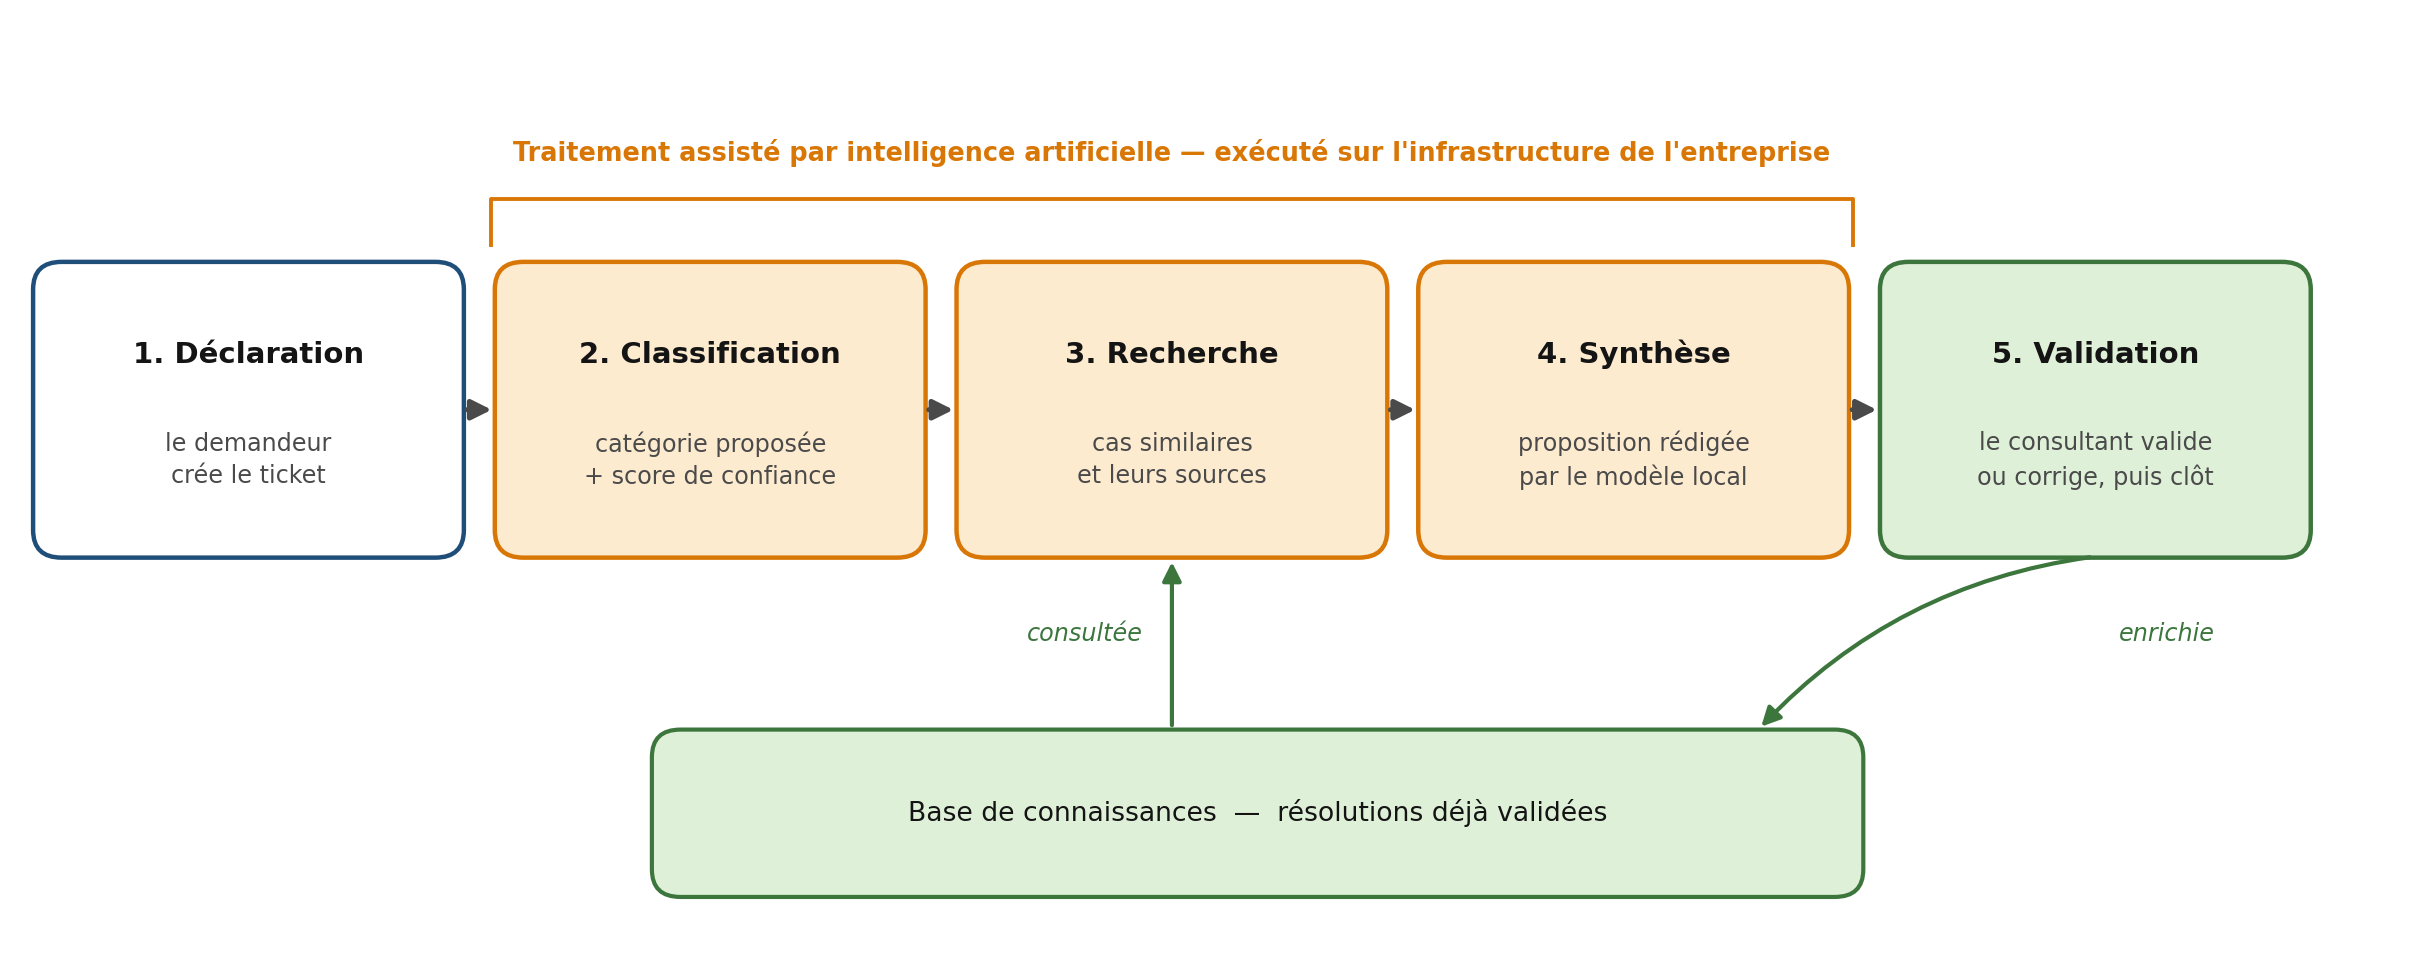
\includegraphics[width=\textwidth]{ch01_vue_solution.png}
\caption{Vue fonctionnelle de la solution proposée}
\label{fig:solution}
\end{figure}

Elle est d'abord le point d'entrée qui faisait défaut : toute demande y est déclarée par le
demandeur lui-même dans un formulaire structuré, de sorte qu'aucune intervention n'échappe plus à
l'historique. Viennent ensuite les briques d'assistance. Le classifieur automatique attribue une
catégorie à chaque ticket entrant et retourne un score de confiance, qui appuie la décision
d'orientation. Le moteur de recherche par similarité interroge l'historique des résolutions et
remonte les cas les plus proches avec leurs sources, de sorte que chaque suggestion reste
vérifiable. Le modèle de langage exécuté localement synthétise enfin ces cas en une proposition
rédigée, sans qu'aucune donnée ne quitte l'infrastructure de l'entreprise.

Le principe directeur est le maintien de la décision humaine : le système propose, le consultant
tranche. Aucune décision n'est appliquée sans validation, et chaque validation alimente en retour la
base de connaissances. L'application distingue en conséquence deux parcours, un portail où le
demandeur crée et suit ses tickets, et une console d'administration où le consultant examine les
propositions, les corrige si nécessaire et clôt les demandes.

\textbf{Périmètre du travail.} Reste à délimiter le périmètre, ce que fait le tableau~\ref{tab:perimetre}. Poser cette frontière
dès le cadrage protège l'évaluation contre le reproche de ne pas avoir traité ce qui n'a jamais été
promis.

\begin{table}[!htbp]
\centering
\styletableau
\caption{Périmètre retenu et hors-périmètre}
\label{tab:perimetre}
\begin{tabular}{|Bp{6.9cm}|Lp{7.1cm}|}
\hline
\rowcolor{enteteTab}
\textbf{Inclus dans le périmètre} & \textbf{Exclu du périmètre} \\
\hline
Chaîne de données documentée, versionnée et reproductible &
Mise en production sur l'infrastructure du groupe \\
\hline
Classifieur automatique évalué sur protocole explicite &
Intégration au système d'information existant \\
\hline
Moteur d'assistance à la résolution et modèle de langage local &
Reprise et migration des tickets historiques \\
\hline
Application web complète, portail demandeur et console d'administration &
Notifications automatiques sur changement de statut \\
\hline
Conteneurisation et chaîne de traitement reproductible &
Supervision en exploitation et reprise sur incident \\
\hline
\end{tabular}
\end{table}

Le livrable attendu est une plateforme démontrable et documentée, accompagnée d'une évaluation
honnête de ce qu'elle apporte et de ses limites. Sa mise en exploitation reste hors sujet.

\textbf{Les contraintes qui ont pesé.} Quatre contraintes ont pesé sur le travail du cadrage jusqu'à la
soutenance. Le
tableau~\ref{tab:contraintes1} les réunit avec ce que chacune a écarté.

\begin{table}[!htbp]
\centering
\singlespacing
\styletableau
\renewcommand{\arraystretch}{1.15}
\caption{Contraintes du projet, leur origine et ce qu'elles ont écarté}
\label{tab:contraintes1}
\begin{tabular}{|Bp{2.9cm}|Lp{5.4cm}|Lp{4.8cm}|}
\hline
\rowcolor{enteteTab}
\textbf{Contrainte} & \textbf{Origine} & \textbf{Ce qu'elle a écarté} \\
\hline
Confidentialité des tickets &
Règles de sécurité de l'entreprise, énoncées à la session d'intégration et reprises en ENF-04 &
Les services d'inférence hébergés. Le modèle de langage s'exécute sur place, ce qui pèse sur le
temps de réponse \\
\hline
Un corpus étroit &
L'historique que le service a pu fournir : 1\,800 lignes, 58 types de demandes, 8 catégories dont
deux réunissent moins de cinq pour cent des tickets &
L'entraînement d'un modèle depuis zéro. Le travail porte sur l'adaptation d'un modèle déjà
pré-entraîné \\
\hline
Un matériel modeste &
Le processeur graphique mis à disposition dispose de 2\,Go de mémoire vidéo &
L'ajustement complet d'un transformer. L'adaptation à faible rang répond à cette limite \\
\hline
La décision reste humaine &
Principe posé au cadrage avec le service support &
La clôture prononcée par le système. Toute demande passe par une file d'approbation \\
\hline
\end{tabular}
\end{table}

Ces contraintes ne sont pas des obstacles rencontrés en chemin. Elles étaient connues au cadrage,
elles commandent les choix techniques des chapitres~4 et~5, et le chapitre~6 chiffre ce qu'elles ont
coûté.

\label{sec:positionnement2}

\textbf{Ce que le travail apporte en propre.} Les techniques mobilisées sont d'usage courant. Ce
qui distingue ce travail tient aux conditions dans lesquelles elles sont mises en œuvre et à ce que
nous avons choisi de mesurer : l'apport de règles métier ajoutées à un modèle statistique, mesuré au
lieu d'être supposé, et des scores obtenus sous un découpage qui regroupe les tickets par type avant
le tirage, précaution qui empêche un même type de demande de figurer à la fois dans l'apprentissage
et dans l'évaluation. Les chapitres~4 et~6 rapportent ces mesures. Elles valent dans les limites de
leur cadre : un seul service, une seule entreprise, un corpus francophone dont la faible diversité
interdit de présumer que les résultats se transporteraient ailleurs.

\section{Analyse et spécification des besoins}

\label{sec:besoins1}

Le besoin décrit plus haut se traduit ici en exigences vérifiables, chacune portant un
identifiant auquel les chapitres suivants se réfèrent.

\subsection{Objectifs du projet}
\label{sec:objectifs1}

Sept objectifs résument ce que la plateforme doit accomplir. Doter le service d'un point
d'entrée unique où aucune demande n'échappe à l'historique. Proposer une catégorie à chaque
demande entrante, sans laisser passer celles qui relèvent de la sécurité. Remonter des
résolutions passées comparables avec leurs sources, et les présenter assez vite pour que l'outil
soit préféré à la lecture directe du ticket. Laisser la décision à l'administrateur, aucune
clôture n'étant prononcée par le système. Rendre enfin la chaîne de traitement des données et
des modèles rejouable à l'identique.

Chacun se traduit dans les pages qui suivent en exigences numérotées, dont le critère
d'acceptation permet au chapitre~6 de conclure sans avoir à juger du résultat.

\subsection{Acteurs du système}

La plateforme distingue deux profils, récapitulés au tableau~\ref{tab:acteurs}. Cette distinction se
traduit directement dans le contrôle d'accès RBAC de l'application, qui ne connaît que deux rôles.

\begin{table}[!htbp]
\centering
\styletableau
\caption{Acteurs du système et responsabilités associées}
\label{tab:acteurs}
\begin{tabular}{|Bp{3.4cm}|Cp{2.2cm}|Lp{8.2cm}|}
\hline
\rowcolor{enteteTab}
\textbf{Acteur} & \textbf{Rôle} & \textbf{Responsabilités} \\
\hline
Demandeur & \texttt{client} & Créer une demande, suivre son avancement, consulter la réponse
apportée \\
\hline
Administrateur & \texttt{admin} & Traiter les tickets : consulter la qualification proposée et les
cas comparables avec leurs sources, valider ou corriger, répondre au demandeur. Superviser
l'activité : volumes, catégories, délais, gestion des comptes \\
\hline
\end{tabular}
\end{table}

Les administrateurs sont les consultants du service support eux-mêmes ; le terme désigne leur rôle
dans l'application, non une fonction distincte dans l'organisation. Ce regroupement du traitement et
de la supervision s'écarte des référentiels de gestion de services informatiques, qui séparent
l'agent du responsable. Cette séparation n'aurait ici aucun objet : le service compte onze
consultants qui traitent les demandes et suivent collectivement l'activité, sans échelon
intermédiaire.

Le demandeur n'a délibérément aucune visibilité sur les mécanismes de classification : ni la
catégorie prédite ni l'index de confiance ne lui sont présentés. Exposer une prédiction incertaine à
un utilisateur non spécialiste reviendrait à lui faire porter un arbitrage qui ne lui revient pas.

\subsection{Besoins fonctionnels}

Chaque exigence porte un critère d'acceptation vérifiable et un niveau de priorité : \textbf{élevée}
lorsqu'elle conditionne la livraison, \textbf{moyenne} lorsque son report resterait acceptable,
\textbf{faible} pour un apport de confort. Le tableau~\ref{tab:ef} les regroupe par niveau ; la
colonne \emph{Domaine} rappelle à quelle partie du parcours du ticket chacune se rattache.

\begin{table}[!htbp]
\centering
\styletableau
\caption{Exigences fonctionnelles et critères d'acceptation}
\label{tab:ef}
% Meme interligne resserre que le tableau des exigences non fonctionnelles :
% les deux tableaux de specification gardent ainsi la meme densite.
\renewcommand{\arraystretch}{1.25}
\begin{tabular}{|Cp{1.3cm}|Lp{4.2cm}|Lp{5.1cm}|Lp{2.5cm}|}
\hline
\rowcolor{enteteTab}
\textbf{Réf.} & \textbf{Exigence} & \textbf{Critère d'acceptation} & \textbf{Domaine} \\
\hline
\multicolumn{4}{|l|}{\cellcolor{enteteTab}\textbf{Priorité élevée} : conditionne la livraison} \\
\hline
EF-01 & Authentification et gestion des rôles & Accès restreint selon le rôle, jeton vérifié à chaque appel & Cycle de vie \\
\hline
EF-02 & Création d'un ticket par le demandeur & Ticket persisté, statut initial renseigné & Cycle de vie \\
\hline
EF-03 & Journal d'audit des modifications & Chaque changement tracé avec son auteur et sa date & Cycle de vie \\
\hline
EF-04 & Suivi du ticket par le demandeur & Statut et réponse consultables & Cycle de vie \\
\hline
EF-05 & Classification automatique en catégorie & Catégorie et index de confiance retournés & Traitement \\
\hline
EF-06 & Recherche de cas comparables & Trois résolutions proposées avec leurs sources & Traitement \\
\hline
EF-07 & Orientation selon l'index de confiance & Cas peu assurés dirigés vers une revue humaine & Traitement \\
\hline
EF-08 & Validation ou correction par l'administrateur & Catégorie finale et solution enregistrées & Qualité \\
\hline
\multicolumn{4}{|l|}{\cellcolor{enteteTab}\textbf{Priorité moyenne} : le report resterait acceptable} \\
\hline
EF-09 & Synthèse rédigée à l'attention du consultant & Réponse formulée, sources citées, garde-fous actifs & Traitement \\
\hline
EF-10 & Recueil du retour du demandeur & Avis persisté et exploitable & Qualité \\
\hline
EF-11 & Résumé automatique du ticket & Résumé affiché à l'administrateur & Qualité \\
\hline
EF-12 & Suggestion de priorité & Niveau proposé à la prise en charge & Qualité \\
\hline
\multicolumn{4}{|l|}{\cellcolor{enteteTab}\textbf{Priorité faible} : apport de confort} \\
\hline
EF-13 & Analyse de tonalité du message & Indicateur d'urgence affiché & Qualité \\
\hline
EF-14 & Tableau de bord d'activité & Volumes, catégories et délais consultables & Qualité \\
\hline
\end{tabular}
\end{table}

% Le commentaire qui suit porte sur le tableau : la barriere empeche le flottant
% de deriver apres lui, ce qui ferait lire l'explication avant la piece expliquee.

Le classement en trois niveaux suit les dépendances du parcours d'un ticket. Les huit exigences de
priorité élevée forment la chaîne minimale sans laquelle une demande ne peut ni exister, ni être
qualifiée, ni être tranchée : la déposer (EF-02), la qualifier (EF-05, EF-06, EF-07), décider de son
sort (EF-08), la suivre (EF-04) et savoir qui est intervenu (EF-01, EF-03). En retirer une seule
interrompt le parcours décrit plus haut, et la solution cesse alors de répondre au problème qui
l'a motivée.

Les exigences de priorité moyenne allègent le travail du consultant sans conditionner ce parcours.
Un ticket se traite sans synthèse rédigée ni résumé automatique : le consultant lit la description
lui-même, comme il le faisait avant l'outil. Celles de priorité faible n'interviennent pas dans le
traitement d'une demande ; elles servent à observer l'activité une fois celle-ci traitée.

Une exigence appelle une réserve, posée ici plutôt que laissée à la découverte du lecteur :
l'exigence EF-09 s'appuie sur des gabarits de texte et non sur une génération libre par le modèle
de langage.

\subsection{Besoins non fonctionnels}

Les exigences non fonctionnelles fixent les seuils que la solution devra tenir, et ce sont eux que le chapitre~6 confrontera aux mesures.

% Placement [H] : le tableau doit suivre immediatement le titre de la sous-section.
% En [!htbp] il flottait vers la page suivante et laissait une demi-page blanche.
\begin{table}[H]
\centering
\styletableau
\caption{Exigences non fonctionnelles}
\label{tab:enf}
% Interligne resserre et colonne d'exigence elargie : neuf lignes tiennent ainsi
% sous le titre de la sous-section, au lieu d'imposer une page a elles seules.
\renewcommand{\arraystretch}{1.05}
\begin{tabular}{|Cp{1.4cm}|Bp{3.2cm}|Lp{9.4cm}|}
\hline
\rowcolor{enteteTab}
\textbf{Réf.} & \textbf{Catégorie} & \textbf{Exigence} \\
\hline
ENF-01 & Performance & Prédiction et recherche servies sous 300\,ms au quatre-vingt-quinzième centile \\
\hline
ENF-02 & Qualité de l'IA & F1-macro du classifieur d'au moins 0,85, mesuré selon un protocole arrêté
avant l'expérimentation \\
\hline
ENF-03 & Qualité de l'IA & Rappel d'au moins 0,70 sur la catégorie \emph{Sécurité} \\
\hline
ENF-04 & Confidentialité & (a) Aucune donnée de ticket transmise à un service externe ;
(b) traitement des données personnelles conforme à la réglementation \\
\hline
ENF-05 & Sécurité & Authentification par jeton, contrôle d'accès RBAC, secrets non exposés \\
\hline
ENF-06 & Fiabilité & Fonctionnement dégradé mais opérationnel en cas d'indisponibilité du modèle de
langage \\
\hline
ENF-07 & Maintenabilité & Code structuré en couches et couvert par des tests automatisés \\
\hline
ENF-08 & Reproductibilité & Chaîne de traitement des données et des modèles réexécutable à l'identique \\
\hline
ENF-09 & Portabilité & Déploiement conteneurisé sur une infrastructure standard \\
\hline
\end{tabular}
\end{table}

Le tableau~\ref{tab:enf} référence les exigences non fonctionnelles sur le même principe que les
exigences fonctionnelles, de sorte que les chapitres suivants puissent s'y référer sans ambiguïté.

Ces neuf exigences ne proviennent pas d'un référentiel appliqué par principe. Chacune répond à une
propriété que le service attendait ou à une contrainte qui s'imposait au projet. Le temps de réponse
(ENF-01) tient à ce qu'un outil plus lent que la lecture directe d'un ticket ne serait pas adopté.
Le rappel sur la catégorie \emph{Sécurité} (ENF-03) tient à ce qu'elle compte parmi les plus rares du
référentiel et que l'erreur y coûte le plus cher. Le fonctionnement dégradé (ENF-06) tient à ce que
le modèle de langage s'exécute sur une machine de l'entreprise, donc peut cesser de répondre.

L'exigence ENF-04 occupe une place à part. Les autres se négocient, une latence pouvant être améliorée ou
une couverture de tests complétée. Celle-ci traduit une règle interne de l'entreprise et une
obligation réglementaire sur les données personnelles. Elle a été traitée comme un axiome de
conception, et c'est elle qui a imposé l'exécution locale du modèle de langage.

Ses deux volets n'ont cependant pas connu le même sort, et nous les distinguons dès leur énoncé
pour que le bilan du chapitre~6 puisse les juger séparément. Le volet (a), l'absence de service
externe, relève de l'architecture et se vérifie dans le code livré. Le volet (b), le traitement des
données personnelles, se partage entre un traitement technique et une décision d'organisation :
pseudonymisation du corpus d'un côté, durée de conservation et information des personnes de
l'autre. Le premier a été mis en œuvre et vérifié ; les deux autres dépassent le cadre du stage, et
présenter le volet comme entièrement satisfait serait inexact. La section~\ref{sec:rgpd} en
détaille la portée exacte, et le bilan du chapitre~6 le déclare partiellement tenu.

\textbf{Traçabilité des exigences.} Le tableau~\ref{tab:tracabilite} rattache chaque domaine d'exigences au chapitre qui en rend compte.
La conclusion générale revient sur celles que la solution livrée ne tient pas.

\begin{table}[!htbp]
\centering
\styletableau
\caption{Traçabilité des exigences vers les chapitres de traitement}
\label{tab:tracabilite}
\begin{tabular}{|Bp{6.4cm}|Cp{2.2cm}|Lp{4.6cm}|}
\hline
\rowcolor{enteteTab}
\textbf{Domaine d'exigences} & \textbf{Chapitre} & \textbf{Nature du traitement} \\
\hline
Gouvernance et qualité des données & 3 & Constitution du corpus, séparation anti-fuite,
versionnement \\
\hline
Classification automatique, qualité de l'IA & 4 & Comparaison des approches, évaluation \\
\hline
Assistance à la résolution, confidentialité & 5 & Moteur de similarité, modèle de langage local \\
\hline
Cycle de vie, accès, boucle de qualité & 7 & Application web, workflow, validation humaine \\
\hline
Sécurité, fiabilité, reproductibilité, portabilité & 3 et 7 & Traitement transverse au fil des
chapitres, bilan de conformité au chapitre~6 \\
\hline
\end{tabular}
\end{table}

\section{Méthodologie de travail}

Le projet mêle du développement logiciel, dont le résultat se planifie, et de
l'expérimentation, dont le résultat ne se planifie pas. Le choix d'une démarche devait
tenir compte des deux.

\subsection{Comparaison des démarches envisagées}

Trois démarches de conduite ont été examinées avant de trancher, chacune portant une
conception différente de ce qui peut être planifié à l'avance.

\begin{table}[H]
\centering
% Place avec [H] pour rester sous le titre. Le paquet float court-circuite le
% reglage d'interligne que setspace applique aux flottants : on le retablit ici.
\singlespacing
\styletableau
\caption{Comparaison des démarches de conduite de projet}
\label{tab:methodo}
\begin{tabular}{|Bp{3.1cm}|Lp{3.5cm}|Lp{3.5cm}|Lp{3.5cm}|}
\hline
\rowcolor{enteteTab}
\textbf{Critère} & \textbf{Cycle en V} & \textbf{Scrum} & \textbf{CRISP-DM} \\
\hline
Nature du besoin & Figé en amont & Évolutif & Exploratoire \\
\hline
Progression & Séquentielle, une seule passe & Itérative, incréments livrables & Itérative, retours
entre phases \\
\hline
Gestion de l'incertitude & Faible & Bonne sur le produit & Bonne sur la donnée \\
\hline
Livrable intermédiaire & Documents de spécification & Incrément fonctionnel & Modèle évalué \\
\hline
Limite dans notre contexte & Les résultats d'un modèle ne se planifient pas & Ne couvre pas le cycle
de vie de la donnée & Ne décrit pas le développement applicatif, rattaché ici au déploiement \\
\hline
\end{tabular}
\end{table}

Le tableau~\ref{tab:methodo} compare sur cinq critères les trois démarches examinées.
Le projet relève de deux natures de travail que les démarches classiques traitent rarement ensemble.
Il comporte un volet de développement logiciel, où le besoin est identifiable et le résultat
prévisible, et un volet de science des données, où le résultat d'une expérimentation ne peut par
définition être garanti à l'avance. Nous avons examiné trois démarches candidates.

Le cycle en V suppose un besoin stabilisé et un résultat prévisible ; il aurait conduit à figer des
objectifs de performance avant toute expérimentation, ce qui n'a pas de sens en apprentissage
automatique. Scrum apporte l'itération et la livraison incrémentale, en restant centré sur le
produit logiciel et en laissant de côté la préparation et l'évaluation des données. CRISP-DM
\cite{wirth2000} structure précisément le cycle de vie de la donnée, de la compréhension du métier
jusqu'au déploiement en passant par la préparation, la modélisation et l'évaluation ; il ignore en
revanche le développement applicatif qui doit rendre le modèle utilisable.

\subsection{Démarche retenue : CRISP-DM}

CRISP-DM est la méthodologie officielle de ce projet. C'est le seul des trois cadres examinés qui
traite la préparation et l'évaluation des données comme des étapes à part entière, alors qu'elles
concentrent l'essentiel de la difficulté ici. La figure~\ref{fig:crispdm} en donne la représentation
usuelle.

% Schema fourni par l'auteur (images/crisp.jpg). Il mesure 552x510 px, ce qui donne
% environ 145 dpi a cette largeur : lisible a l'ecran, un peu doux a l'impression.
% Un export du meme schema en 1500 px de large reglerait le point sans rien changer ici.
\begin{figure}[H]
\centering
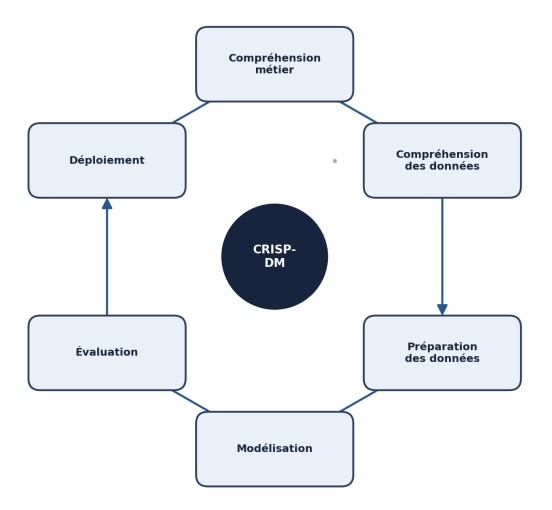
\includegraphics[width=0.62\textwidth]{ch01_crispdm.jpg}
\caption{Les six phases de la démarche CRISP-DM}
\label{fig:crispdm}
\end{figure}

Le schéma se lit comme un cycle fermé : la compréhension du métier l'ouvre, le déploiement y ramène.
C'est ce bouclage qui a joué ici. L'analyse du corpus, au chapitre~2, a fait apparaître une
contrainte que l'entretien initial n'avait pas révélée, et le chapitre~6 rapporte des résultats qui
contredisent l'hypothèse de départ. Chaque retour de ce genre a ouvert une itération nouvelle, où la
question de départ était reposée avant que le travail technique ne reprenne.

Le développement logiciel ne constitue pas une phase supplémentaire. Il se répartit entre la phase
de déploiement et d'intégration, qui dans le standard comprend la production du mécanisme de
livraison, et les itérations successives du projet. L'application du chapitre~7 est ce qui rend les
modèles utilisables, la conteneurisation du chapitre~7 ce qui les rend installables ailleurs.

La figure~\ref{fig:phases1} place les six phases en regard des sept chapitres.

\begin{figure}[H]
\centering
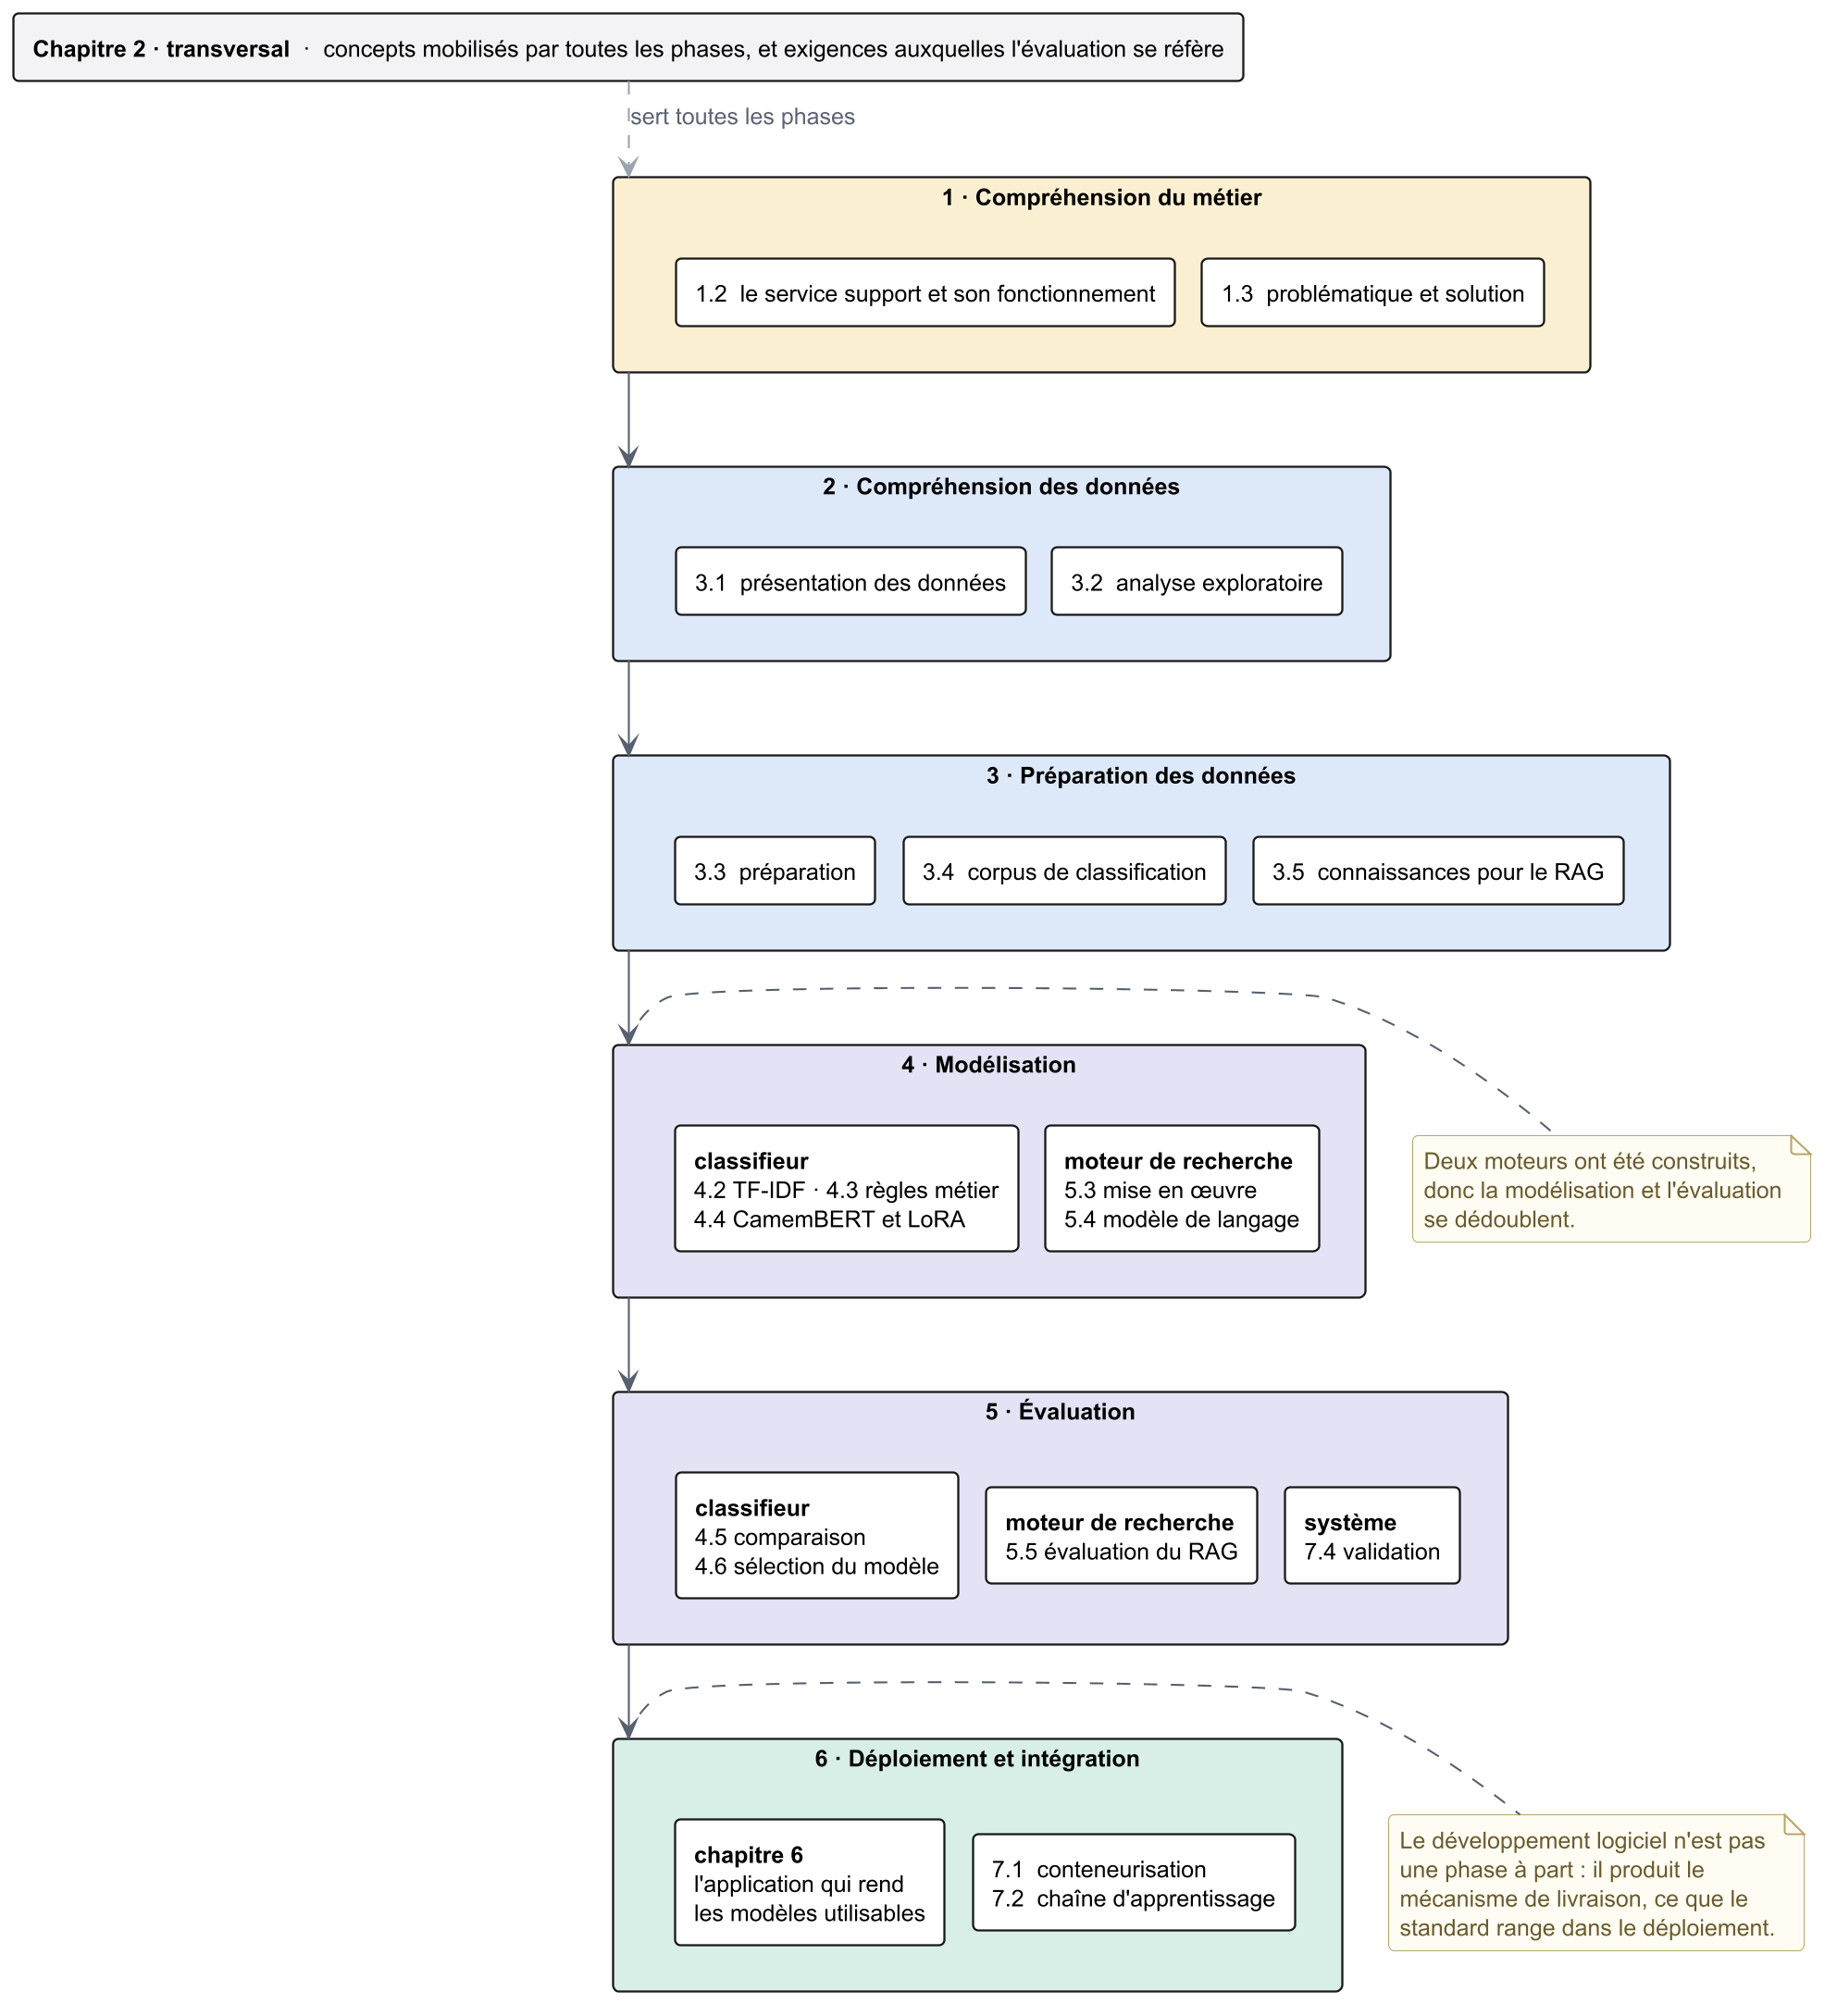
\includegraphics[width=0.98\textwidth]{ch01_crispdm_chapitres.png}
\caption{Les six phases de CRISP-DM en regard des sept chapitres du mémoire}
\label{fig:phases1}
\end{figure}

Deux traits de ce découpage méritent d'être énoncés. La modélisation et l'évaluation se dédoublent,
parce que le travail a produit deux moteurs et non un, chacun avec sa propre campagne de mesure. Et
tout n'est pas rattaché à une phase unique : les concepts théoriques sont exposés dans le chapitre qui les mobilise plutôt que rassemblés à part, et deux sections le sont également, la gouvernance des
données en 3.6 et la chaîne d'apprentissage automatisé en 7.2.

Une règle a été tenue d'un bout à l'autre, et elle engage la validité des résultats : le protocole
d'évaluation de chaque modèle a été arrêté avant son entraînement. Définir la métrique avant
l'expérimentation ferme la porte au biais qui consiste à retenir a posteriori l'indicateur le plus
flatteur. Le chapitre~6 en donne l'illustration, les résultats y étant rapportés tels qu'ils sont
sortis, y compris lorsqu'ils contredisent l'hypothèse initiale.

% Aucun flottant du corps ne doit franchir la conclusion.
\FloatBarrier

\section*{Conclusion}
\addcontentsline{toc}{section}{Conclusion}

Ce chapitre a posé le terrain du projet. Le support informatique d'\OTBS est une fonction
mutualisée : onze consultants traitent les demandes de huit filiales du groupe, pour deux cent deux
demandeurs. Les interventions sont consignées dans une liste SharePoint qui ne trie rien
automatiquement et que personne ne peut interroger.

Trois familles d'outils du marché ont été examinées. Aucune ne réunit à la fois le traitement du
français tel que ce service l'écrit, l'exécution sur l'infrastructure de l'entreprise et
l'exploitation de l'historique propre au service. Nous avons donc conçu une plateforme spécifique,
articulée autour d'un point d'entrée unique, d'un classifieur, d'un moteur de recherche par
similarité et d'un modèle de langage exécuté localement, chaque décision restant soumise à la
validation d'un consultant.

Le besoin est désormais traduit en exigences numérotées, auxquelles le chapitre~6 confrontera les
mesures. La conduite du travail suit CRISP-DM, dont les six phases commandent le découpage des
chapitres qui suivent. Le prochain ouvre la deuxième phase : comprendre les données avant de
prétendre en tirer quoi que ce soit.

        \clearpage

        \addtocontents{toc}{\protect\phasecrisp{Phase 2 --- Compréhension des données}}
\chapter{Exploration et compréhension des données}

\section*{Introduction}
\addcontentsline{toc}{section}{Introduction}

Le chapitre précédent a posé le problème et fixé les exigences. Celui-ci ouvre la deuxième phase de
la démarche, la compréhension des données. Un modèle ne vaut que ce que valent les données dont il
apprend, et l'exploration conduite ici décide de ce qui sera possible ensuite.

Nous décrivons d'abord la provenance du corpus, son schéma et la variable à prédire. Nous mesurons
ensuite sa qualité, sa distribution et sa redondance. L'analyse met au jour deux caractéristiques
qui pèsent sur toute la suite : une distribution très inégale entre catégories et une forte
redondance des situations décrites.

Aucune transformation n'est appliquée dans ce chapitre. Il observe, il mesure, et il énonce les
risques que ces mesures font peser sur la modélisation.

\section{Présentation des données}

Le corpus provient d'un export unique, dont nous décrivons la provenance, le schéma et la variable
à prédire avant toute analyse.

\subsection{Provenance et mode de collecte}

\label{sec:provenance}

Le jeu de données nous a été fourni par l'entreprise. Il rassemble les demandes traitées par le
service support dans le cadre de son activité courante : 1\,800 tickets créés entre le
1\textsuperscript{er} janvier 2025 et le 17 février 2026, soit quatorze mois d'activité et une
moyenne de 129 tickets par mois. Ils émanent de 202 demandeurs distincts répartis sur les huit
filiales du groupe, et sont assignés à onze intervenants, ce qui recoupe l'effectif du service
décrit au chapitre~1.

La saisie n'était soumise à aucun contrôle, ce dont le chapitre~1 donne l'illustration la plus
nette avec les deux formats de date qui coexistent dans un même champ. Les nettoyages que cet état
impose relèvent du chapitre~3 ; l'analyse qui suit porte sur le fichier tel qu'il a été reçu.

\subsection{Schéma et variable cible}

\label{sec:schema}

Chaque ticket est décrit par dix-huit champs. Le tableau~\ref{tab:schema} les regroupe par rôle
plutôt que dans l'ordre du fichier.

\begin{table}[!htbp]
\centering
\styletableau
\caption{Organisation des dix-huit champs du jeu de données}
\label{tab:schema}
\begin{tabular}{|Bp{2.6cm}|Lp{5.2cm}|Lp{5.8cm}|}
\hline
\rowcolor{enteteTab}
\textbf{Groupe} & \textbf{Champs} & \textbf{Rôle dans le projet} \\
\hline
Identification & \texttt{ID}, \texttt{CID} & Clé du ticket et référence de configuration \\
\hline
Contenu & \texttt{Titre}, \texttt{Description} & Entrée textuelle des modèles \\
\hline
Classement & \texttt{Catégorie}, \texttt{Classification}, \texttt{Priorité} & \texttt{Catégorie}
est la variable cible ; les deux autres servent de contexte \\
\hline
Acteurs & \texttt{Demandeur}, \texttt{Filiale}, \texttt{Assigné~à} & Traçabilité de la demande et
de son traitement \\
\hline
Suivi & \texttt{STATUT}, \texttt{Date de création}, \texttt{Date de résolution} & Traçabilité des
états du ticket \\
\hline
Résolution & \texttt{Résolution/Motif}, \texttt{Analyse}, \texttt{knowledge Base} & Matière de la
base de connaissances interrogée par le moteur RAG \\
\hline
Provenance & \texttt{Type d'élément}, \texttt{Chemin~d'accès} & Champs techniques hérités de
l'outil de gestion, non exploités par les modèles \\
\hline
\end{tabular}
\end{table}

La variable cible est le champ \texttt{Catégorie}, qui prend huit modalités : \emph{Microsoft},
\emph{Réseau}, \emph{Applicatifs}, \emph{Infrastructure}, \emph{Système}, \emph{Communication},
\emph{Sécurité} et \emph{Backup}. C'est le référentiel employé par le service, introduit au
chapitre~1.

L'annotation est fiable : à chaque libellé de titre présent dans le corpus correspond une catégorie
et une seule, sans exception. Ce constat écarte le bruit d'étiquetage comme explication des
performances observées au chapitre~6.

\section{Analyse exploratoire des données}

L'exploration cherche ce qui, dans le corpus, décidera de ce qu'un modèle pourra apprendre. Quatre
angles la composent : la distribution des catégories, la matière textuelle disponible, les statuts
du ticket et la diversité réelle des situations décrites.

\subsection{Distribution des catégories}

\label{sec:distribution}

Le référentiel compte huit catégories, dont l'usage réel est loin d'être uniforme.

\begin{figure}[!htbp]
\centering
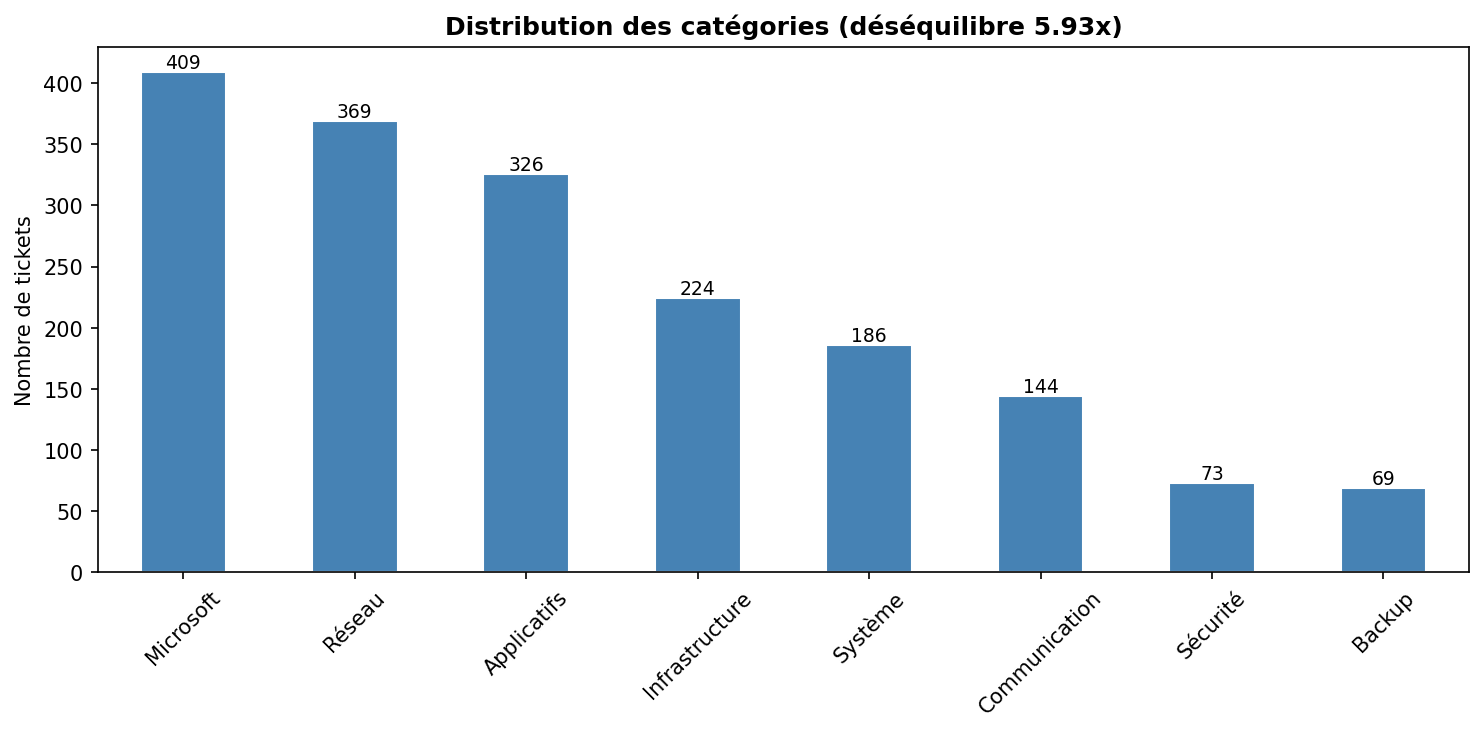
\includegraphics[width=0.94\textwidth]{ch03_distribution_categories.png}
\caption{Répartition des tickets par catégorie}
\label{fig:distcat}
\end{figure}

La distribution de la figure~\ref{fig:distcat} est nettement inégale. \emph{Microsoft} rassemble
409 tickets et \emph{Réseau} 369, quand \emph{Sécurité} en compte 73 et \emph{Backup} 69. Le rapport
entre la catégorie la plus fréquente et la plus rare atteint 5,93, et les trois premières
concentrent 1\,104 tickets, soit 61\,\% du corpus.

Ce déséquilibre est celui de l'activité réelle du service. Il pose une difficulté de modélisation :
un classifieur entraîné sans précaution privilégie les catégories abondantes, affichant une
exactitude globale élevée tout en échouant sur les catégories rares. Le problème est d'autant plus
gênant que \emph{Sécurité} est celle dont une erreur de classement coûte le plus cher.

\subsection{Complétude des champs et longueur des textes}

\label{sec:completude}

Douze des dix-huit champs sont renseignés sur la totalité des lignes, dont les quatre qui portent
l'information exploitée par les modèles : \texttt{Titre}, \texttt{Description}, \texttt{Catégorie}
et \texttt{knowledge Base}. La figure~\ref{fig:completude} donne le taux de remplissage des
dix-huit champs, le tableau~\ref{tab:completude} détaille les six incomplets.

\begin{figure}[!htbp]
\centering
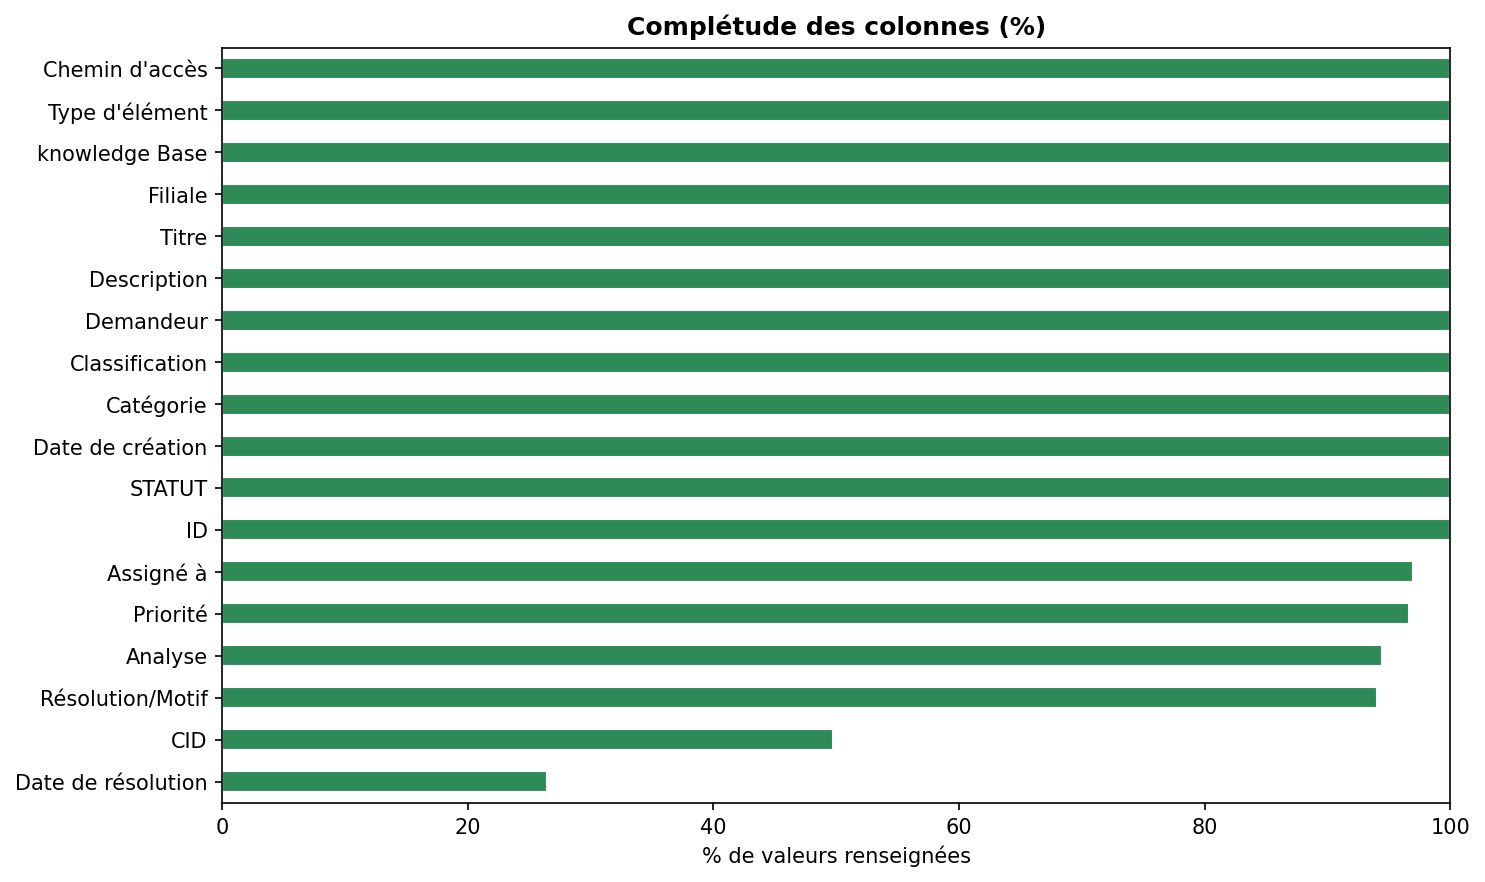
\includegraphics[width=0.92\textwidth]{ch03_completude.png}
\caption{Taux de remplissage des dix-huit champs du jeu de données}
\label{fig:completude}
\end{figure}

\begin{table}[!htbp]
\centering
\styletableau
\caption{Champs incomplets et interprétation}
\label{tab:completude}
\begin{tabular}{|Bp{3.4cm}|Cp{2.0cm}|Lp{7.4cm}|}
\hline
\rowcolor{enteteTab}
\textbf{Champ} & \textbf{Manquant} & \textbf{Interprétation} \\
\hline
\texttt{Date de résolution} & 73,6\,\% & Manquant par construction : seuls les 476 tickets au
statut \emph{Résolu} en portent une \\
\hline
\texttt{CID} & 50,3\,\% & Référence de configuration renseignée au cas par cas, sans caractère
obligatoire \\
\hline
\texttt{Résolution/Motif} & 5,9\,\% & Texte de clôture, qu'aucune règle de saisie n'impose \\
\hline
\texttt{Analyse} & 5,6\,\% & Champ de commentaire libre, facultatif \\
\hline
\texttt{Priorité} & 3,4\,\% & Non renseignée à la saisie \\
\hline
\texttt{Assigné à} & 3,1\,\% & Tickets non encore attribués au moment de l'export \\
\hline
\end{tabular}
\end{table}

Aucune de ces lacunes ne compromet le projet : les deux taux les plus élevés s'expliquent par la
nature des champs concernés, et les quatre autres restent sous 6\,\%. Le service renseigne
correctement les fiches qu'il traite ; ce qui manque relève du cycle de vie du ticket ou de champs
facultatifs.

Reste à savoir ce que contiennent les champs renseignés. Les descriptions sont courtes et
homogènes : de 23 à 46 mots, pour une médiane de 33, et les titres comptent de 2 à 8 mots. Aucun
ticket n'est vide ni aberrant par la longueur, comme le montre la distribution complète de la
figure~\ref{fig:longueurs}. Cette homogénéité dispense de tronquer ou de segmenter les textes avant
de les soumettre à un transformer.

% Placement [H] : la figure est large et basse, et une barriere de flottants lui
% laissait une page entiere. Ancree ici, elle suit le texte qui la commente et la
% sous-section suivante enchaine sur la meme page.
\begin{figure}[H]
\centering
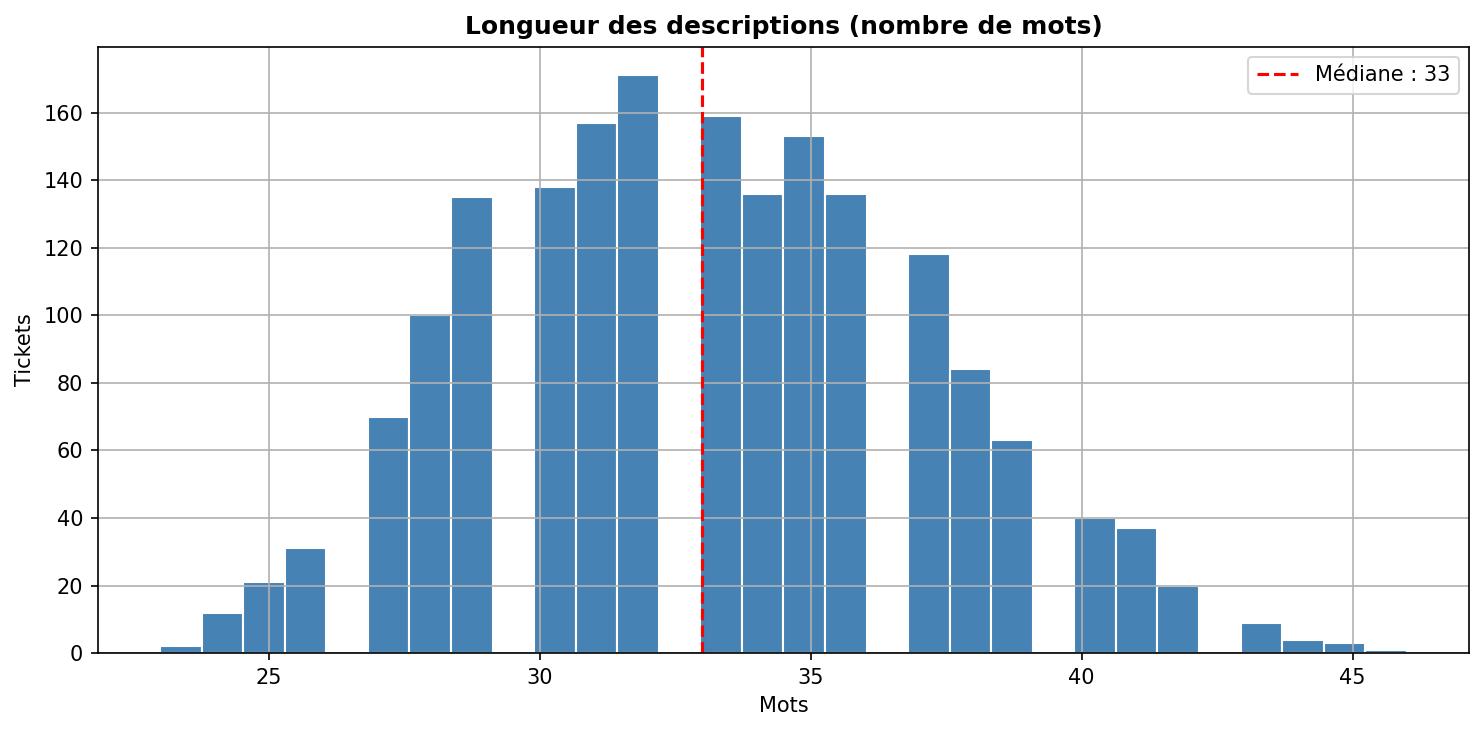
\includegraphics[width=0.86\textwidth]{ch03_longueurs.png}
\caption{Distribution de la longueur des descriptions, en nombre de mots}
\label{fig:longueurs}
\end{figure}

\subsection{Statuts, délais et décomptes du corpus}

\begin{table}[!htbp]
\centering
\styletableau
\caption{Répartition des tickets par statut}
\label{tab:statuts}
\begin{tabular}{|Bp{4.0cm}|Cp{2.4cm}|Cp{2.4cm}|}
\hline
\rowcolor{enteteTab}
\textbf{Statut} & \textbf{Tickets} & \textbf{Part} \\
\hline
Résolu & 476 & 26,4\,\% \\
\hline
Rejeté & 464 & 25,8\,\% \\
\hline
Problème & 328 & 18,2\,\% \\
\hline
Prise en charge & 321 & 17,8\,\% \\
\hline
En attente & 211 & 11,7\,\% \\
\hline
\end{tabular}
\end{table}

Le champ \texttt{STATUT} décrit l'état du ticket au moment de l'export
(tableau~\ref{tab:statuts}). Le taux de rejet qu'il fait apparaître a été commenté au chapitre~1 ;
ce que la répartition apporte ici est une limite de mesure. Les 476 tickets résolus sont les seuls
à porter une date de résolution, ce qui restreint tout calcul de délai à 26,4\,\% du corpus. Sur ce
sous-ensemble, le délai médian entre création et résolution s'établit à deux jours, avec un maximum
de quatre. La charge réelle du service reste hors de portée.

\textbf{Trois décomptes à ne pas confondre.} Le reste du mémoire distingue trois ensembles que
le langage courant réunit sous le même mot, et s'y tient.

\begin{puces}
\item Les \textbf{tickets historiques} sont les 1\,800 lignes de l'export, quel que soit leur
statut. C'est le corpus, et c'est à lui que renvoie tout chiffre global.
\item Les \textbf{tickets résolus} sont les 476 lignes au statut \emph{Résolu}, soit 26,4\,\% du
corpus. Eux seuls portent une date de résolution, et eux seuls alimentent la collecte de
réapprentissage décrite au chapitre~7.
\item Les \textbf{tickets documentés} sont les 1\,693 lignes dont le champ
\texttt{Résolution\,/\,Motif} porte un texte, soit 94,1\,\% du corpus. Un refus motivé, un
diagnostic posé ou un blocage décrit en font partie. C'est de cet ensemble, et non des seuls
tickets résolus, que la base de connaissances du chapitre~5 est tirée.
\end{puces}

Le recouvrement est partiel dans les deux sens : 26 tickets résolus ne portent aucun texte de
résolution, et 1\,243 tickets documentés n'ont pas le statut \emph{Résolu}. Parler de
« 1\,800 tickets résolus » serait donc inexact deux fois plutôt qu'une.

\subsection{Redondance du corpus}

Un corpus peut compter beaucoup de lignes sans porter beaucoup de situations distinctes.
Trois dénombrements suffisent à mesurer cet écart.

\begin{figure}[!htbp]
\centering
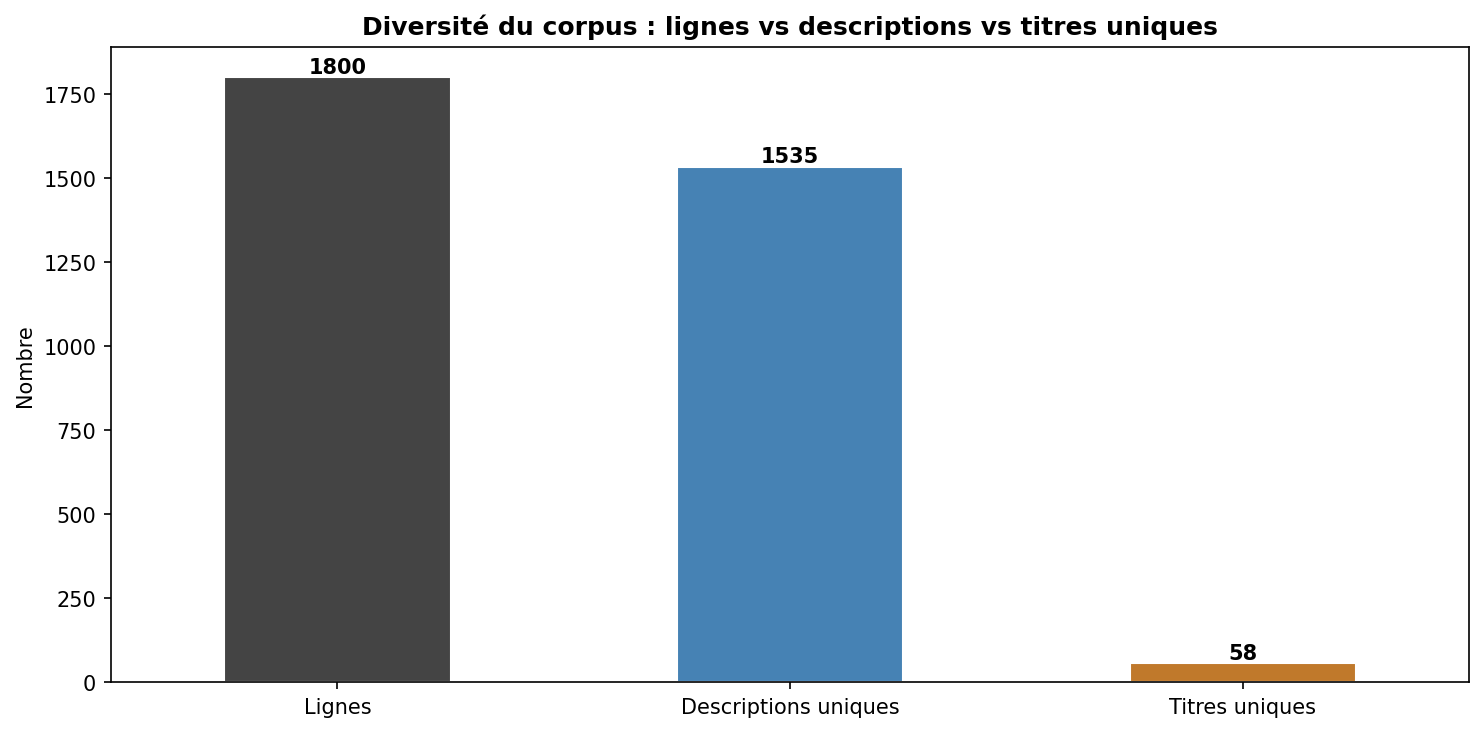
\includegraphics[width=0.90\textwidth]{ch03_redondance.png}
\caption{Diversité du corpus : lignes, descriptions et titres distincts}
\label{fig:redondance}
\end{figure}

La figure~\ref{fig:redondance} les rapproche. Pour 1\,800 lignes, nous dénombrons
1\,535 descriptions distinctes, soit 85\,\%. Les titres ne prennent que 58 valeurs distinctes, et le
champ \texttt{knowledge Base} en prend exactement autant. Le corpus s'organise donc autour de
58 types de tickets récurrents, chacun instancié en moyenne 31 fois avec des variations de surface :
demandeur, dates, identifiants de configuration, tournures de phrase.

La conséquence porte sur le protocole expérimental. Un découpage aléatoire placerait le même type de
ticket des deux côtés ; le modèle retrouverait au test un scénario déjà vu, et le score mesuré
refléterait sa capacité à mémoriser plutôt qu'à généraliser.

\section{Diagnostic de qualité et risques}

Les quatre analyses qui précèdent portent chacune sur un aspect du corpus. Cette section les
rassemble en un diagnostic unique, puis nomme les risques que ce diagnostic fait peser sur la suite
du travail et le traitement retenu pour chacun.

\subsection{Synthèse du diagnostic}

Les indicateurs du tableau~\ref{tab:dq} proviennent tous du script de diagnostic exécuté sur le
corpus, qui écrit ses résultats dans un fichier de métriques et engendre les figures de cette
section. Aucune valeur n'a été saisie à la main, ce qui rend le diagnostic reproductible à
l'identique.

\begin{table}[!htbp]
\centering
\styletableau
\caption{Synthèse du diagnostic de qualité}
\label{tab:dq}
\begin{tabular}{|Bp{5.0cm}|Lp{3.6cm}|Lp{4.2cm}|}
\hline
\rowcolor{enteteTab}
\textbf{Indicateur} & \textbf{Valeur} & \textbf{Lecture} \\
\hline
Lignes et champs & 1\,800 sur 18 champs & Volume exploitable \\
\hline
Catégories & 8 & Classification multi-classes \\
\hline
Déséquilibre maximal & 5,93 & À traiter en modélisation \\
\hline
Tickets vides & 0 & Aucun \\
\hline
Doublons de ligne complète & 0 & Aucun \\
\hline
Incohérences d'étiquetage & 0 & Annotation fiable \\
\hline
Descriptions distinctes & 1\,535 sur 1\,800 & Diversité satisfaisante \\
\hline
Titres distincts & 58 & Corpus organisé par scénarios \\
\hline
Longueur des descriptions & médiane 33 mots & Textes homogènes \\
\hline
Champs critiques manquants & 0 & Complétude assurée \\
\hline
\end{tabular}
\end{table}

Le corpus est structurellement sain. Ses difficultés portent sur la forme de sa distribution et sur
sa composition ; son intégrité est acquise.

\subsection{Risques identifiés et traitements retenus}

Le diagnostic qui précède fait apparaître des risques pour l'apprentissage. Le
tableau~\ref{tab:risques} associe à chacun son effet attendu sur les modèles et le traitement
décidé.

\begin{table}[!htbp]
\centering
\styletableau
\caption{Risques liés aux données et traitements associés}
\label{tab:risques}
\begin{tabular}{|Bp{3.2cm}|Lp{4.4cm}|Lp{5.2cm}|}
\hline
\rowcolor{enteteTab}
\textbf{Risque} & \textbf{Effet attendu} & \textbf{Traitement} \\
\hline
Déséquilibre des catégories & Rappel faible sur \emph{Sécurité} et \emph{Backup} & Métrique
F1-macro, pondération des classes, suivi du rappel par classe (chapitre~4) \\
\hline
Redondance des types de tickets & Fuite entre entraînement et test, scores surestimés & Découpage
par groupe de titres (section~\ref{sec:antifuite}) \\
\hline
Nettoyage trop agressif & Perte de signal lexical, généralisation dégradée & Révision des règles,
conservation du vocabulaire informatique \\
\hline
Champs incomplets & Base de connaissances lacunaire & Repli de \texttt{Résolution/Motif} sur
\texttt{knowledge Base} (chapitre~5) \\
\hline
Données personnelles en clair & Exposition de noms et de rattachements & Pseudonymisation par
empreinte à clé (chapitre~6) \\
\hline
\end{tabular}
\end{table}

\section{Limites du corpus}

\label{sec:representativite}

La section précédente traitait de risques que nous avons pu corriger. Celle-ci énonce une
limite que nous n'avons pas les moyens de lever : le corpus décrit fidèlement l'activité du service
support d'\OTBS sur quatorze mois, et rien de plus.

Sa composition en 58 scénarios récurrents en délimite la portée. Un modèle entraîné sur ces données
apprend à reconnaître des familles de problèmes déjà rencontrées ; le corpus ne permet pas de
mesurer sa capacité à traiter un problème inédit, faute d'y trouver de tels cas. Les performances
du chapitre~6 doivent se lire à cette échelle.

Deux restrictions de périmètre s'y ajoutent. Le corpus couvre les huit filiales du groupe et leur
parc applicatif, si bien que les résultats ne se transposent pas à une organisation dont le paysage
informatique diffère. Le référentiel de huit catégories est propre au service : un autre découpage
métier produirait un autre problème de classification.


% Aucun flottant du corps ne doit franchir la conclusion.
\FloatBarrier

\section*{Conclusion}
\addcontentsline{toc}{section}{Conclusion}

Le corpus est maintenant connu. Il compte 1\,800 tickets créés sur quatorze mois, décrits par
dix-huit champs dont quatre portent l'information exploitable. Sa distribution est inégale, la
catégorie la plus fréquente dépassant la plus rare d'un facteur 5,93.

Le constat déterminant est ailleurs. Pour 1\,800 lignes, le corpus ne porte que cinquante-huit
titres distincts, contre 1\,535 descriptions différentes. Le chapitre~1 lisait cet écart comme le
symptôme d'un travail répétitif ; mesuré ici, il devient une contrainte expérimentale, car tout
découpage qui ignore les titres mesurerait la mémorisation plutôt que la généralisation.

Les risques que ce diagnostic fait peser sont énoncés avec le traitement retenu pour chacun. Le
chapitre suivant ouvre la troisième phase et met ces traitements en œuvre.

        \clearpage

        \chapter{Sprint 1 --- Données et gouvernance}

\section*{Introduction}
\addcontentsline{toc}{section}{Introduction}

Avant d'entraîner un modèle, il faut connaître les données sur lesquelles il apprendra. Le premier
sprint a donc porté sur le corpus : le rassembler, le décrire, mesurer ce qu'il vaut, puis le
préparer.

Nous présentons ici ce corpus : sa provenance, son contenu, ce que son analyse a révélé, les
corrections que nous lui avons apportées et les limites qui subsistent. La dernière section traite
du découpage entre entraînement et test. Elle occupe une place importante dans ce chapitre, car la
validité de tous les résultats rapportés aux chapitres~4 et~5 en dépend.

\section{Objectifs du sprint}

Le sprint poursuit cinq objectifs, récapitulés au tableau~\ref{tab:obj3}. Ils suivent le
séquencement de CRISP-DM exposé au chapitre~1 : comprendre les données avant de les préparer, et
les préparer avant d'entraîner quoi que ce soit.

\begin{table}[!htbp]
\centering
\styletableau
\caption{Objectifs du sprint 1 et livrables associés}
\label{tab:obj3}
\begin{tabular}{|Cp{0.8cm}|Lp{6.0cm}|Lp{4.4cm}|Lp{2.4cm}|}
\hline
\rowcolor{enteteTab}
\textbf{N\textsuperscript{o}} & \textbf{Objectif} & \textbf{Livrable} & \textbf{État} \\
\hline
1 & Décrire le corpus et mesurer sa qualité & Rapport de diagnostic et figures associées &
Atteint \\
\hline
2 & Situer le corpus par rapport à un jeu de données public & Comparaison structurelle et
lexicale & Atteint \\
\hline
3 & Définir des règles de nettoyage adaptées au vocabulaire informatique & Module de
prétraitement & Atteint \\
\hline
4 & Établir un découpage entraînement/test exempt de fuite & Jeux \texttt{train}, \texttt{test} et
\texttt{rag} & Atteint avec réserve \\
\hline
5 & Rendre la préparation reproductible & Pipeline de données versionné & Atteint \\
\hline
\end{tabular}
\end{table}

La réserve portée à l'objectif~4 s'explique à la section~\ref{sec:composition}. Le découpage
élimine bien la fuite que nous cherchions à supprimer, mais il produit un jeu de test dont la
couverture reste incomplète. Le protocole d'évaluation du chapitre~4 tient compte de ce défaut.

\section{Le jeu de données}

\subsection{Provenance et mode de collecte}

Le corpus provient de la liste SharePoint tenue par le service support, exportée au format CSV. Le
champ \texttt{Chemin d'accès} conserve l'emplacement d'origine de chaque enregistrement,
\texttt{sites/IT-Check/Lists/HelpDesk}, ce qui atteste la provenance sans dépendre d'une
déclaration.

L'export compte 1\,800 tickets créés entre le 1\textsuperscript{er} janvier 2025 et le
17 février 2026, soit quatorze mois d'activité et une moyenne de 129 tickets par mois. Ils émanent
de 202 demandeurs distincts répartis sur les huit filiales du groupe, et sont assignés à onze
intervenants, ce qui recoupe l'effectif du service décrit au chapitre~1.

Un défaut de saisie se voit dès l'ouverture du fichier. Le champ \texttt{Date de création} mélange
deux formats : 828 lignes au format ISO \texttt{AAAA-MM-JJ hh:mm:ss} et 972 au format français
\texttt{JJ/MM/AAAA hh:mm}. Une lecture qui n'essaierait qu'un seul format écarterait silencieusement
plus de la moitié des dates et fausserait toute statistique temporelle. Nous reconnaissons donc les
deux formats explicitement au chargement.

\subsection{Schéma et variable cible}

Chaque ticket est décrit par dix-huit champs. Le tableau~\ref{tab:schema} les regroupe par rôle
plutôt que dans l'ordre du fichier, afin de faire apparaître la structure de l'information.

\begin{table}[!htbp]
\centering
\styletableau
\caption{Organisation des dix-huit champs du jeu de données}
\label{tab:schema}
\begin{tabular}{|Bp{2.6cm}|Lp{5.2cm}|Lp{5.8cm}|}
\hline
\rowcolor{enteteTab}
\textbf{Groupe} & \textbf{Champs} & \textbf{Rôle dans le projet} \\
\hline
Identification & \texttt{ID}, \texttt{CID} & Clé du ticket et référence de configuration \\
\hline
Contenu & \texttt{Titre}, \texttt{Description} & Entrée textuelle des modèles \\
\hline
Classement & \texttt{Catégorie}, \texttt{Classification}, \texttt{Priorité} & \texttt{Catégorie}
est la variable cible ; les deux autres servent de contexte \\
\hline
Acteurs & \texttt{Demandeur}, \texttt{Filiale}, \texttt{Assigné~à} & Traçabilité de la demande et
de son traitement \\
\hline
Suivi & \texttt{STATUT}, \texttt{Date de création}, \texttt{Date de résolution} & Cycle de vie du
ticket \\
\hline
Résolution & \texttt{Résolution/Motif}, \texttt{Analyse}, \texttt{knowledge Base} & Matière de la
base de connaissances interrogée par le moteur RAG \\
\hline
Provenance & \texttt{Type d'élément}, \texttt{Chemin~d'accès} & Origine SharePoint de
l'enregistrement \\
\hline
\end{tabular}
\end{table}

La variable cible est le champ \texttt{Catégorie}, qui prend huit modalités : \emph{Microsoft},
\emph{Réseau}, \emph{Applicatifs}, \emph{Infrastructure}, \emph{Système}, \emph{Communication},
\emph{Sécurité} et \emph{Backup}. C'est le référentiel employé par le service, déjà introduit au
chapitre~1.

L'annotation elle-même est fiable. Aucun titre de ticket ne reçoit deux catégories différentes
selon les enregistrements : sur les 58 libellés distincts que compte le corpus, la correspondance
du titre vers la catégorie est une fonction, sans exception. Ce constat écarte d'emblée le bruit
d'étiquetage comme explication des performances observées au chapitre~4.

\subsection{Un jeu de données public pour situer le corpus}

Pour disposer d'un point de comparaison extérieur, nous avons chargé un jeu de données public de
tickets de support \cite{hfTickets}, filtré sur les enregistrements en langue anglaise, soit
11\,923 tickets décrits par quinze champs. Sa structure recoupe largement la nôtre, comme le montre
le tableau~\ref{tab:bench}.

\begin{table}[!htbp]
\centering
\styletableau
\caption{Correspondance entre le corpus \OTBS et le jeu de données public}
\label{tab:bench}
\begin{tabular}{|Bp{3.6cm}|Lp{4.2cm}|Lp{5.4cm}|}
\hline
\rowcolor{enteteTab}
\textbf{Corpus \OTBS} & \textbf{Jeu public} & \textbf{Rôle} \\
\hline
\texttt{Titre} & \texttt{subject} & Titre court \\
\hline
\texttt{Description} & \texttt{body} & Texte libre \\
\hline
\texttt{Catégorie} (8 classes) & \texttt{queue} (10 classes) & Cible de classification \\
\hline
\texttt{Classification} & \texttt{type} & Nature de la demande \\
\hline
\texttt{Priorité} & \texttt{priority} & Priorité déclarée \\
\hline
\texttt{Résolution/Motif} & \texttt{answer} & Réponse apportée \\
\hline
\end{tabular}
\end{table}

La langue et le domaine applicatif diffèrent trop pour que ce jeu serve à l'entraînement. Il sert
de repère, et livre au passage un chiffre réexploité plus loin. Le jeu public compte 10\,891 titres
distincts pour 11\,923 tickets, soit 91\,\% de titres uniques. Le nôtre en compte 58 pour 1\,800, soit 3\,\%. L'écart est
considérable pour deux corpus qui décrivent la même activité ; nous y revenons à la
section~\ref{sec:representativite}.

\section{Analyse exploratoire}

\subsection{Distribution des catégories}

La figure~\ref{fig:distcat} donne la répartition des 1\,800 tickets entre les huit catégories.

\begin{figure}[!htbp]
\centering
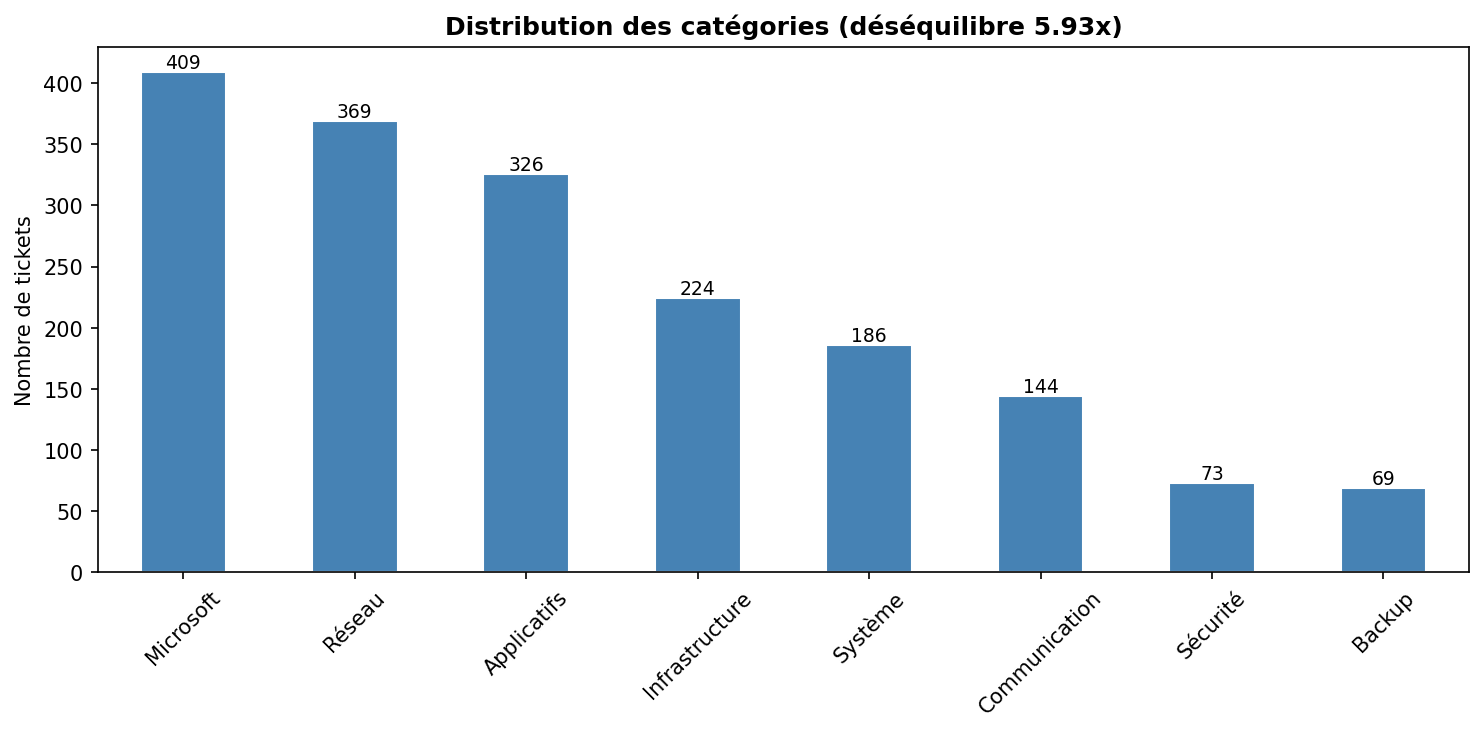
\includegraphics[width=0.94\textwidth]{ch03_distribution_categories.png}
\caption{Répartition des tickets par catégorie}
\label{fig:distcat}
\end{figure}

La distribution est nettement inégale. \emph{Microsoft} rassemble 409 tickets et \emph{Réseau} 369,
quand \emph{Sécurité} en compte 73 et \emph{Backup} 69. Le rapport entre la catégorie la plus
fréquente et la plus rare atteint 5,93. Les trois premières catégories concentrent à elles seules
1\,104 tickets, soit 61\,\% du corpus.

Ce déséquilibre est celui de l'activité réelle du service. Il pose en revanche une difficulté de
modélisation. Un classifieur entraîné sans précaution sur une telle
distribution apprend à privilégier les catégories abondantes ; il affiche alors une exactitude
globale élevée tout en échouant sur les catégories rares. Le problème est d'autant plus gênant que
\emph{Sécurité}, l'une des deux catégories les moins représentées, est celle dont une erreur de
classement coûte le plus cher au service. Nous traitons ce point au chapitre~4, par le choix de la
métrique et par la pondération des classes.

\subsection{Complétude des champs}

Douze des dix-huit champs sont renseignés sur la totalité des lignes, dont les quatre qui portent
l'information exploitée par les modèles : \texttt{Titre}, \texttt{Description}, \texttt{Catégorie}
et \texttt{knowledge Base}. Le tableau~\ref{tab:completude} recense les six champs incomplets.

\begin{table}[!htbp]
\centering
\styletableau
\caption{Champs incomplets et interprétation}
\label{tab:completude}
\begin{tabular}{|Bp{3.4cm}|Cp{2.0cm}|Lp{7.4cm}|}
\hline
\rowcolor{enteteTab}
\textbf{Champ} & \textbf{Manquant} & \textbf{Interprétation} \\
\hline
\texttt{Date de résolution} & 73,6\,\% & Manquant par construction : seuls les 476 tickets au
statut \emph{Résolu} en portent une \\
\hline
\texttt{CID} & 50,3\,\% & Référence de configuration renseignée au cas par cas, sans caractère
obligatoire \\
\hline
\texttt{Résolution/Motif} & 5,9\,\% & Traité par un repli sur \texttt{knowledge Base} dans le
moteur RAG \\
\hline
\texttt{Analyse} & 5,6\,\% & Champ de commentaire libre, facultatif \\
\hline
\texttt{Priorité} & 3,4\,\% & Non renseignée à la saisie \\
\hline
\texttt{Assigné à} & 3,1\,\% & Tickets non encore attribués au moment de l'export \\
\hline
\end{tabular}
\end{table}

Aucune de ces lacunes ne compromet le projet. Les deux taux les plus élevés s'expliquent par la
nature même des champs concernés, et les quatre autres restent sous 6\,\%. Le diagnostic du
chapitre~1 s'éclaire au passage : les canaux d'arrivée hétérogènes dégradaient la traçabilité en
amont de la liste SharePoint, mais le service remplissait correctement les enregistrements qui y
parvenaient.

\subsection{Longueur des textes et cycle de vie}

Les descriptions sont courtes et homogènes : de 23 à 46 mots, pour une médiane de 33 et une moyenne
de 33,1. Aucun ticket n'est vide, aucun n'est aberrant par la longueur. Les titres comptent de 2 à
8 mots, avec une médiane de 5. Cette homogénéité facilite la modélisation, puisqu'elle dispense de
tronquer ou de segmenter les textes avant de les soumettre à un transformer.

Le champ \texttt{STATUT} décrit l'état du ticket au moment de l'export. Sa distribution figure au
tableau~\ref{tab:statuts}.

\begin{table}[!htbp]
\centering
\styletableau
\caption{Répartition des tickets par statut}
\label{tab:statuts}
\begin{tabular}{|Bp{4.0cm}|Cp{2.4cm}|Cp{2.4cm}|}
\hline
\rowcolor{enteteTab}
\textbf{Statut} & \textbf{Tickets} & \textbf{Part} \\
\hline
Résolu & 476 & 26,4\,\% \\
\hline
Rejeté & 464 & 25,8\,\% \\
\hline
Problème & 328 & 18,2\,\% \\
\hline
Prise en charge & 321 & 17,8\,\% \\
\hline
En attente & 211 & 11,7\,\% \\
\hline
\end{tabular}
\end{table}

Le taux de rejet frappe d'abord : 464 tickets, soit plus d'un quart du corpus, ont été
écartés sans résolution. Le chapitre~1 avait relevé ce point comme un symptôme de l'absence de
qualification à l'entrée, une demande mal formulée ou mal orientée occupant un consultant avant
d'être rejetée.

Les tickets clos posent un problème différent, un problème de mesure. Les 476 tickets
résolus sont les seuls à porter une date de résolution, ce qui restreint tout calcul de délai à
26,4\,\% du corpus. Sur ce sous-ensemble, le délai médian entre création et résolution s'établit à
deux jours, avec un maximum de quatre. Cette valeur vaut pour les seuls tickets menés à leur terme
et laisse hors champ ceux qui sont restés ouverts ou ont été rejetés ; la charge du service reste
donc hors de sa portée.

\subsection{Redondance du corpus}

Reste à mesurer la diversité réelle du corpus. La figure~\ref{fig:redondance} rapproche trois
décomptes.

\begin{figure}[!htbp]
\centering
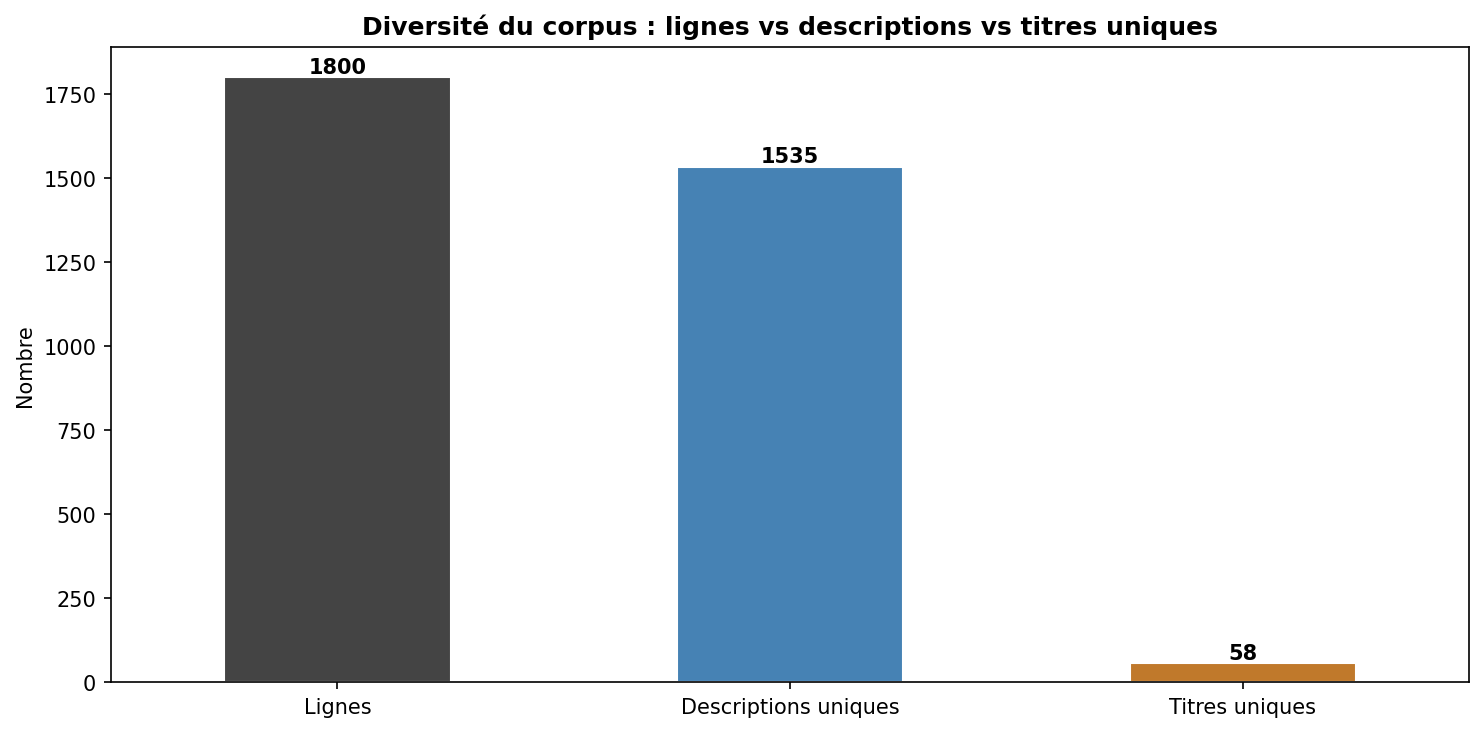
\includegraphics[width=0.90\textwidth]{ch03_redondance.png}
\caption{Diversité du corpus : lignes, descriptions et titres distincts}
\label{fig:redondance}
\end{figure}

Pour 1\,800 lignes, nous dénombrons 1\,535 descriptions distinctes, soit 85\,\% : à ce niveau, la
diversité est bonne. Les titres, eux, ne prennent que 58 valeurs distinctes, et le champ
\texttt{knowledge Base} en prend exactement autant. Le corpus s'organise donc autour de 58 types de
tickets récurrents, chacun instancié en moyenne 31 fois avec des variations de surface : demandeur,
dates, identifiants de configuration, tournures de phrase.

Cette structure a une conséquence directe sur le protocole expérimental. Un découpage aléatoire
entre entraînement et test placerait le même type de ticket des deux côtés. Le modèle retrouverait
au test un scénario déjà vu à l'entraînement, et le score mesuré refléterait sa capacité à mémoriser
plutôt qu'à généraliser. La section~\ref{sec:antifuite} traite ce risque.

\section{Diagnostic de qualité des données}

\subsection{Synthèse des indicateurs}

Le tableau~\ref{tab:dq} rassemble les indicateurs calculés dans les sections précédentes.

\begin{table}[!htbp]
\centering
\styletableau
\caption{Synthèse du diagnostic de qualité}
\label{tab:dq}
\begin{tabular}{|Bp{5.0cm}|Lp{3.6cm}|Lp{4.2cm}|}
\hline
\rowcolor{enteteTab}
\textbf{Indicateur} & \textbf{Valeur} & \textbf{Lecture} \\
\hline
Lignes et champs & 1\,800 sur 18 champs & Volume exploitable \\
\hline
Catégories & 8 & Classification multi-classes \\
\hline
Déséquilibre maximal & 5,93 & À traiter en modélisation \\
\hline
Tickets vides & 0 & Aucun \\
\hline
Doublons de ligne complète & 0 & Aucun \\
\hline
Incohérences d'étiquetage & 0 & Annotation fiable \\
\hline
Descriptions distinctes & 1\,535 sur 1\,800 & Diversité satisfaisante \\
\hline
Titres distincts & 58 & Corpus organisé par scénarios \\
\hline
Longueur des descriptions & médiane 33 mots & Textes homogènes \\
\hline
Champs critiques manquants & 0 & Complétude assurée \\
\hline
\end{tabular}
\end{table}

Le corpus est structurellement sain : aucune ligne vide, aucun doublon, aucune contradiction
d'étiquetage, et une complétude totale sur les champs essentiels. Ses difficultés portent sur la
forme de sa distribution et sur sa composition ; son intégrité, elle, est acquise.

\subsection{Risques identifiés et traitements retenus}

Le tableau~\ref{tab:risques} associe à chaque risque son effet attendu sur les modèles et le
traitement décidé, avec l'endroit du mémoire où ce traitement est mis en œuvre.

\begin{table}[!htbp]
\centering
\styletableau
\caption{Risques liés aux données et traitements associés}
\label{tab:risques}
\begin{tabular}{|Bp{2.9cm}|Lp{3.8cm}|Lp{4.2cm}|Cp{1.5cm}|}
\hline
\rowcolor{enteteTab}
\textbf{Risque} & \textbf{Effet attendu} & \textbf{Traitement} & \textbf{Où} \\
\hline
Déséquilibre des catégories & Rappel faible sur \emph{Sécurité} et \emph{Backup} & Métrique
F1-macro, pondération des classes, suivi du rappel par classe & Ch.~4 \\
\hline
Redondance des types de tickets & Fuite entre entraînement et test, scores surestimés & Découpage
par groupe de titres & \S\ref{sec:antifuite} \\
\hline
Nettoyage trop agressif & Perte de signal lexical, généralisation dégradée & Révision des règles,
conservation du vocabulaire informatique & \S\ref{sec:nettoyage} \\
\hline
Champs incomplets & Base de connaissances lacunaire & Repli de \texttt{Résolution/Motif} sur
\texttt{knowledge Base} & Ch.~5 \\
\hline
Données personnelles en clair & Exposition de noms et de rattachements & Non traité &
\S\ref{sec:rgpd} \\
\hline
\end{tabular}
\end{table}

\subsection{Limite assumée : la représentativité du corpus}
\label{sec:representativite}

Les deux sous-sections précédentes traitaient de risques que nous avons pu corriger. Celle-ci
énonce une limite que nous n'avons pas les moyens de lever. Le corpus décrit fidèlement l'activité
du service support d'\OTBS sur quatorze mois, et rien de plus.

Sa composition en 58 scénarios récurrents en délimite la portée. Un modèle entraîné sur ces données
apprend à reconnaître des familles de problèmes déjà rencontrées ; en revanche, ce corpus ne permet
pas de mesurer sa capacité à traiter un problème véritablement inédit, faute d'y trouver de tels
cas. Le rapprochement avec le jeu de données public conduit au même constat par un autre chemin :
91\,\% de titres uniques d'un côté, 3\,\% de l'autre. Les performances rapportées au chapitre~4
doivent se lire à cette échelle.

Le périmètre appelle deux restrictions supplémentaires. Le corpus couvre les huit entités du groupe
et leur parc applicatif, si bien que les résultats ne se transposent pas tels quels à une
organisation dont le paysage informatique diffère. Le référentiel de huit catégories, lui, est
propre au service : un autre découpage métier produirait un autre problème de classification. La
solution garde toute son utilité pour \OTBS, qui en est le destinataire ; ses chiffres, en
revanche, ne se généralisent pas.

\section{Préparation des données}

\subsection{Nettoyage textuel}
\label{sec:nettoyage}

Le nettoyage transforme le texte brut en une chaîne exploitable par les modèles. Il applique
successivement le passage en minuscules, la normalisation Unicode avec suppression des accents, le
retrait des adresses électroniques, des URL et des adresses IP, la suppression de la ponctuation, le
retrait des mots vides et le rejet des unités d'un seul caractère.

Notre première version de ces règles était trop agressive. Si elle figure ici, c'est parce qu'elle
illustre un piège courant. Elle retirait, en plus des mots vides du français et de l'anglais,
une longue liste de termes jugés génériques : \emph{problème}, \emph{système}, \emph{service},
\emph{demande}, \emph{ticket}. Le diagnostic a montré que la description moyenne tombait alors de
33 mots à une douzaine, et la diversité lexicale du corpus à environ 125 motifs distincts. Une
partie de l'uniformité que nous croyions lire dans les données venait en réalité du prétraitement
lui-même.

Nous avons donc révisé les règles. Une trentaine de termes informatiques discriminants sont
désormais protégés du retrait, qu'ils figurent ou non dans les listes de mots vides standard :
\emph{réseau}, \emph{serveur}, \emph{connexion}, \emph{outlook}, \emph{vpn}, \emph{dns},
\emph{sauvegarde}, \emph{sécurité}, entre autres. Les chiffres sont conservés, car un code d'erreur
ou un numéro de version porte de l'information ; seules les adresses IP restent retirées, trop
spécifiques pour se généraliser. La vectorisation retient enfin les unigrammes et les bigrammes, de
manière à capter des expressions comme \og salle serveur \fg{} ou \og tentatives connexion \fg{} que
le découpage en mots isolés dissout.

L'effet de cette révision sur les performances est mesuré au chapitre~4, sous le protocole qui y est
défini.

\subsection{Variables construites}

Nous ajoutons cinq variables aux dix-huit champs d'origine, ce qui porte le jeu préparé à
vingt-trois colonnes. Le tableau~\ref{tab:variables} les décrit.

\begin{table}[!htbp]
\centering
\styletableau
\caption{Variables construites lors de la préparation}
\label{tab:variables}
\begin{tabular}{|Bp{4.4cm}|Lp{4.2cm}|Lp{4.2cm}|}
\hline
\rowcolor{enteteTab}
\textbf{Variable} & \textbf{Construction} & \textbf{Destination} \\
\hline
\texttt{text\_clean} & Titre et description nettoyés & Vectorisation TF-IDF \\
\hline
\texttt{text\_enriched} & Préfixe de contexte, puis titre et description & Modèle CamemBERT \\
\hline
\texttt{text\_rag} & Titre, description, résolution et fiche de connaissance & Indexation du moteur
RAG \\
\hline
\texttt{priorite\_simple} & Quatre niveaux ramenés à trois & Contexte de classification \\
\hline
\texttt{classification\_simple} & Cinq types ramenés à trois & Contexte de classification \\
\hline
\end{tabular}
\end{table}

La variable \texttt{text\_enriched} demande un mot d'explication. Elle place devant le texte du
ticket un préfixe court de la forme \texttt{type demande priorite haute}, construit à partir des
deux variables simplifiées. L'idée est de donner au transformer un signal contextuel que le seul
texte libre ne porte pas toujours : une priorité élevée accompagne plus souvent les catégories
\emph{Infrastructure} et \emph{Sécurité} que \emph{Microsoft}. Le regroupement préalable des
modalités, de quatre à trois niveaux de priorité et de cinq à trois types, réduit le nombre de
préfixes possibles et limite la dispersion.

\subsection{Séparation anti-fuite}
\label{sec:antifuite}

La redondance mise en évidence plus haut impose un mode de découpage particulier. Le corpus
s'organisant en 58 types de tickets réinstanciés, un tirage aléatoire ligne à ligne placerait
presque à coup sûr chaque type des deux côtés de la séparation. Le modèle serait alors évalué sur
des scénarios qu'il a déjà vus, et le score obtenu ne mesurerait plus rien d'utile.

Nous regroupons donc les tickets par titre avant de tirer au sort, de sorte que tous les tickets
d'un même type restent du même côté. La figure~\ref{fig:split} oppose les deux approches.

\begin{figure}[!htbp]
\centering
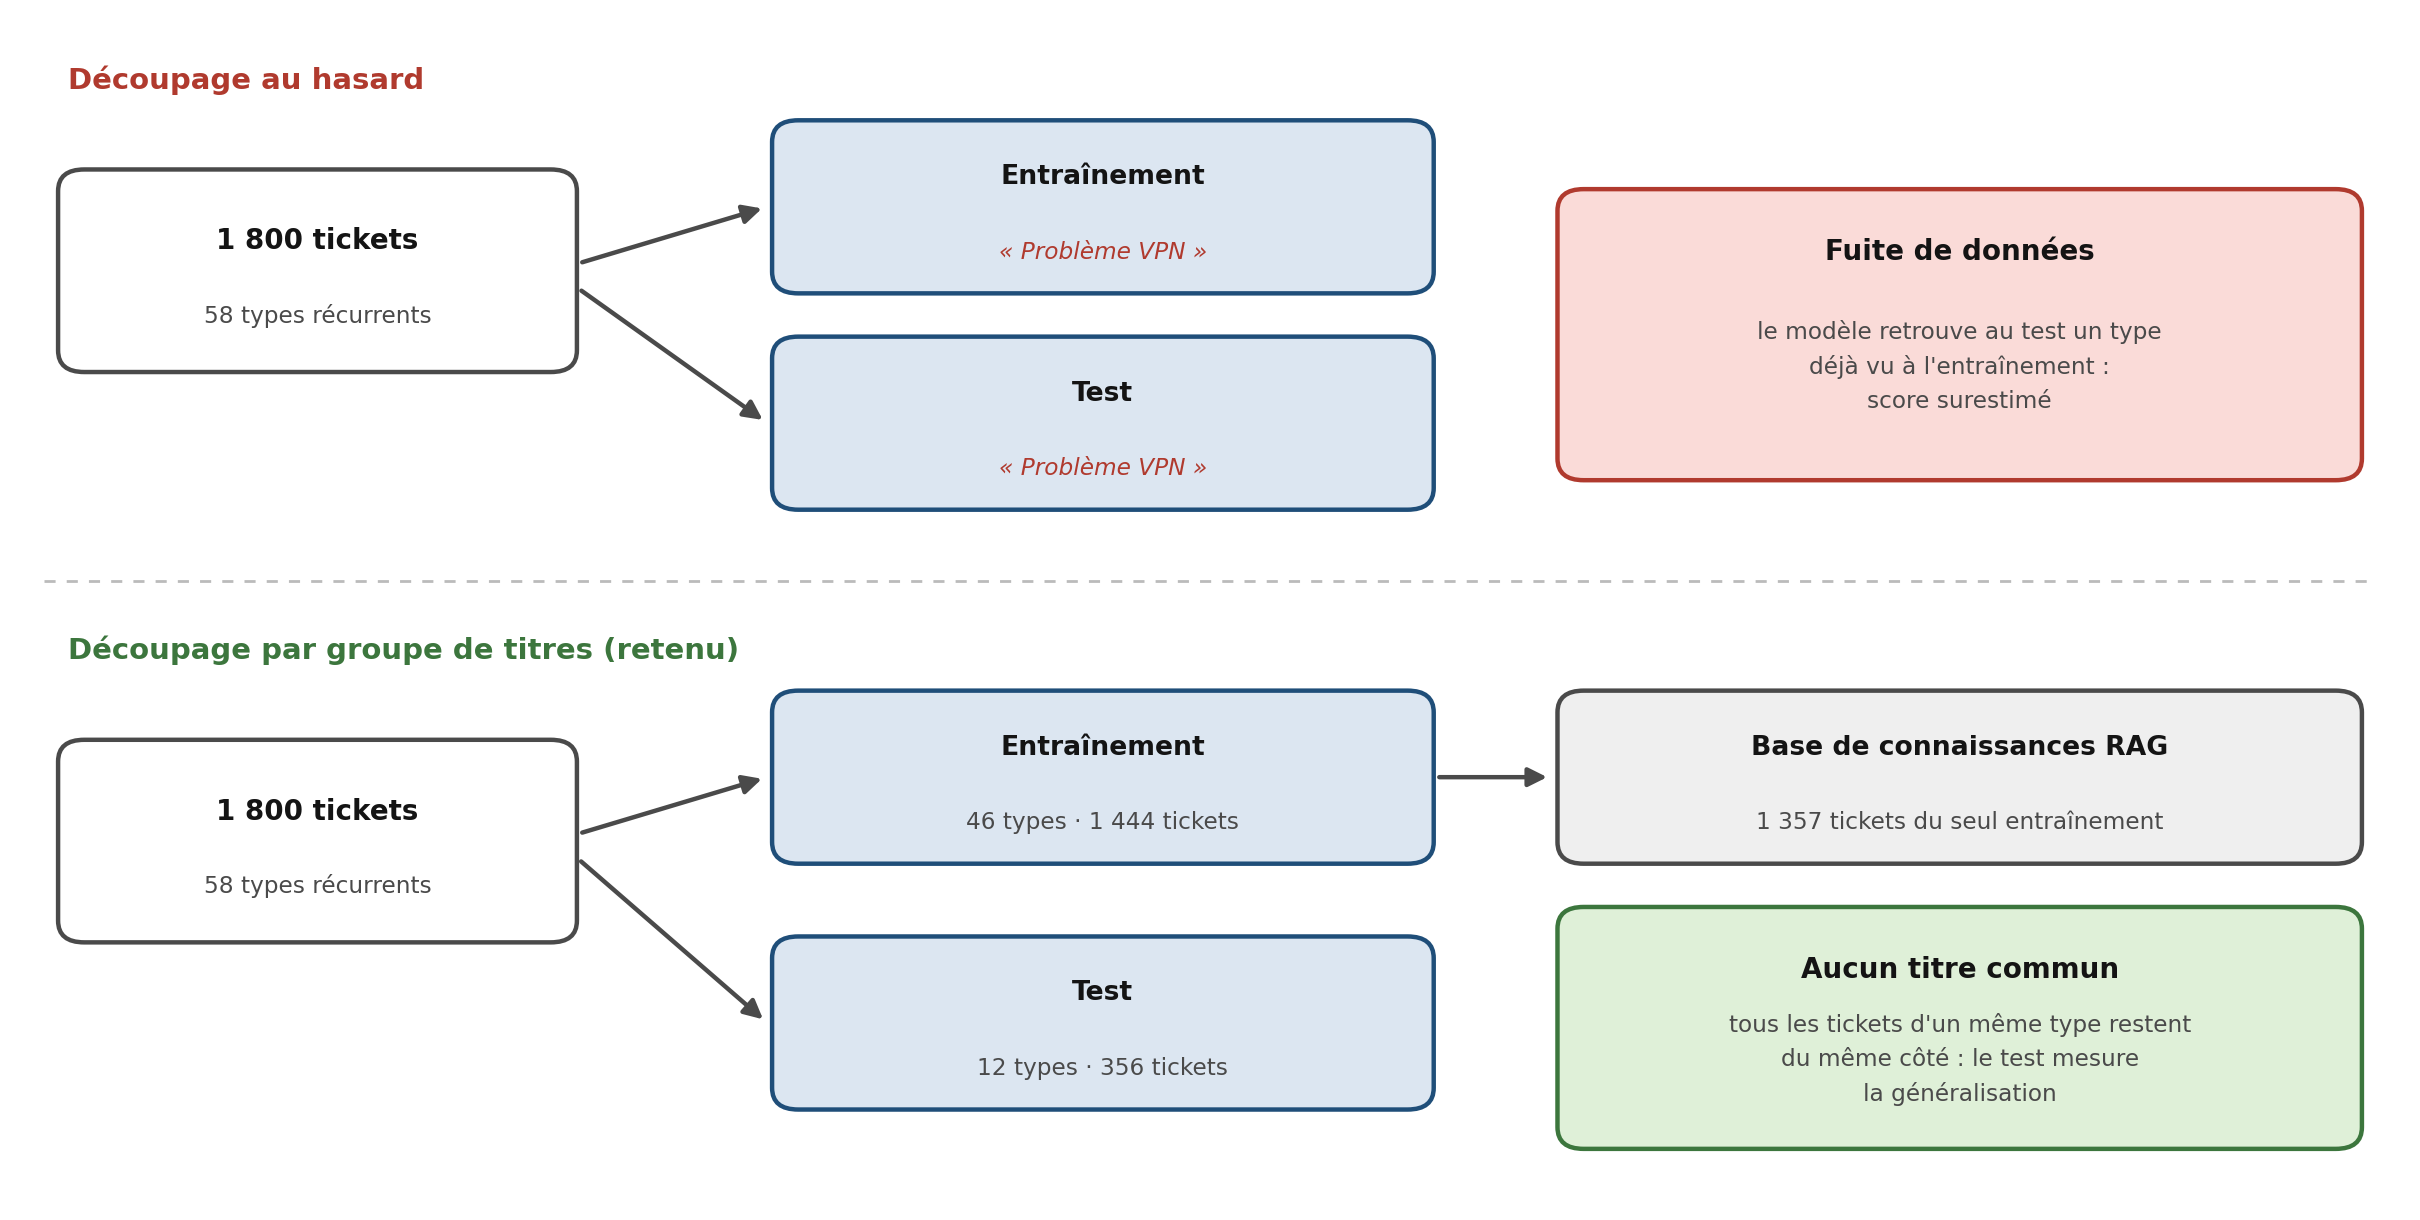
\includegraphics[width=\textwidth]{ch03_split_antifuite.png}
\caption{Découpage aléatoire et découpage par groupe de titres}
\label{fig:split}
\end{figure}

Le tirage est groupé, la colonne \texttt{Titre} servant de variable de groupe, avec une proportion
de test de 20\,\% et une graine aléatoire fixée pour la reproductibilité. Une assertion vérifie
après coup qu'aucun titre n'est commun aux deux jeux et interrompt le traitement dans le cas
contraire. Nous avons préféré cette vérification automatique à une relecture, qui n'aurait protégé
que la première exécution.

La base de connaissances du moteur RAG suit le même principe. Elle ne retient que des tickets du jeu
d'entraînement, ce qui empêche le moteur de retrouver la résolution d'un ticket de test au moment de
l'évaluation. Elle rassemble 1\,357 tickets : tous ceux du jeu d'entraînement
dont le champ \texttt{Résolution/Motif} est renseigné, quel que soit leur statut. Ce dernier point
s'écarte d'une intuition répandue, puisque la base ne se limite pas aux tickets résolus. Nous
l'assumons : un ticket rejeté documente une demande hors périmètre, un ticket en cours documente une
piste d'analyse, et l'un comme l'autre aident un consultant confronté à un cas voisin. La base se
répartit ainsi en 363 tickets rejetés, 358 résolus, 237 au statut \emph{Problème}, 236 pris en
charge et 163 en attente.

\subsection{Composition des jeux obtenus}
\label{sec:composition}

Le découpage produit 1\,444 tickets d'entraînement portant 46 types, et 356 tickets de test portant
les 12 types restants. Aucun titre n'est commun aux deux jeux : la fuite est éliminée.

Le tableau~\ref{tab:splits} donne la composition par catégorie et fait apparaître un effet
secondaire du procédé.

\begin{table}[!htbp]
\centering
\styletableau
\caption{Répartition des catégories dans les jeux obtenus}
\label{tab:splits}
\begin{tabular}{|Bp{3.4cm}|Cp{2.4cm}|Cp{2.2cm}|Cp{2.4cm}|}
\hline
\rowcolor{enteteTab}
\textbf{Catégorie} & \textbf{Entraînement} & \textbf{Test} & \textbf{Base RAG} \\
\hline
Microsoft & 274 & 135 & 263 \\
\hline
Réseau & 324 & 45 & 305 \\
\hline
Applicatifs & 326 & 0 & 303 \\
\hline
Infrastructure & 133 & 91 & 123 \\
\hline
Système & 134 & 52 & 128 \\
\hline
Communication & 144 & 0 & 133 \\
\hline
Sécurité & 40 & 33 & 36 \\
\hline
Backup & 69 & 0 & 66 \\
\hline
\rowcolor{enteteTab}
\textbf{Total} & \textbf{1\,444} & \textbf{356} & \textbf{1\,357} \\
\hline
\end{tabular}
\end{table}

Trois catégories sont absentes du jeu de test : \emph{Applicatifs}, \emph{Communication} et
\emph{Backup}. Le jeu de test ne couvre donc que cinq des huit catégories du référentiel.

Le procédé lui-même produit cet effet. Le tirage porte sur les titres, à l'exclusion des lignes, et
laisse libre la répartition des catégories qui en résulte. Les 12 types tirés au test relèvent
tous de cinq catégories seulement. Rien dans la mécanique du découpage groupé n'empêche cette
configuration, qui devient d'autant plus probable que le nombre de groupes est faible.

La conséquence est directe. Toute moyenne par catégorie calculée sur ce jeu de test porte sur cinq
classes et non sur huit. Le chiffre obtenu est mécaniquement supérieur à celui que donneraient les
huit catégories, puisqu'il exclut du calcul les classes rares, celles-là mêmes que le modèle traite
le moins bien. Les deux valeurs sont exactes ; seule leur comparaison est trompeuse. Le chapitre~4
rapporte donc ses résultats sous un protocole stratifié couvrant les huit catégories, et signale
explicitement les mesures issues du découpage groupé.

Ce constat justifie la réserve portée à l'objectif~4 au tableau~\ref{tab:obj3}. Le découpage remplit
bien la fonction pour laquelle nous l'avions conçu, l'élimination de la fuite ; il introduit en
revanche un biais que nous n'avions pas anticipé. La correction naturelle serait un découpage à la
fois groupé et stratifié, qui préserverait les groupes tout en équilibrant les catégories. Elle
figure parmi les perspectives de la conclusion générale.

\section{Gouvernance et reproductibilité}

\subsection{Versionnement des données et du pipeline}

La préparation décrite dans ce chapitre comporte plusieurs étapes enchaînées, dont les résultats
dépendent de paramètres numériques. Rejouée à la main, elle produirait tôt ou tard un jeu différent
de celui sur lequel les modèles ont été évalués, sans que nous puissions savoir lequel a servi à
quoi.

Nous décrivons donc le pipeline dans un fichier de configuration, exécuté par un outil de
versionnement de données. Le sprint en établit quatre étapes : le prétraitement du fichier brut, le
découpage en jeux, l'entraînement du modèle et la construction de l'index du moteur RAG. Chaque
étape déclare ses dépendances, ses paramètres et ses sorties. L'outil compare les empreintes de ces
éléments avant chaque exécution et ne rejoue que les étapes dont une entrée a changé. Le
chapitre~7 reprend ce même mécanisme et lui ajoute les étapes d'industrialisation.

Les paramètres sont centralisés dans un fichier unique : proportion de test, graine aléatoire,
nombre maximal de descripteurs de la vectorisation, seuils de confiance et de similarité. Les
changer revient à toucher une ligne de configuration plutôt que du code, et l'historique du dépôt
conserve la trace de chaque modification. Les fichiers de données eux-mêmes restent hors du dépôt de
code, remplacés par des empreintes qui permettent de retrouver la version exacte utilisée pour une
mesure donnée.

Le résultat est une garantie précise : chaque chiffre rapporté aux chapitres~4 et~5 se rattache à
une version identifiée des données et à un jeu de paramètres connu, et peut être recalculé à
l'identique.

\subsection{Données personnelles : une limite non traitée}
\label{sec:rgpd}

Le corpus contient des données à caractère personnel. Le champ \texttt{Demandeur} porte les noms de
202 collaborateurs, le champ \texttt{Assigné à} ceux des onze consultants, et le champ
\texttt{Filiale} rattache chaque personne à son entité. Les descriptions mentionnent par ailleurs
des identifiants de postes et de configurations.

Le diagnostic de qualité avait identifié l'anonymisation de ces champs comme une action prioritaire.
Nous ne l'avons pas réalisée. Les traitements décrits dans ce mémoire opèrent sur les données
nominatives telles qu'exportées.

Le manquement est réel, même si deux circonstances en limitent la portée. L'ensemble de la chaîne
s'exécute sur l'infrastructure d'\OTBS, sans transmission vers un service extérieur : l'exigence de
confidentialité posée dès le chapitre~1 est respectée. Et les modèles se nourrissent du seul titre,
de la description et des champs de résolution ; les champs nominatifs restent à l'écart du
traitement. Cela ne nous exonère pas pour autant. Remplacer les noms par des identifiants stables
au moment du chargement aurait coûté peu et supprimé le risque à la source. Le point figure parmi les travaux à conduire
avant tout déploiement élargi.

\section{Bilan du sprint}

Le sprint livre un jeu de données décrit, mesuré, nettoyé, découpé et versionné, ainsi qu'un
diagnostic de qualité qui documente ce que le corpus permet d'établir et ce qu'il ne permet pas.
Les objectifs 1, 2, 3 et 5 sont atteints sans réserve. L'objectif~4, le découpage anti-fuite, l'est
avec la restriction analysée à la section~\ref{sec:composition}.

Trois acquis conditionnent la suite. Le protocole de découpage fixe le cadre d'évaluation de tous
les modèles comparés au chapitre~4. La base de connaissances de 1\,357 tickets fournit la matière du
moteur de recherche construit au chapitre~5. Le troisième est moins visible : le diagnostic de
représentativité, qui détermine par avance l'échelle à laquelle il faudra lire les résultats des
deux chapitres suivants.

\section*{Conclusion}
\addcontentsline{toc}{section}{Conclusion}

Le corpus réuni compte 1\,800 tickets couvrant quatorze mois d'activité, répartis en huit catégories
et décrits par dix-huit champs. Son intégrité est bonne et son annotation cohérente ; les champs
exploités par les modèles sont renseignés partout.

Ses difficultés se situent ailleurs. La distribution des catégories est inégale d'un facteur 5,93,
et le corpus s'organise autour de 58 types de tickets récurrents plutôt qu'autour de problèmes tous
distincts. Le chapitre~4 traite la première, par le choix de la métrique et par la pondération. La
seconde nous a conduits au découpage par groupe de titres : il élimine bien la fuite visée, mais il
laisse trois catégories hors du jeu de test, limite énoncée ici et dont le protocole du chapitre
suivant tient compte.

Le chapitre~4 exploite ces jeux pour comparer plusieurs approches de classification, d'une
vectorisation classique à l'adaptation d'un transformer francophone, et pour analyser les écarts
entre les résultats obtenus et les objectifs fixés au démarrage du projet.

        \clearpage

        \chapter{Sprint 2 --- Modélisation IA}

\section*{Introduction}
\addcontentsline{toc}{section}{Introduction}

Le sprint précédent a livré un corpus décrit, nettoyé et découpé. Celui-ci s'en sert pour construire
le classifieur qui affecte une catégorie à chaque ticket entrant.

Nous avons éprouvé trois approches : une chaîne de vectorisation classique, la même chaîne complétée
par des règles métier, puis l'adaptation d'un transformer francophone. Le chapitre les compare sous
un protocole unique, analyse leurs erreurs et justifie le modèle mis en service.

Autant annoncer d'emblée le résultat principal. La meilleure approche atteint un F1-macro de
0,8343, à 0,016 de l'objectif ENF-03 fixé à 0,85. Elle combine le transformer et les règles métier,
une association que la comparaison initiale n'avait pas éprouvée et que la
section~\ref{sec:combinaison} analyse.

Ce chapitre rapporte aussi un audit des règles métier, conduit en fin de sprint, qui a conduit à en
retirer quatre mots-clés et à corriger les résultats publiés à la baisse. La
section~\ref{sec:audit} l'expose, car la démarche importe autant que le chiffre.

\section{Objectifs du sprint}

Le sprint poursuit six objectifs, récapitulés au tableau~\ref{tab:obj4}. Les quatre premiers
organisent la progression méthodologique, du protocole d'évaluation à l'approche la plus lourde ;
les deux derniers portent sur le résultat attendu et sur la mise en service.

\begin{table}[!htbp]
\centering
\styletableau
\caption{Objectifs du sprint 2 et livrables associés}
\label{tab:obj4}
\begin{tabular}{|Cp{0.8cm}|Lp{6.2cm}|Lp{4.2cm}|Lp{2.4cm}|}
\hline
\rowcolor{enteteTab}
\textbf{N\textsuperscript{o}} & \textbf{Objectif} & \textbf{Livrable} & \textbf{État} \\
\hline
1 & Fixer un protocole d'évaluation et une référence plancher & Protocole et modèle trivial &
Atteint \\
\hline
2 & Établir une baseline de vectorisation classique & Quatre modèles comparés & Atteint \\
\hline
3 & Injecter la connaissance métier du service & Module de règles & Atteint \\
\hline
4 & Adapter un transformer francophone sous contrainte matérielle & Adaptateur LoRA entraîné &
Atteint \\
\hline
5 & Atteindre un F1-macro d'au moins 0,85 & Modèle conforme à ENF-03 & Presque atteint \\
\hline
6 & Sélectionner et calibrer le modèle de production & Modèle servi et seuil de routage & Atteint
avec réserve \\
\hline
7 & Garantir que les résultats mesurent bien la généralisation & Audit des règles métier &
Atteint \\
\hline
\end{tabular}
\end{table}

L'objectif~5 s'arrête à 0,016 de la cible ; la section~\ref{sec:pourquoi} analyse ce qu'il aurait
fallu pour la franchir. La réserve portée à l'objectif~6 concerne la calibration du score de
confiance, analysée à la section~\ref{sec:calibration}. L'objectif~7 a été ajouté en cours de
sprint, à la suite de l'audit exposé à la section~\ref{sec:audit}.

\section{Protocole expérimental}

\subsection{La métrique retenue}

Le corpus présente un déséquilibre de facteur 5,93 entre sa catégorie la plus fournie et la plus
rare. Sur une telle distribution, l'exactitude, soit la proportion de prédictions correctes, se
laisse satisfaire par un modèle qui ignore les catégories rares.

Le premier modèle entraîné en fournit une illustration nette. La régression logistique sur
vecteurs TF-IDF atteint 58,0\,\% d'exactitude, ce qui paraît honorable pour huit classes. Son
détail par catégorie montre autre chose : elle ne prédit correctement que quatre catégories sur
huit et laisse \emph{Backup}, \emph{Infrastructure}, \emph{Microsoft} et \emph{Sécurité} à un
rappel nul. Les 93 tickets \emph{Microsoft} du jeu de test, la catégorie la plus fréquente du
corpus, ne sont jamais reconnus.

Nous retenons donc le F1-macro, moyenne non pondérée des F1 par catégorie. Chaque catégorie y pèse
autant, quel que soit son effectif : ignorer \emph{Sécurité} coûte exactement ce que coûterait
ignorer \emph{Microsoft}. Sur le même modèle, la métrique tombe à 0,3746 et rend visible ce que
l'exactitude masquait. Ce choix rejoint l'exigence métier formulée au chapitre~1, où une erreur de
classement sur un incident de sécurité est la plus coûteuse pour le service.

Les tableaux continuent de rapporter l'exactitude à titre indicatif ; toutes les décisions de ce
chapitre se prennent sur le F1-macro.

\subsection{Le découpage utilisé pour les expériences}
\label{sec:protocole}

Les expériences de ce chapitre reposent sur un découpage qui diffère de celui du pipeline décrit à
la section~\ref{sec:antifuite}. Nous le posons d'emblée, car deux jeux de chiffres circulent dans
le mémoire et les confondre conduirait à des comparaisons fausses.

Les deux découpages regroupent les tickets par titre, et aucun des deux ne laisse passer de fuite.
Ils diffèrent sur un point : celui des notebooks stratifie en outre le tirage par catégorie, au
niveau des titres. Le tableau~\ref{tab:protocoles} en donne les caractéristiques.

\begin{table}[!htbp]
\centering
\styletableau
\caption{Les deux découpages employés dans le mémoire}
\label{tab:protocoles}
\begin{tabular}{|Bp{3.4cm}|Lp{5.0cm}|Lp{5.0cm}|}
\hline
\rowcolor{enteteTab}
& \textbf{Protocole des expériences} & \textbf{Protocole du pipeline} \\
\hline
Tirage & Stratifié par catégorie sur les titres & Aléatoire sur les titres \\
\hline
Titres & 46 entraînement / 12 test & 46 entraînement / 12 test \\
\hline
Tickets & 1\,445 / 355 & 1\,444 / 356 \\
\hline
Fuite & Aucune & Aucune \\
\hline
Catégories au test & 8 sur 8 & 5 sur 8 \\
\hline
Usage & Comparaison des approches (ch.~4) & Modèle servi en production \\
\hline
\end{tabular}
\end{table}

Les deux découpages retiennent le même nombre de groupes, 46 et 12, si bien que la stratification
laisse le volume intact : elle choisit seulement lesquels des 58 titres partent au test, pour que
les huit catégories y figurent. Le jeu de test des expériences couvre ainsi \emph{Applicatifs}
(68 tickets), \emph{Microsoft} (93), \emph{Réseau} (78), \emph{Communication} (31),
\emph{Système} (29), \emph{Infrastructure} (21), \emph{Sécurité} (20) et \emph{Backup} (15).

Le chapitre~3 réclamait ce protocole, puisque le découpage du pipeline laisse trois catégories hors
du test. Tous les chiffres comparatifs de ce chapitre en sont issus.
Les chiffres du modèle de production, mesurés sous le protocole du pipeline, sont rapportés
séparément à la section~\ref{sec:production} et signalés comme tels.

\subsection{La référence plancher}

Avant de comparer des modèles, il faut savoir ce que vaut l'absence de modèle. Un classifieur
trivial, qui tire une catégorie au hasard selon les proportions observées à l'entraînement, obtient
un F1-macro de 0,1382 pour une exactitude de 18,9\,\%.

Cette valeur borne l'interprétation par le bas. Tout écart mesuré plus loin se lit par rapport à
elle : un modèle à 0,37 fait près de trois fois mieux que le hasard, et reste loin de
l'objectif.

\section{Première approche : vectorisation classique}

\subsection{Représentation du texte}

Nous transformons les descriptions en vecteurs TF-IDF. La configuration retenue reprend celle
fixée au chapitre~3 : 5\,000 descripteurs au maximum, unigrammes et bigrammes, un seuil de deux
occurrences minimales par terme, et une pondération sous-linéaire des fréquences. Les bigrammes
importent pour ce corpus, où des expressions comme \og salle serveur \fg{} ou \og tentatives
connexion \fg{} portent le signal de catégorie que les mots isolés dissolvent.

\subsection{Modèles comparés et traitement du déséquilibre}

Nous avons entraîné sur cette représentation les quatre modèles du tableau~\ref{tab:baseline}.
Chacun traite le déséquilibre à sa manière, de sorte que la comparaison porte aussi sur les
stratégies de rééquilibrage. La régression logistique s'appuie sur un sur-échantillonnage
synthétique des classes rares \cite{chawla2002}, qui fabrique de nouveaux exemples par
interpolation entre voisins ; les autres se contentent de pondérer les classes à l'apprentissage.

\begin{table}[!htbp]
\centering
\styletableau
\caption{Modèles de la baseline et traitement du déséquilibre}
\label{tab:baseline}
\begin{tabular}{|Bp{4.0cm}|Lp{5.4cm}|Cp{1.9cm}|Cp{1.9cm}|}
\hline
\rowcolor{enteteTab}
\textbf{Modèle} & \textbf{Traitement du déséquilibre} & \textbf{F1-macro} & \textbf{Exactitude} \\
\hline
Régression logistique & Sur-échantillonnage SMOTE des classes rares & 0,3746 & 0,5803 \\
\hline
LightGBM & Pondération interne des classes & 0,3746 & 0,4789 \\
\hline
LinearSVC calibré & Pondération \texttt{balanced} des classes & 0,3753 & 0,5803 \\
\hline
Vote LinearSVC et logistique & Vote souple des deux précédents & 0,3753 & 0,5803 \\
\hline
\end{tabular}
\end{table}

Les quatre modèles se tiennent dans un intervalle de sept millièmes. Le sur-échantillonnage
synthétique, le passage à un modèle à base d'arbres et la combinaison de deux classifieurs laissent
tous le résultat où il était. LightGBM se distingue par la seule dégradation de l'exactitude, sans
gain sur la métrique de décision.

Cette convergence renseigne. Quand des familles de modèles aussi différentes s'arrêtent au même
niveau, la borne tient à ce que la représentation leur donne à voir.

\subsection{Ce que les modèles ne parviennent pas à faire}

Le détail par catégorie du meilleur d'entre eux, le LinearSVC calibré, expose le mécanisme. Le
tableau~\ref{tab:svcdetail} le présente par F1 décroissant.

\begin{table}[!htbp]
\centering
\styletableau
\caption{LinearSVC calibré : résultats par catégorie}
\label{tab:svcdetail}
\begin{tabular}{|Bp{3.2cm}|Cp{2.2cm}|Cp{2.0cm}|Cp{2.0cm}|Cp{1.8cm}|}
\hline
\rowcolor{enteteTab}
\textbf{Catégorie} & \textbf{Précision} & \textbf{Rappel} & \textbf{F1} & \textbf{Support} \\
\hline
Applicatifs & 1,00 & 1,00 & 1,00 & 68 \\
\hline
Système & 0,66 & 1,00 & 0,79 & 29 \\
\hline
Réseau & 0,48 & 1,00 & 0,64 & 78 \\
\hline
Communication & 0,39 & 1,00 & 0,56 & 31 \\
\hline
Backup & 0,00 & 0,00 & 0,00 & 15 \\
\hline
Infrastructure & 0,00 & 0,00 & 0,00 & 21 \\
\hline
Microsoft & 0,00 & 0,00 & 0,00 & 93 \\
\hline
Sécurité & 0,00 & 0,00 & 0,00 & 20 \\
\hline
\end{tabular}
\end{table}

Le modèle atteint un rappel parfait sur les quatre catégories qu'il prédit et un rappel nul sur les
quatre autres. Il ignore la moitié du référentiel, dont la catégorie la plus fréquente du corpus.

L'explication tient au découpage anti-fuite. Le modèle n'a jamais vu à l'entraînement les douze
types de tickets du jeu de test : il doit généraliser à des scénarios entièrement nouveaux. Les 93
tickets \emph{Microsoft} du test proviennent de deux types, \og Microsoft Teams ne se lance plus
\fg{} et \og OneDrive ne synchronise pas les fichiers \fg{}. Le vocabulaire de ces deux scénarios
ne recoupe pas celui des types \emph{Microsoft} vus à l'entraînement, et le modèle les rattache à
des catégories dont il a mémorisé des formulations voisines.

Ce résultat mesure exactement ce que le protocole cherche à mesurer, et ce que le chapitre~3
annonçait : sur un corpus de 58 scénarios, un modèle purement lexical apprend des formulations là
où le service attend des problèmes.

\section{Deuxième approche : règles métier}

\subsection{Motivation}

La baseline échoue sur des cas qu'un consultant du service tranche sans hésiter. Un ticket
mentionnant \texttt{outlook} relève de \emph{Microsoft}, un ticket mentionnant \texttt{ransomware}
relève de \emph{Sécurité}, et cette connaissance ne demande aucun apprentissage. Elle existe déjà,
détenue par le service, et rien n'oblige à la faire redécouvrir statistiquement à un modèle qui
dispose de trop peu de scénarios pour y parvenir.

Nous avons donc ajouté une couche de règles appliquée après la prédiction du modèle, sur le texte
brut du ticket. Le texte nettoyé ne conviendrait pas : la normalisation détruit une partie des
motifs recherchés.

\subsection{Les deux niveaux de règles}

Le module distingue deux régimes, décrits au tableau~\ref{tab:regles}.

\begin{table}[!htbp]
\centering
\styletableau
\caption{Structure du module de règles métier}
\label{tab:regles}
\begin{tabular}{|Bp{2.6cm}|Cp{1.6cm}|Lp{4.0cm}|Lp{4.8cm}|}
\hline
\rowcolor{enteteTab}
\textbf{Niveau} & \textbf{Motifs} & \textbf{Condition} & \textbf{Effet} \\
\hline
Règles fermes & 35 & Aucune : s'appliquent quelle que soit la confiance & Écrasent la prédiction du
modèle \\
\hline
Règles souples & 100 & Confiance du modèle sous le seuil & Remplacent la prédiction et fixent une
confiance conventionnelle \\
\hline
\end{tabular}
\end{table}

Les règles fermes portent sur des termes qu'une seule catégorie peut revendiquer : noms de produits
(\texttt{outlook}, \texttt{onedrive}, \texttt{sage x3}, \texttt{veeam}), menaces caractérisées
(\texttt{ransomware}, \texttt{cryptolocker}), équipements identifiés (\texttt{san},
\texttt{esxi}). Les règles souples couvrent un vocabulaire plus large, dont l'appartenance dépend
du contexte, et n'interviennent que sur les prédictions peu assurées.

Nous avons révisé la frontière entre les deux régimes en cours de projet. Le terme \texttt{teams}
figurait d'abord parmi les règles fermes de \emph{Microsoft}, jusqu'à ce que le type de ticket
\og Problème Microsoft Teams \fg{}, classé \emph{Communication} par le service, révèle son
ambiguïté. Il est passé en règle souple vers \emph{Communication}. Un tel arbitrage se tranche en
interrogeant le service, seul détenteur de la définition de ses catégories.

\subsection{Gain mesuré}

L'ajout des règles fait passer le F1-macro de 0,3753 à 0,5827 et l'exactitude de 58,0\,\% à
66,2\,\%. Le gain, de 0,207 sur la métrique de décision, dépasse de très loin l'écart entre les
quatre modèles de la baseline.

Le détail montre où il se produit. \emph{Infrastructure} passe d'un F1 nul à 1,00 et
\emph{Sécurité} de 0,00 à 0,57. Le gain porte donc sur des catégories que le modèle avait
entièrement abandonnées, et c'est ce qui lui donne cette ampleur.

Deux catégories restent à zéro. \emph{Backup} échappe aux règles comme au modèle : ses six
scénarios n'ont laissé aucun terme discriminant dans le jeu d'entraînement. \emph{Microsoft} reste
à zéro parce que le seul terme qui aurait pu la sauver a été écarté par l'audit de la
section~\ref{sec:audit}.

Cette approche a toutefois une portée limitée. Elle injecte de la connaissance experte dans un
système d'apprentissage, et laisse l'apprentissage lui-même exactement où elle l'a trouvé. Nous
avons écrit les 129 motifs à la main, à partir du référentiel du service et de l'examen des
erreurs. Ils valent pour ce référentiel et devraient être réécrits pour un autre. Le chapitre~7 y
revient sous l'angle de la maintenance.

\section{Troisième approche : CamemBERT adapté par LoRA}

\subsection{Choix du modèle}

Les deux approches précédentes traitent le texte comme un sac de termes. Un modèle de langue
pré-entraîné sur le mécanisme d'attention \cite{vaswani2017,devlin2019} apporte une représentation
contextuelle : il place \og la connexion tombe \fg{} et \og le lien est coupé \fg{} à proximité
l'un de l'autre sans avoir jamais vu ces deux formulations associées.

Notre corpus étant intégralement francophone, nous retenons CamemBERT \cite{martin2020}, entraîné
sur un corpus français, plutôt qu'un modèle multilingue dont la capacité se répartit sur des
dizaines de langues. Sa variante de base, à 110 millions de paramètres, reste compatible avec le
matériel disponible.

\subsection{Contrainte matérielle et configuration LoRA}

Le GPU disponible est une NVIDIA GeForce MX130 dotée de 2\,Go de mémoire vidéo. Un ajustement
complet de CamemBERT y est hors de portée : les états de l'optimiseur à eux seuls dépasseraient
cette capacité.

L'adaptation à faible rang \cite{hu2022} répond à cette contrainte. Elle gèle les poids du modèle
et n'entraîne que deux petites matrices insérées dans chaque couche d'attention. Le
tableau~\ref{tab:lora} récapitule la configuration et sa justification.

\begin{table}[!htbp]
\centering
\styletableau
\caption{Configuration de l'adaptation LoRA et de l'entraînement}
\label{tab:lora}
\begin{tabular}{|Bp{3.6cm}|Cp{2.4cm}|Lp{7.2cm}|}
\hline
\rowcolor{enteteTab}
\textbf{Paramètre} & \textbf{Valeur} & \textbf{Justification} \\
\hline
Rang & 8 & Compromis capacité/mémoire pour huit classes \\
\hline
Facteur d'échelle & 16 & Rapport de 2 au rang, réglage usuel \\
\hline
Modules adaptés & requête, valeur & Modules les plus sensibles de l'attention \\
\hline
Longueur maximale & 128 jetons & Les descriptions plafonnent à 46 mots \\
\hline
Taux d'apprentissage & $2 \times 10^{-4}$ & Ordre de grandeur usuel en adaptation à faible rang \\
\hline
Lot effectif & 8 & Contrainte des 2\,Go de mémoire vidéo \\
\hline
Précision réduite & activée & Divise par deux l'empreinte des activations \\
\hline
Époques & 10 & Arrêt anticipé sur le jeu de validation \\
\hline
\end{tabular}
\end{table}

La configuration rend 891\,656 paramètres entraînables sur les 111\,519\,760 du modèle, soit
0,80\,\%. L'entraînement occupe 447\,Mo des 2\,147\,Mo disponibles et s'achève en 1\,630 pas. Nous
scindons une seconde fois le corpus d'entraînement pour dégager un jeu de validation : 1\,300
tickets d'apprentissage, 145 de validation et 355 de test.

\subsection{Résultats}

Le modèle obtient un F1-macro de 0,5685 pour une exactitude de 68,7\,\%. La matrice de confusion de
la figure~\ref{fig:camconf} montre où il se trompe.

\begin{figure}[!htbp]
\centering
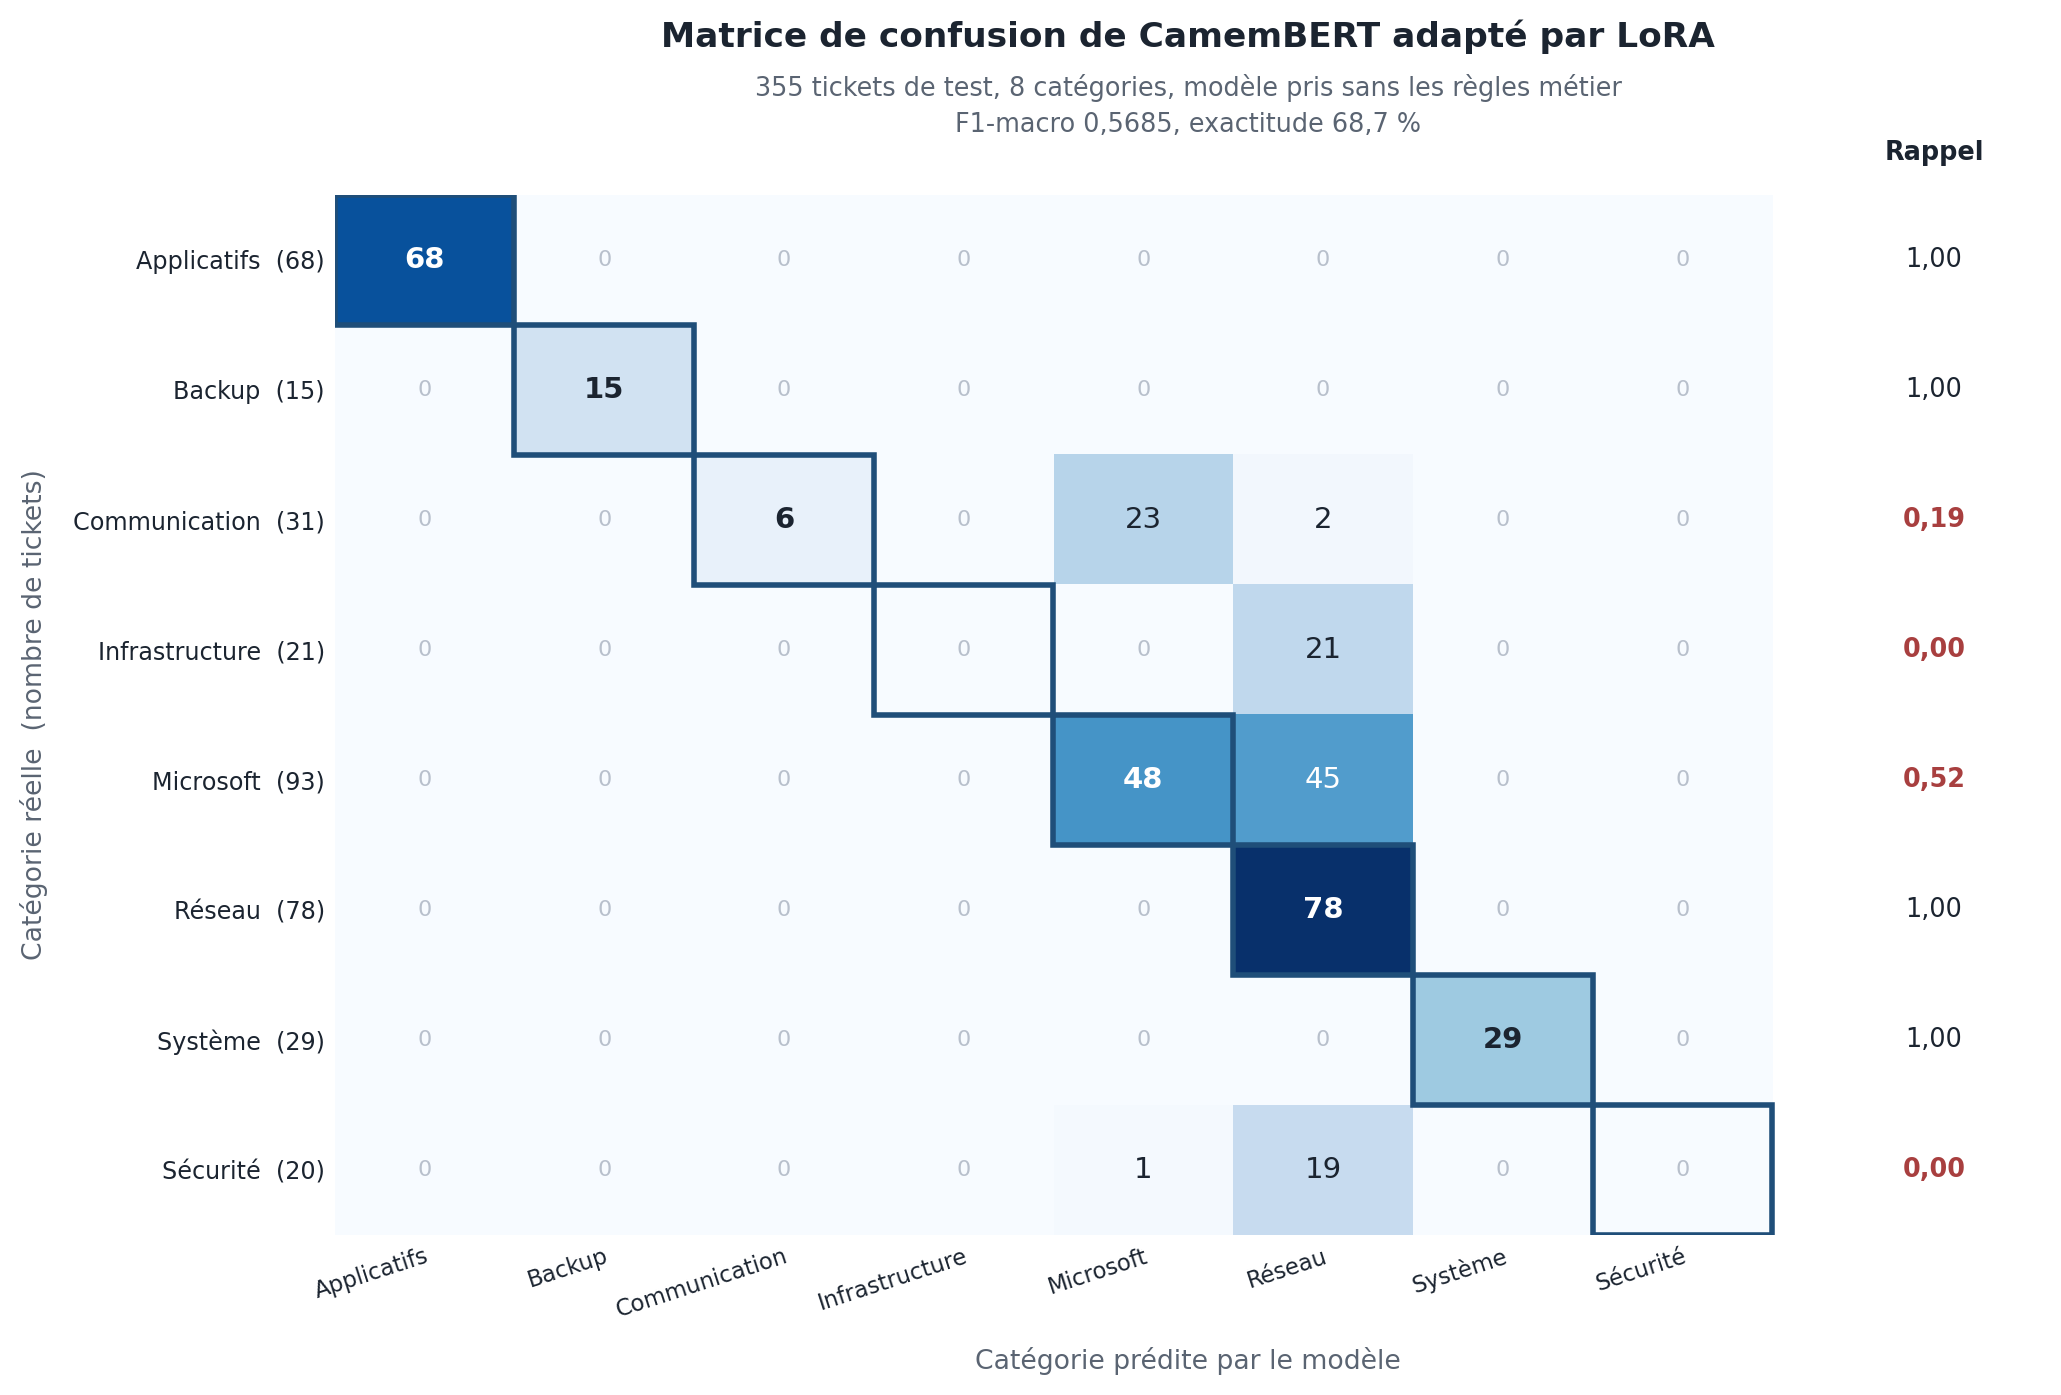
\includegraphics[width=0.92\textwidth]{ch04_confusion_camembert.png}
\caption{Matrice de confusion de CamemBERT adapté par LoRA}
\label{fig:camconf}
\end{figure}

Quatre catégories sont parfaitement traitées : \emph{Applicatifs}, \emph{Backup}, \emph{Réseau} et
\emph{Système}. \emph{Backup} est la surprise : la baseline y échouait totalement et les règles ne
la rattrapaient pas davantage.

Les erreurs se concentrent sur un point unique : \emph{Réseau} agit comme un attracteur. La totalité
des 21 tickets \emph{Infrastructure} y est versée, ainsi que 19 des 20 tickets \emph{Sécurité} et 45
des 93 tickets \emph{Microsoft}. Quand le modèle rencontre un scénario dont il n'a pas
l'équivalent, il le rattache à la catégorie dont il a vu la plus grande variété de formulations à
l'entraînement.

Le décompte sur \emph{Microsoft} se lit encore plus précisément. Les 93 tickets de cette catégorie
se répartissent en deux types, \og Microsoft Teams ne se lance plus \fg{} pour 48 d'entre eux et
\og OneDrive ne synchronise pas les fichiers \fg{} pour les 45 autres. Or le modèle classe
correctement 48 tickets et en verse 45 dans \emph{Réseau} : il traite le premier type sans aucune
erreur et le second sans aucune réussite. La décision se joue donc scénario par scénario : le sort
d'un ticket est celui de son type. Ce que le chapitre~3 avait établi sur les données se vérifie ici
sur les prédictions.

Préfixer chaque ticket de son type de demande et de sa priorité simplifiés, variables construites
au chapitre~3, fait passer le F1-macro de 0,5325 à 0,5685, soit un gain de 0,036. Ce préfixe donne
au modèle un signal que le texte libre ne porte pas toujours.

\section{Comparaison et analyse}

\subsection{Tableau d'ensemble}

La figure~\ref{fig:bench4} rassemble les sept approches sous le protocole unique de la
section~\ref{sec:protocole}.

\begin{figure}[!htbp]
\centering
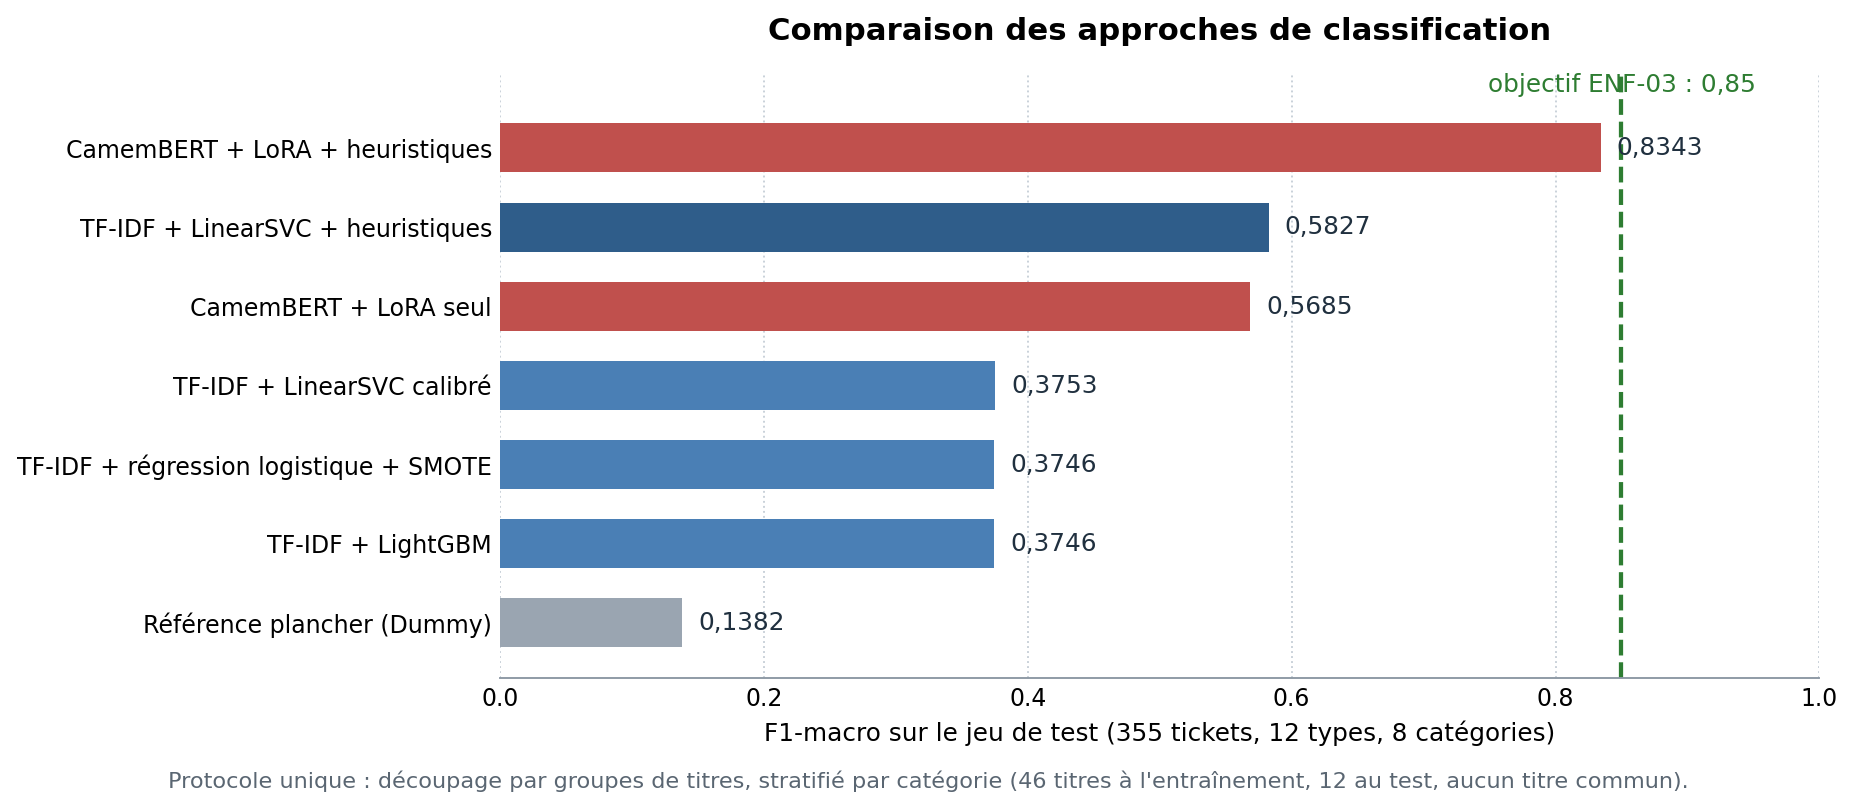
\includegraphics[width=\textwidth]{ch04_benchmark.png}
\caption{F1-macro des approches comparées, jeu de test de 355 tickets}
\label{fig:bench4}
\end{figure}

Quatre paliers se lisent sur ce graphique. Le hasard occupe le premier à 0,138. Les modèles
purement lexicaux forment le deuxième autour de 0,375, quelle que soit leur famille. Le troisième,
autour de 0,58, réunit l'approche par règles et le transformer seul. Le quatrième n'est occupé que
par leur combinaison, à 0,8343.

\subsection{La combinaison qui manquait}
\label{sec:combinaison}

La comparaison telle qu'elle vient d'être conduite oppose une chaîne lexicale complétée par des
règles à un transformer qui n'en reçoit aucune. Les deux systèmes ne sont donc pas dans la même
configuration, et l'écart mesuré entre eux ne dit rien de leurs mérites respectifs.

Les règles ne dépendent pourtant d'aucun modèle. Elles lisent le texte brut du ticket et reçoivent
une catégorie prédite accompagnée d'un score de confiance, sans se soucier de leur provenance. Rien
n'empêchait donc de les appliquer aux sorties de CamemBERT. Le tableau~\ref{tab:croise} donne les
quatre combinaisons.

\begin{table}[!htbp]
\centering
\styletableau
\caption{Les deux modèles, avec et sans les règles métier}
\label{tab:croise}
\begin{tabular}{|Bp{4.0cm}|Cp{2.8cm}|Cp{2.8cm}|Cp{2.6cm}|}
\hline
\rowcolor{enteteTab}
& \textbf{TF-IDF} & \textbf{CamemBERT} & \textbf{Écart} \\
\hline
Sans les règles & 0,3753 & 0,5685 & +0,1932 \\
\hline
Avec les règles & 0,5827 & \textbf{0,8343} & +0,2516 \\
\hline
Apport des règles & +0,2074 & +0,2658 & \\
\hline
\end{tabular}
\end{table}

Le tableau se lit dans les deux sens et donne deux résultats.

Dans les deux configurations, CamemBERT devance la chaîne lexicale, de 0,19 sans les règles et de
0,25 avec. L'hypothèse H1 du cahier des charges, selon laquelle un transformer francophone adapté
surpasse la baseline, est donc vérifiée. La lecture inverse, celle d'une égalité entre les deux
approches, provenait uniquement de la comparaison asymétrique.

Les règles profitent davantage au transformer qu'à la chaîne lexicale, +0,266 contre +0,207. Les
deux composants ne corrigent pas les mêmes erreurs. CamemBERT traite seul \emph{Backup} et
\emph{Système} à 1,00, là où la chaîne lexicale les abandonne ; les règles récupèrent
\emph{Infrastructure} et \emph{Sécurité}, que les deux modèles laissent à zéro. Leur combinaison
additionne deux couvertures complémentaires plutôt que de renforcer la même.

\subsection{Audit des règles métier}
\label{sec:audit}

Une vérification conduite en fin de sprint a révisé ces chiffres à la baisse, et la démarche mérite
d'être rapportée.

Les règles avaient été enrichies au fil des expériences. En reprenant leur historique, nous avons
constaté qu'un commentaire du code justifiait l'ajout d'un mot-clé par un titre appartenant au jeu
de test. Nous avons alors confronté chaque mot-clé au jeu d'entraînement. Quatre d'entre eux, réunis
au tableau~\ref{tab:audit}, n'y figuraient dans aucun ticket et ne se déclenchaient que sur des
tickets de test.

\begin{table}[!htbp]
\centering
\styletableau
\caption{Mots-clés retirés à l'issue de l'audit}
\label{tab:audit}
\begin{tabular}{|Bp{4.0cm}|Lp{3.4cm}|Cp{2.6cm}|Cp{2.6cm}|}
\hline
\rowcolor{enteteTab}
\textbf{Mot-clé} & \textbf{Catégorie forcée} & \textbf{Tickets d'entraînement} &
\textbf{Tickets de test} \\
\hline
\texttt{onedrive} & Microsoft & 0 & 45 \\
\hline
\texttt{san} & Infrastructure & 0 & 21 \\
\hline
\texttt{ids} & Sécurité & 0 & 12 \\
\hline
\texttt{acces non autorisé} & Sécurité & 0 & redondant \\
\hline
\end{tabular}
\end{table}

Un mot-clé introduit après avoir observé une erreur sur le jeu de test ajuste le système aux
données qui servent à le juger. Le score cesse alors de mesurer la généralisation et mesure la
mémorisation. Nous avons donc retiré ces quatre termes et remesuré l'ensemble des configurations.

L'effet est considérable. Le F1-macro de CamemBERT accompagné des règles passe de 0,9499 à 0,8343,
et celui de la chaîne lexicale de 0,7513 à 0,5827. La part non généralisable atteignait donc 0,116
d'un côté et 0,169 de l'autre. Tous les chiffres de ce chapitre sont ceux mesurés après retrait.

Ces quatre termes désignent pourtant des technologies dont la catégorie ne prête pas à discussion :
OneDrive est un produit Microsoft, un IDS un équipement de détection d'intrusion, un SAN une baie
de stockage. Le défaut ne tient pas à leur contenu mais au moment de leur introduction. Ils
pourraient être réintroduits si le service support les validait par écrit comme référentiel métier,
établi sans consultation des résultats de test. Cette validation n'a pas été obtenue dans le temps
du projet.

La règle de conduite retenue pour la suite figure désormais en tête du module de règles : un
mot-clé n'y est admis que s'il est attesté dans le jeu d'entraînement, ou s'il reste sans effet sur
le jeu de test.

\subsection{Ce qui sépare encore de l'objectif}
\label{sec:pourquoi}

Il manque 0,016 de F1-macro pour atteindre l'exigence ENF-03. Le détail par catégorie situe
précisément ce qui manque.

Six catégories sur huit dépassent 0,74 et quatre atteignent 1,00. La plus faible est
\emph{Microsoft}, à 0,4463, dont les 93 tickets de test se répartissent en deux scénarios : le
modèle traite le premier sans erreur et manque le second, faute du terme discriminant que l'audit a
écarté. Sa précision reste élevée, 0,96, mais son rappel tombe à 0,29.

Comme le F1-macro accorde un huitième du total à chaque catégorie, il suffirait que
\emph{Microsoft} passe de 0,4463 à 0,5719 pour franchir la barre des 0,85. Aucune autre catégorie
n'aurait besoin de bouger.

La limite de fond reste celle qu'a posée le chapitre~3. Le corpus contient 1\,800 tickets pour
58 scénarios distincts, dont 46 servent à l'entraînement. Ces 46 situations, répétées une trentaine
de fois chacune, sont tout ce dont dispose un modèle de langue conçu pour vivre de la diversité.
Ce qu'il faut ajouter au corpus se compte en scénarios, pas en tickets : multiplier les instances
d'un scénario déjà présent revient à recopier ce que le modèle sait déjà. Le chapitre~7 revient sur
ce point à propos de la boucle d'amélioration continue, qui vise précisément à faire entrer de
nouveaux scénarios au fil de l'exploitation.

\subsection{Le modèle retenu pour la production}
\label{sec:production}

Le système servi est le LinearSVC calibré accompagné des règles métier. Ce choix a été arrêté au
moment où les deux approches paraissaient équivalentes, et il reposait sur trois arguments
étrangers à la performance.

L'inférence de CamemBERT exige de charger 110 millions de paramètres, là où la chaîne TF-IDF tient
dans un fichier de 326\,ko. L'exigence ENF-01 fixe la latence de prédiction à 300\,ms au
quatre-vingt-quinzième centile, et le chapitre~7 montrera qu'elle n'est déjà pas tenue avec la
chaîne légère : lui substituer un transformer aggraverait un écart existant. Enfin, une décision
produite par des règles nommées s'explique au consultant, et le chapitre~1 a placé ce système en
position d'assistant.

La comparaison à configuration égale déplace cet arbitrage. Un écart de 0,25 de F1-macro ne se
compense pas par la légèreté d'un artefact, d'autant que les deux systèmes partagent la même couche
de règles et donc la même explicabilité sur les décisions qu'elle produit. La mise en service de
CamemBERT suppose de traiter d'abord la latence, par exemple en réservant le transformer aux
tickets dont la chaîne lexicale n'est pas sûre. Nous la portons aux perspectives plutôt que de
l'engager en fin de projet.

L'adaptateur reste versionné dans le dépôt et la porte de promotion décrite au chapitre~7 accepte
un modèle de cette nature, à condition qu'il soit évalué sur le même jeu de test gelé.

Nous conservons l'adaptateur CamemBERT dans le dépôt. Il documente la comparaison et resterait
mobilisable si le corpus gagnait en diversité.

Le pipeline réentraîne le modèle de production, donc sous le découpage non stratifié.
Ses chiffres, rapportés au tableau~\ref{tab:prod}, ne sont pas comparables à ceux qui précèdent.

\begin{table}[!htbp]
\centering
\styletableau
\caption{Modèle de production, mesuré sous le protocole du pipeline}
\label{tab:prod}
\begin{tabular}{|Bp{6.2cm}|Cp{2.6cm}|Lp{4.4cm}|}
\hline
\rowcolor{enteteTab}
\textbf{Indicateur} & \textbf{Valeur} & \textbf{Portée} \\
\hline
F1-macro, modèle seul & 0,2708 & 8 catégories \\
\hline
F1-macro avec les règles & 0,5829 & 8 catégories, dont 3 sans exemple \\
\hline
F1-macro sur les catégories évaluables & 0,6995 & 5 catégories ayant du support \\
\hline
Exactitude & 0,8202 & 356 tickets \\
\hline
Précision macro & 0,5868 & 5 catégories \\
\hline
Rappel macro & 0,6099 & 5 catégories \\
\hline
Part des tickets corrigés par une règle & 37,4\,\% & 356 tickets \\
\hline
\end{tabular}
\end{table}

Les trois catégories absentes du jeu de test expliquent seules l'écart entre 0,5829 et 0,6995 :
leur F1 vaut zéro parce qu'aucun ticket ne les représente, non parce que le modèle les manque. Nous
rapportons les deux valeurs ; la seconde sert de métrique de décision au mécanisme de promotion
décrit au chapitre~7. Aucune des deux n'est comparable au 0,5827 du protocole stratifié.

Le rappel sur \emph{Sécurité} tombe à zéro sous ce protocole, pour une exigence ENF-04 fixée à
0,70. Les trois scénarios de sécurité tirés au test relèvent tous de l'intrusion détectée, et le
terme qui les caractérisait a été écarté par l'audit. Le même système atteint un rappel de 0,40 sur
cette catégorie sous le protocole stratifié, où d'autres scénarios sont tirés. Cet écart de zéro à
0,40 pour un système inchangé illustre ce que le chapitre~3 annonçait : sur douze scénarios de
test, une mesure par catégorie se déplace par paliers entiers.

\subsection{Calibration de la confiance et routage}
\label{sec:calibration}

Le système renvoie un score de confiance destiné à décider quels tickets peuvent être routés
automatiquement et lesquels demandent une revue humaine. Encore faut-il que ce score ordonne
correctement la fiabilité. Le tableau~\ref{tab:calib} confronte les tranches de confiance à la
précision réellement observée dans chacune.

\begin{table}[!htbp]
\centering
\styletableau
\caption{Précision observée par tranche de confiance, protocole des expériences}
\label{tab:calib}
\begin{tabular}{|Bp{3.0cm}|Cp{2.4cm}|Cp{2.2cm}|Cp{2.6cm}|}
\hline
\rowcolor{enteteTab}
\textbf{Tranche} & \textbf{Tickets} & \textbf{Part} & \textbf{Précision} \\
\hline
Sous 40\,\% & 42 & 11,8\,\% & 0,0\,\% \\
\hline
40 à 60\,\% & 121 & 34,1\,\% & 33,9\,\% \\
\hline
60 à 80\,\% & 110 & 31,0\,\% & 89,1\,\% \\
\hline
Au-dessus de 80\,\% & 82 & 23,1\,\% & 81,7\,\% \\
\hline
\end{tabular}
\end{table}

Le score sépare correctement les deux extrémités : sous 40\,\%, aucune prédiction n'est juste ;
au-delà de 60\,\%, plus de quatre sur cinq le sont. La distribution de la
figure~\ref{fig:confiance} montre cette séparation sur le modèle CamemBERT.

\begin{figure}[!htbp]
\centering
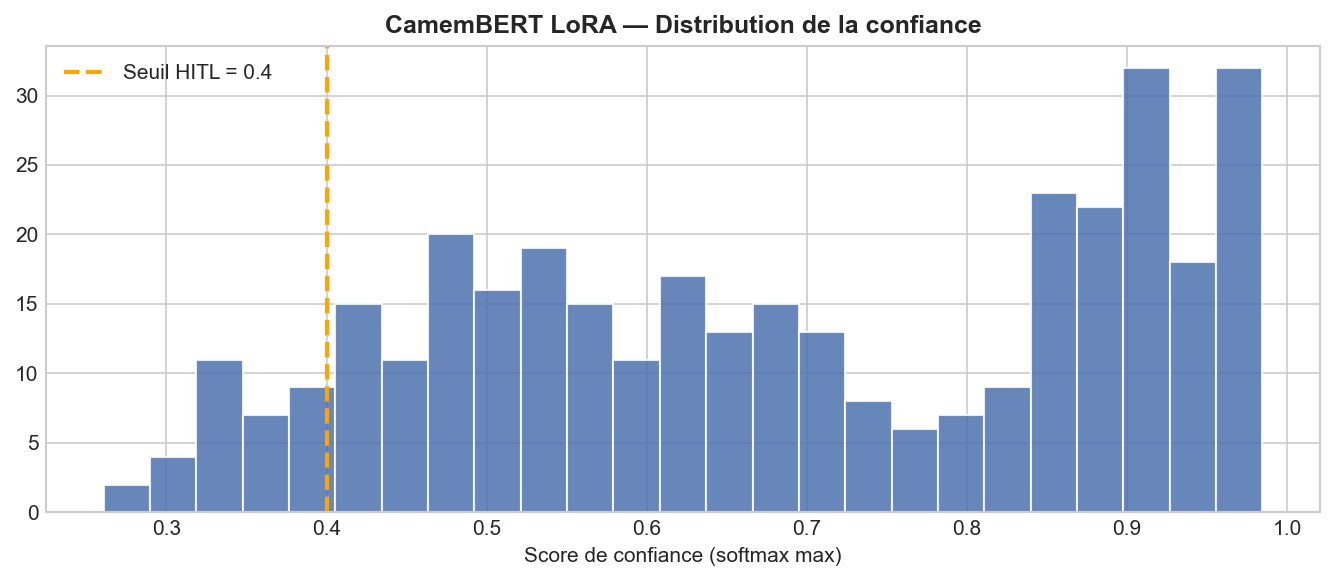
\includegraphics[width=0.92\textwidth]{ch04_confiance.png}
\caption{Distribution des scores de confiance et seuil de routage}
\label{fig:confiance}
\end{figure}

Une anomalie subsiste néanmoins. La tranche 60 à 80\,\% est plus fiable, à 89,1\,\%, que la tranche
supérieure à 80\,\%, qui tombe à 81,7\,\%. Un score de confiance devrait être monotone : plus il est
élevé, plus la prédiction devrait être sûre. Il ne l'est pas ici. Le score renseigne donc sur
l'ordre de grandeur de la fiabilité, sans permettre de distinguer finement deux prédictions toutes
deux assurées. C'est la réserve portée à l'objectif~6.

Nous avions d'abord fixé le seuil de routage à 0,40, valeur qui envoie 88,2\,\% des tickets en
traitement automatique pour une précision de 65,8\,\%. Un tel réglage laisse passer un tiers
d'erreurs sans relecture, ce qui contredit le principe de maintien de la décision humaine posé en
introduction du mémoire. Nous l'avons relevé à 0,60 dans la configuration de production. Les
métadonnées du modèle annoncent pour ce nouveau seuil environ 70\,\% de routage automatique et
85\,\% de précision ; il s'agit d'une estimation, que le jeu de test n'a pas servi à vérifier.

\section{Bilan du sprint}

Le sprint livre un protocole d'évaluation explicite, sept approches comparées sous ce protocole, un
module de règles métier audité, un adaptateur CamemBERT entraîné sous contrainte matérielle, et le
modèle servi en production avec son seuil de routage.

L'exigence ENF-03 visait 0,85 et la meilleure combinaison atteint 0,8343 sous le protocole
stratifié. L'écart de 0,016 tient à une seule catégorie, \emph{Microsoft}, dont le terme
discriminant a été écarté faute de support à l'entraînement.

L'exigence ENF-04 visait un rappel d'au moins 0,70 sur \emph{Sécurité}, et elle n'est atteinte dans
aucune configuration. Le meilleur rappel mesuré est 0,60, obtenu par CamemBERT accompagné des
règles sur le protocole stratifié ; la chaîne lexicale plafonne à 0,40 sur le même jeu et à zéro
sous le protocole du pipeline. La précision, elle, vaut 1,00 dans les deux cas : chaque incident de
sécurité annoncé en est bien un, mais quatre sur dix échappent au système dans le meilleur des cas.
Nous reportons ces deux écarts au registre des risques du projet.

Le sprint livre aussi un résultat de méthode. L'audit des règles a retiré quatre mots-clés
introduits en observant le jeu de test et a fait baisser le meilleur score de 0,9499 à 0,8343. Un
projet qui ne mène pas cette vérification publie des chiffres qu'il croit sincères. Nous
considérons ce retrait comme un acquis du sprint au même titre que les modèles entraînés.

Le sprint établit enfin un diagnostic qui oriente la suite. Le plafond rencontré est celui des
46 scénarios distincts disponibles à l'entraînement. Deux conséquences en découlent pour le reste
du mémoire. Le chapitre~5 met la redondance du corpus à profit : un moteur de recherche par
similarité tire parti de ce qui embarrasse un classifieur. Le chapitre~7 construit le mécanisme qui
permettra au corpus de gagner des scénarios au fil de l'exploitation.

\section*{Conclusion}
\addcontentsline{toc}{section}{Conclusion}

Trois approches ont été éprouvées sous un protocole unique, qui couvre les huit catégories. La
vectorisation classique atteint 0,3753 et ignore la moitié du référentiel. Lui adjoindre les règles
métier porte le résultat à 0,5827 : les catégories abandonnées reviennent. CamemBERT adapté par
LoRA atteint 0,5685 sans aucune règle.

Le résultat décisif vient de leur combinaison, que la comparaison initiale n'avait pas éprouvée.
Les règles ne dépendent d'aucun modèle : elles lisent le texte brut et corrigent une catégorie
prédite, quelle qu'en soit l'origine. Appliquées aux sorties du transformer, elles portent le
F1-macro à \textbf{0,8343}, à 0,016 de l'objectif. CamemBERT devance la chaîne lexicale dans les
deux configurations, de 0,19 sans les règles et de 0,25 avec, ce qui vérifie l'hypothèse H1 du
cahier des charges.

Ce chiffre est celui qui subsiste après l'audit des règles. Quatre mots-clés absents du jeu
d'entraînement et actifs sur le seul jeu de test ont été retirés, ce qui a ramené le meilleur score
de 0,9499 à 0,8343. La différence mesurait ce que le système avait mémorisé plutôt qu'appris.

Le modèle mis en service reste la chaîne TF-IDF complétée par les règles, choisie pour sa latence
et sa légèreté à un moment où les deux approches paraissaient équivalentes. L'écart désormais
mesuré invite à rouvrir cet arbitrage, ce que la conclusion générale porte aux perspectives. Le
score de confiance sépare utilement les prédictions fiables des autres sans être strictement
monotone, ce qui justifie de conserver la revue humaine sur les cas peu assurés.

Le chapitre~5 construit le second volet de la solution : un moteur de recherche qui retrouve dans
l'historique les résolutions comparables, et pour lequel la redondance du corpus devient un atout.

        \clearpage

        \chapter{Système RAG et assistance intelligente}

\section*{Introduction}
\addcontentsline{toc}{section}{Introduction}

Le classifieur du chapitre précédent affecte une catégorie à chaque ticket. Savoir qu'une demande
relève de la catégorie \emph{Microsoft} oriente son affectation sans dire comment la traiter. Ce
chapitre construit le second volet de la solution : un moteur qui retrouve dans l'historique les
tickets comparables et présente leur résolution à l'administrateur. La redondance du corpus, qui a
bridé le classifieur, devient ici un atout, puisque cinquante-huit scénarios réinstanciés rendent
probable qu'un nouveau ticket ressemble à un ticket déjà résolu.

Trois moteurs ont été construits et comparés sous un protocole unique, recherche lexicale,
recherche sémantique et leur combinaison, complétés par un modèle de langage exécuté sur
l'infrastructure du service. Deux résultats et deux limites sont annoncés d'emblée.

\begin{puces}
  \item Le moteur hybride, celui qui est servi, obtient la meilleure précision à trois passages,
        0,3542 contre 0,2917 pour le sémantique seul.
  \item Sa similarité moyenne, 0,3551, n'atteint jamais le seuil de pertinence de 0,50 : aucune des
        quatre-vingts requêtes d'évaluation n'a été servie autrement que par le mécanisme de repli
        (section~\ref{sec:seuil5}).
  \item Aucun jeu d'évaluation annoté n'existe pour la recherche, si bien que les mesures reposent
        sur un protocole indicatif (section~\ref{sec:eval5}).
  \item Le découpage anti-fuite place les scénarios du jeu de test hors de la base : aucune requête
        d'évaluation n'admet de bonne réponse, et les valeurs constituent un plancher
        (section~\ref{sec:antifuite5}).
\end{puces}

\section{Présentation du système RAG}

Le principe de la génération augmentée par récupération, introduit par Lewis et
ses coauteurs~\cite{lewis2020} et depuis largement décliné~\cite{gao2023}, a été exposé au
chapitre~2. Sa déclinaison ici tient en peu de mots : une demande entrante est comparée aux résolutions déjà consignées, les
plus proches sont retenues, un modèle de langage les reformule avant affichage. Le système ne
produit aucune connaissance nouvelle, il retrouve et met en forme ce que le service sait déjà.

La figure~\ref{fig:chaine5} donne la chaîne servie sur deux niveaux. En haut le parcours de
recommandation, du ticket entrant à la réponse reformulée ; en bas le parcours d'alimentation, par
lequel une solution validée par un administrateur revient enrichir la base.

\begin{figure}[!htbp]
\centering
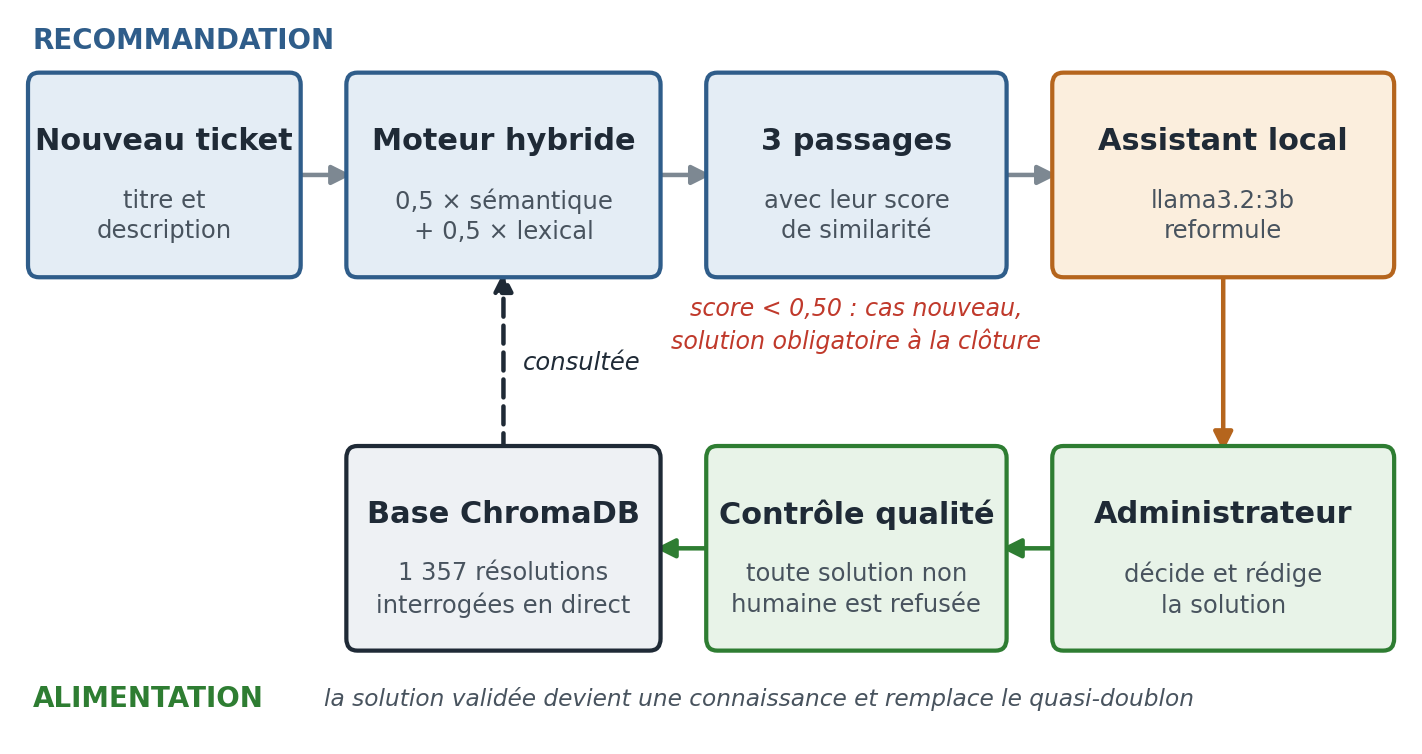
\includegraphics[width=\textwidth]{ch05_chaine_rag.png}
\caption{Chaîne servie du système RAG}
\label{fig:chaine5}
\end{figure}

\FloatBarrier

\section{Construction de la base de connaissances}

\subsection{Composition de la base}

La base est produite par le module de découpage du corpus, au même moment que les jeux
d'entraînement et de test. Elle retient tout ticket du jeu d'entraînement dont le champ
\emph{Résolution\,/\,Motif} est renseigné, soit \textbf{1\,357 tickets} sur les huit catégories du
référentiel, sans restriction au statut \emph{Résolu}.

\begin{table}[!htbp]
\centering
\styletableau
\caption{Composition de la base de connaissances par statut de ticket}
\label{tab:kb5}
\begin{tabular}{|Lp{4.6cm}|Cp{2.4cm}|Lp{6.4cm}|}
\hline
\rowcolor{enteteTab}
\textbf{Statut du ticket} & \textbf{Effectif} & \textbf{Ce que le champ contient} \\
\hline
Rejeté & 363 & Le motif du refus, qui vaut réponse pour une demande semblable \\
\hline
Résolu & 358 & La procédure appliquée \\
\hline
Problème & 237 & Le diagnostic posé, la cause identifiée \\
\hline
Prise en charge & 236 & L'action engagée et son état d'avancement \\
\hline
En attente & 163 & L'élément manquant qui bloque le traitement \\
\hline
\rowcolor{enteteTab}
\textbf{Total} & \textbf{1\,357} & \\
\hline
\end{tabular}
\end{table}

Un rejet documenté répond à une question réelle du demandeur, et l'écarter priverait la base d'un
quart de sa matière. La contrepartie est admise : un ticket \emph{En attente} décrit un blocage
plutôt qu'une solution. Nous avons retenu la couverture large parce que l'administrateur reste seul
décideur.

Ces documents sont conservés dans ChromaDB, que le service applicatif interroge directement, et
indexés selon les deux représentations de la section suivante. La base n'est pas figée : la
section~\ref{sec:boucle5} montre comment une solution validée en exploitation vient s'y ajouter.

\subsection{Format des résolutions}

Les textes retenus sont courts, de longueur médiane \textbf{12 mots} et d'étendue 7 à 16 mots.

\begin{quote}
\og Vérifier les entrées DNS, vider le cache DNS client, forcer l'enregistrement du serveur. \fg{}
\end{quote}

Une résolution de douze mots énumère des gestes sans les expliquer. Elle vaut comme repère pour un
technicien du domaine, non comme procédure autonome. Cette brièveté limite ce qu'un modèle de
langage peut en tirer, puisqu'il n'a rien à résumer, et explique que l'assistant de la
section~\ref{sec:llm5} soit conçu pour reformuler. Le moteur épargne une recherche manuelle dans
plusieurs milliers de lignes, il ne remplace pas l'expertise de l'administrateur.

\subsection{Volume indexé et diversité réelle des réponses}
\label{sec:diversite5}

Le décompte de 1\,357 tickets décrit un volume, non une richesse. Les tickets indexés portent
\textbf{46 résolutions distinctes} pour 46 titres distincts, dans une correspondance exacte : à
chaque scénario du corpus d'entraînement répond une résolution et une seule, réinstanciée en
médiane 31 fois, de 4 à 49 fois selon les cas.

\begin{table}[!htbp]
\centering
\styletableau
\caption{Nombre de résolutions distinctes par catégorie dans la base de connaissances}
\label{tab:diversite5}
\begin{tabular}{|Bp{3.4cm}|Cp{3.0cm}|Bp{3.4cm}|Cp{3.0cm}|}
\hline
\rowcolor{enteteTab}
\textbf{Catégorie} & \textbf{Réponses} & \textbf{Catégorie} & \textbf{Réponses} \\
\hline
Applicatifs & 8 & Microsoft & 6 \\
\hline
Réseau & 8 & Communication & 5 \\
\hline
Backup & 6 & Système & 5 \\
\hline
Infrastructure & 4 & Sécurité & 4 \\
\hline
\end{tabular}
\end{table}

La conséquence est double. Un incident récurrent trouve la réponse exacte que le service a déjà
appliquée, usage précisément visé ; un incident inédit ne trouve rien, la base ne couvrant que
quarante-six situations. Quatre réponses pour toute la catégorie \emph{Sécurité} laissent peu de
marge à la variété des incidents que ce mot recouvre.

\subsection{Le coût de la contrainte anti-fuite}
\label{sec:antifuite5}

Aucun ticket du jeu de test ne figure dans la base. Sans cette restriction, une requête
d'évaluation s'y retrouverait elle-même avec une similarité proche de~1, et toute mesure de qualité
deviendrait sans objet.

Son coût est plus lourd qu'il n'y paraît. Le découpage étant groupé par titre, les 58 scénarios du
corpus se répartissent en deux ensembles \textbf{disjoints}, 46 pour la base et 12 pour le jeu de
test. Les 356 tickets de ce jeu appartiennent donc tous à des scénarios dont \textbf{aucune
résolution ne figure dans la base} : aucune requête d'évaluation n'admet de bonne réponse, et le
moteur ne peut au mieux que proposer le voisin le plus plausible venu d'un autre scénario. Deux
règles de lecture en découlent.

\begin{puces}
  \item Les valeurs de la section~\ref{sec:resultats5} constituent un \textbf{plancher}, non une
        estimation du service rendu en exploitation, où un incident récurrent retrouve les
        instances antérieures de son propre scénario.
  \item Les scores de similarité mesurés sont bas par construction, ce dont la
        section~\ref{sec:seuil5} tire les conséquences.
\end{puces}

\FloatBarrier

\section{Mise en œuvre de la recherche}

\subsection{Recherche lexicale}

Le premier moteur applique la représentation vectorielle du chapitre~4, pondération TF-IDF sur cinq
mille descripteurs en unigrammes et bigrammes, avec classement par similarité cosinus dans l'espace
des documents indexés.

Ce moteur trouve un ticket lorsque la demande et la résolution partagent des mots, ce qui le rend
précis sur les formulations exactes et aveugle au reste. La limite n'est pas théorique dans un
corpus rédigé par des utilisateurs : une même panne de messagerie se dit \og je ne reçois plus mes
mails \fg{}, \og la synchronisation échoue \fg{} ou \og Outlook ne se connecte plus \fg{}, sans
qu'aucun mot commun ne subsiste.

\subsection{Recherche sémantique}

Le second moteur encode chaque ticket par un modèle de plongements de phrases,
\texttt{paraphrase-multilingual-mpnet-base-v2}, qui produit un vecteur de 768 dimensions. Ce modèle
traite le français sans traduction intermédiaire, a été entraîné à rapprocher des paraphrases et
s'exécute sans accélération graphique.

L'index est construit avec FAISS, en produit scalaire sur vecteurs normalisés. Cette normalisation
rend le produit scalaire égal au cosinus, donc la similarité bornée entre $-1$ et~$1$ et comparable
d'une requête à l'autre. Un index global est complété par un index par catégorie, ce qui permet de
restreindre la recherche lorsque la catégorie prédite est jugée fiable.

\subsection{Recherche hybride}

Le troisième moteur interroge les deux précédents et fusionne leurs scores. Nous retenons une
combinaison linéaire des scores plutôt qu'une fusion par les rangs~\cite{cormack2009}, afin de
conserver une échelle de similarité comparable à celle du seuil de pertinence :

\[
\text{score}_{\text{hybride}} = \alpha \cdot \text{score}_{\text{sémantique}}
+ (1 - \alpha) \cdot \text{score}_{\text{lexical}}
\]

Le paramètre $\alpha$ vaut 0,5 dans la configuration servie. Chaque sous-moteur remonte quinze
candidats sans filtrage, la fusion s'applique ensuite, le filtrage par seuil intervient en dernier,
ordre qui évite qu'un ticket écarté trop tôt soit perdu pour la fusion. L'intention est de réunir
la tolérance à la reformulation du sémantique et la précision du lexical sur les tickets répétés à
l'identique ; la section~\ref{sec:seuil5} montre l'effet secondaire que cette fusion produit.

\subsection{Comparaison des approches}

Ce qui sépare les trois moteurs tient moins à leur qualité qu'à ce que chacun sait voir.

\begin{table}[!htbp]
\centering
\styletableau
\caption{Ce que chaque moteur retrouve, et ce qui lui échappe}
\label{tab:comparaison5}
\begin{tabular}{|Bp{2.4cm}|Lp{5.6cm}|Lp{5.4cm}|}
\hline
\rowcolor{enteteTab}
\textbf{Moteur} & \textbf{Ce qu'il retrouve} & \textbf{Ce qui lui échappe} \\
\hline
Lexical & Les tickets qui emploient les mêmes mots que la demande & Un incident décrit avec un
autre vocabulaire \\
\hline
Sémantique & Les tickets qui décrivent le même incident, quels que soient les mots & Les
formulations exactes que le lexical classe en tête \\
\hline
Hybride & Les deux, par fusion à poids égal & Rien de plus, mais son échelle de score n'est plus
celle sur laquelle le seuil a été calibré \\
\hline
\end{tabular}
\end{table}

\FloatBarrier

\section{Évaluation du RAG}
\label{sec:eval5}

\subsection{Protocole et approximation de la pertinence}

La campagne interroge les trois moteurs avec quatre-vingts requêtes du jeu de test, en demandant
trois passages, et les sollicite exactement comme le fait l'application, mécanisme de repli
compris. Quatre indicateurs sont calculés.

\begin{puces}
  \item \textbf{Précision à trois passages} : proportion de passages pertinents parmi les trois
        retournés.
  \item \textbf{Rang réciproque moyen} : récompense un premier passage pertinent placé tôt.
  \item \textbf{Gain cumulé actualisé normalisé} : pondère chaque passage pertinent par sa position
        et rapporte le résultat au classement idéal.
  \item \textbf{Similarité moyenne} : valeur brute rendue par le moteur, comparée au seuil de
        pertinence.
\end{puces}

Décider si un passage est pertinent suppose de savoir ce qui l'est, information qui n'existe pas :
aucun jeu de référence annoté n'a été constitué. Le protocole considère comme pertinent tout
passage de la même catégorie que la requête. La règle est grossière, deux tickets \emph{Réseau}
pouvant décrire des incidents sans rapport.

Une raison plus contraignante que l'absence d'annotation impose cette approximation. Les scénarios
du jeu de test et ceux de la base sont disjoints (section~\ref{sec:antifuite5}), si bien qu'une
définition stricte donnerait \textbf{zéro} pour les trois moteurs, la bonne réponse étant absente
de l'index par construction. Le fichier de résultats porte cet avertissement : les valeurs servent
à \textbf{comparer les trois moteurs entre eux}, elles ne mesurent pas la pertinence perçue par un
administrateur. Le rappel à trois passages n'est pas publié pour la même raison, l'ensemble des
passages pertinents étant la catégorie entière, soit plusieurs centaines de tickets.

\subsection{Dimensions non couvertes par la campagne}

Deux dimensions échappent entièrement à la campagne, et le fichier de résultats les énumère.

\begin{puces}
  \item La \textbf{fidélité de la génération}. Le chemin de classification n'appelle aucun modèle
        de langage, et la reformulation destinée à l'administrateur constitue un appel séparé et
        facultatif, qui supposerait un protocole distinct.
  \item L'\textbf{utilité perçue}. Elle demanderait un retour explicite de l'administrateur sur
        chaque recommandation, que l'interface ne collecte pas.
\end{puces}

La commande d'évaluation produit sur option le gabarit d'annotation, soit quatre-vingts requêtes et
leurs dix meilleurs candidats. Le travail restant se compte en une demi-journée d'annotation par un
administrateur du service, et la conclusion générale porte cette lacune aux perspectives.

\FloatBarrier

\subsection{Résultats mesurés}
\label{sec:resultats5}

\begin{figure}[!htbp]
\centering
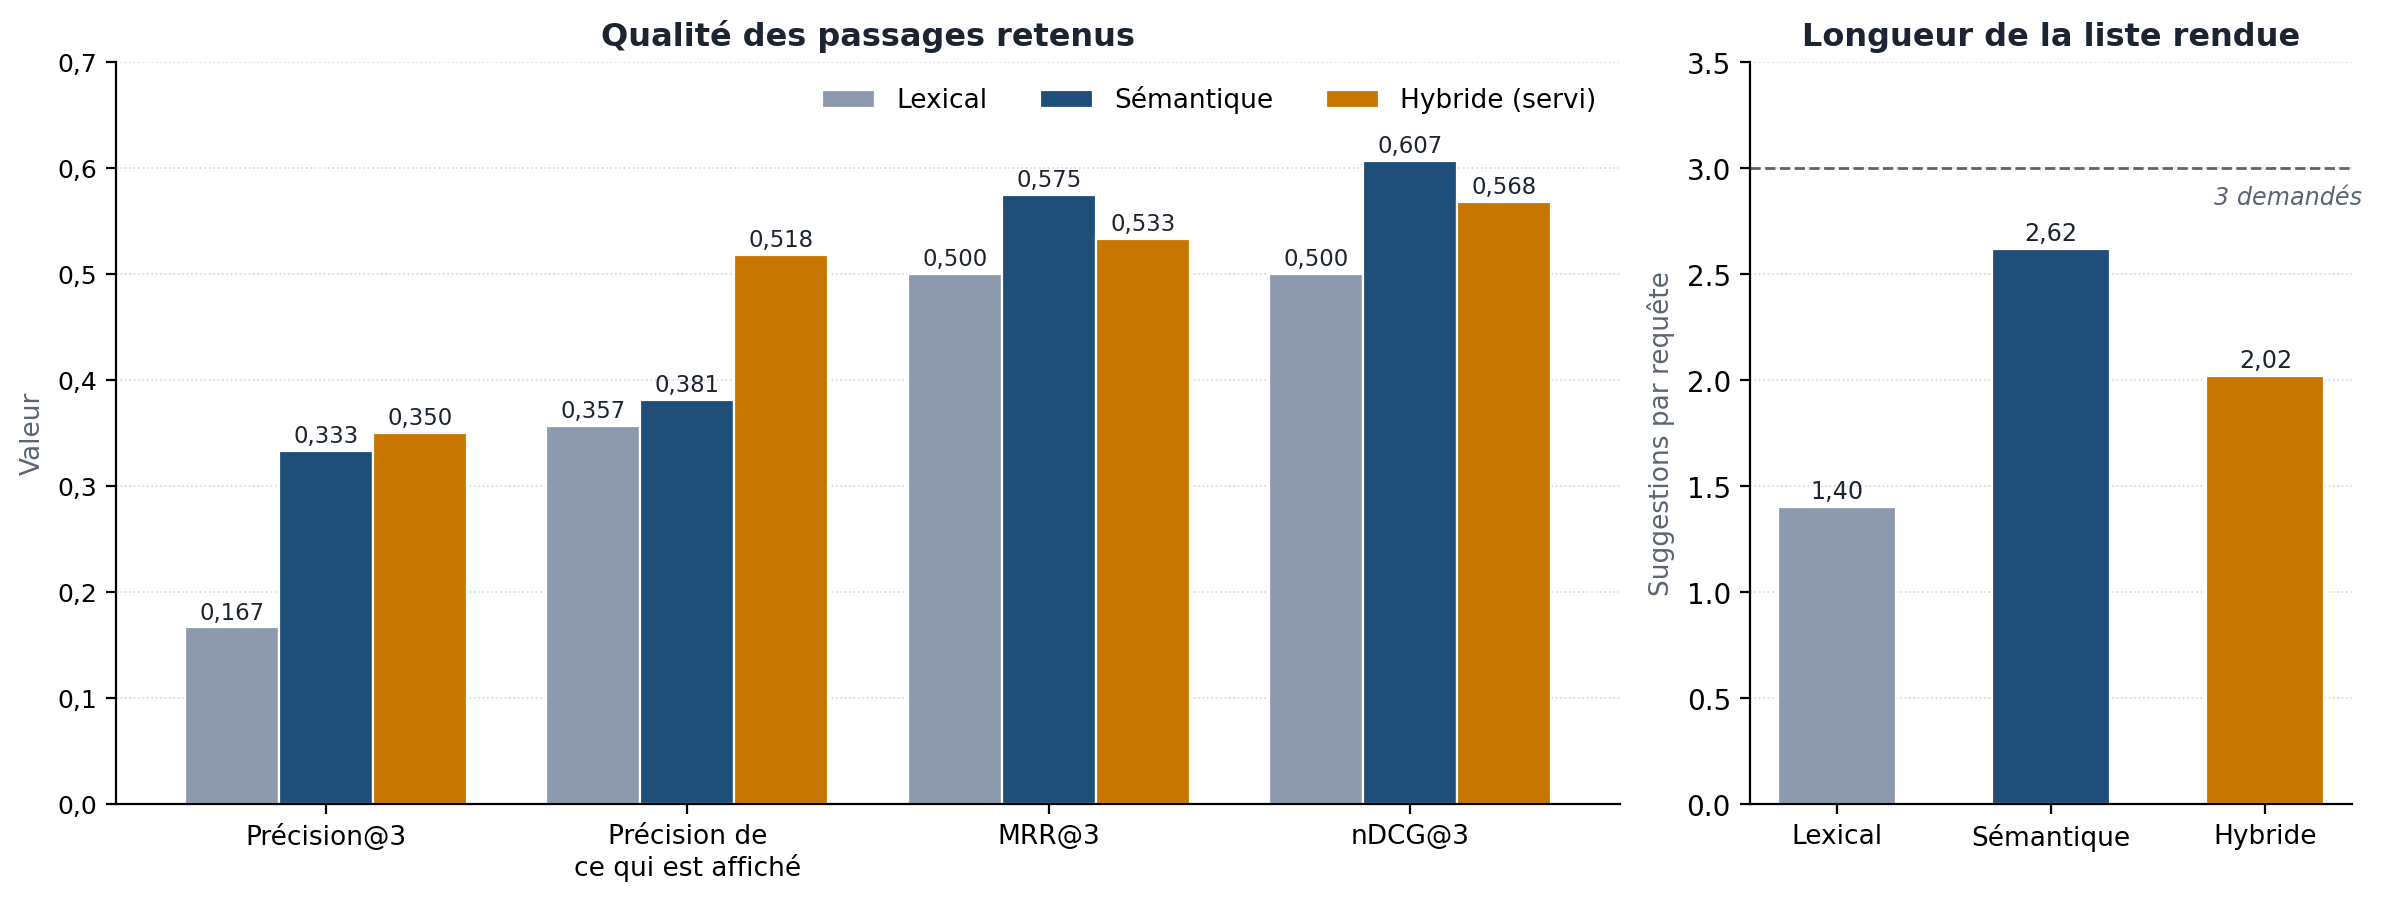
\includegraphics[width=\textwidth]{ch05_moteurs.png}
\caption{Comparaison des trois moteurs de recherche, 80 requêtes du jeu de test, trois passages
demandés}
\label{fig:moteurs5}
\end{figure}

\begin{table}[!htbp]
\centering
\styletableau
\caption{Comparaison des trois moteurs de recherche sous le protocole d'approximation}
\label{tab:moteurs5}
\begin{tabular}{|Bp{3.0cm}|Cp{2.0cm}|Cp{1.8cm}|Cp{1.8cm}|Cp{2.2cm}|Cp{1.8cm}|}
\hline
\rowcolor{enteteTab}
\textbf{Moteur} & \textbf{Précision @3} & \textbf{MRR @3} & \textbf{nDCG @3} &
\textbf{Similarité moyenne} & \textbf{Taux de repli} \\
\hline
Lexical & 0,1542 & 0,4354 & 0,4391 & 0,2117 & 1,000 \\
\hline
Sémantique & 0,2917 & \textbf{0,5813} & \textbf{0,5960} & \textbf{0,6099} & 0,0125 \\
\hline
Hybride (servi) & \textbf{0,3542} & 0,5375 & 0,5754 & 0,3551 & 1,000 \\
\hline
\end{tabular}
\end{table}

Le moteur sémantique domine le lexical sur les quatre indicateurs, l'écart le plus net portant sur
la précision, de 0,1542 à 0,2917, et sur la similarité moyenne, de 0,2117 à 0,6099. Dans un corpus
rédigé en langage libre, la proximité de sens retrouve des cas que le partage de vocabulaire
manque.

Le moteur hybride obtient la meilleure précision mesurée, 0,3542, quand ses indicateurs de
classement restent derrière le sémantique, 0,5375 contre 0,5813 pour le rang réciproque et 0,5754
contre 0,5960 pour le gain cumulé. La précision compte les passages pertinents sans considérer leur
ordre, tandis que les deux autres récompensent le fait de placer le bon passage en tête : la fusion
fait entrer dans le trio de tête des passages que le sémantique écartait, en ordonnant l'ensemble
un peu moins bien. Pour un usage où l'administrateur lit les trois propositions, la précision est
l'indicateur qui compte, ce qui justifie le choix du moteur hybride.

\subsection{Le seuil que le moteur servi n'atteint jamais}
\label{sec:seuil5}

Le paramétrage fixe un seuil de pertinence à 0,50 et un seuil de repli à 0,20. Une requête dont
aucun passage n'atteint 0,50 n'est servie que par le repli, et la dernière colonne du
tableau~\ref{tab:moteurs5} compte ces requêtes : 0,0125 pour le sémantique, soit une requête sur
quatre-vingts, et \textbf{1,000} pour l'hybride.

Le mécanisme est arithmétique. Le score hybride est la moyenne du score sémantique, 0,6099, et du
score lexical, 0,2117, soit 0,3551, très en dessous de 0,50. Atteindre le seuil avec un score
lexical de l'ordre de 0,21 exigerait un score sémantique d'environ 0,79, valeur que le moteur
sémantique lui-même n'atteint pas en moyenne. Le seuil a donc été calibré sur l'échelle du moteur
sémantique puis conservé tel quel, alors que la fusion change l'échelle des scores en même temps
que le classement.

Un second facteur pèse sur ces valeurs sans se confondre avec le premier : les scores sont bas en
partie parce qu'aucune requête d'évaluation n'a sa réponse dans la base
(section~\ref{sec:antifuite5}). Le diagnostic d'échelle reste valable indépendamment, la moyenne
avec un score lexical borné vers 0,21 divisant par deux l'écart au seuil.

La conséquence sur l'application est directe. Le module de traitement des tickets utilise le même
seuil de 0,50 pour décider qu'un ticket constitue un \emph{cas nouveau}, pour lequel
l'administrateur doit rédiger la solution appliquée avant de clore : un score systématiquement
inférieur revient à traiter tout ticket comme un cas nouveau. L'effet garantit que la base est
alimentée à chaque clôture, ce qui est l'intention de la boucle décrite à la
section~\ref{sec:boucle5}, mais il l'obtient par accident de calibrage et prive le seuil de sa
fonction de discrimination. Deux corrections sont envisageables, que nous énonçons sans trancher
faute de trafic réel : relever $\alpha$ pour rapprocher l'échelle hybride de l'échelle sémantique,
ou fixer un seuil propre au moteur hybride.

\subsection{Une mesure ancienne à ne pas citer}

Les métadonnées du moteur sémantique rapportent une similarité moyenne de 0,9321 contre 0,7646 pour
la recherche lexicale. Un lecteur qui ouvre ces fichiers rencontrera ces nombres, que deux
précisions écartent de toute citation.

La quantité mesurée n'est pas celle du tableau~\ref{tab:moteurs5} : il s'agit de la similarité du
\emph{meilleur} passage, quand la campagne rapporte la similarité moyenne des \emph{trois} passages
retenus. Et cette mesure a été conduite sur un index de \textbf{476 documents}, à un stade
antérieur du projet, alors que l'index servi en contient 1\,357. La campagne rapportée au
tableau~\ref{tab:moteurs5} reste la référence unique de ce chapitre, parce qu'elle mesure les trois
moteurs sous un protocole identique et sur l'index réellement servi.

\FloatBarrier

\section{Intégration du LLM}
\label{sec:llm5}

\subsection{Un modèle exécuté sur site}

Les quarante-six résolutions du corpus initial sont propres et uniformes
(section~\ref{sec:diversite5}). Il n'en va pas de même des solutions saisies en exploitation :
rédigées dans un champ libre au fil du traitement, elles portent les fautes et les abréviations
d'une saisie rapide, et ce sont pourtant elles qui alimentent la base. Un modèle de langage qui les
reformule en français professionnel homogénéise la présentation quelle que soit la qualité de la
saisie.

Le choix d'exécuter ce modèle sur l'infrastructure du service découle d'une contrainte du client.
Un ticket contient le nom du demandeur, sa filiale, parfois des éléments d'architecture du système
d'information. Les règles internes de confidentialité d'\otbs~\cite{otbs-integration} encadrent la
circulation de ces contenus, et les transmettre à un service tiers aurait supposé une démarche
contractuelle et un accord de traitement qui dépassent le cadre d'un projet de fin d'études.

Aucune donnée de ticket ne quitte donc l'infrastructure, contrainte qui exclut les modèles
accessibles uniquement par interface distante. Le modèle retenu est \texttt{llama3.2:3b}, servi par
Ollama : trois milliards de paramètres tiennent en mémoire sur une machine de bureau tout en
produisant un français correct. La carte graphique disponible, une NVIDIA GeForce MX130 de 2~Go, ne
suffit pas à le charger entièrement en mémoire vidéo ; l'exécution se fait par défaut sur le
processeur, un fichier de composition optionnel activant l'accélération.

Sur processeur, le premier appel demande environ quatre-vingt-quinze secondes et les suivants de
dix-huit à vingt. L'accélération graphique ramène ces durées à quarante-sept et treize secondes, en
occupant 770~Mo des 2\,048~Mo disponibles. Le gain apporté par la carte reste de l'ordre de trente
pour cent, précisément parce que le modèle n'y tient pas entièrement. L'accélération n'est pas
activée par défaut, afin qu'un poste dépourvu de carte compatible démarre sans échec.

\subsection{Conception du prompt}

Un modèle de trois milliards de paramètres suit mal des consignes abstraites. L'instruction système
impose un format en trois parties :

\begin{puces}
  \item une phrase d'introduction annonçant le nombre de tickets trouvés ;
  \item une ligne par ticket au format exact \og \textbf{Ticket \#identifiant (Score : x\%
        - catégorie) :} \fg{} suivie d'une phrase de reformulation ;
  \item une question finale invitant l'administrateur à désigner le cas retenu.
\end{puces}

Elle interdit explicitement de recopier le texte brut et de produire autre chose. Un exemple
complet, injecté dans l'historique de conversation avec une requête fictive et la réponse attendue,
complète ces consignes ; cet amorçage par l'exemple améliore sensiblement le respect du format et a
introduit le défaut que la sous-section suivante expose. Un second prompt gouverne le mode
conversationnel, où l'administrateur pose des questions de suivi sur le ticket courant, sous les
mêmes règles de non-invention.

\subsection{Garde-fous et repli}

Un ticket avait été clos avec, dans le champ \emph{solution appliquée}, le texte de la synthèse
générée par l'assistant lui-même, collé par erreur depuis le panneau d'affichage. Redevenu candidat
pour un ticket suivant, ce contenu qui ressemblait déjà à une synthèse a conduit le modèle à
continuer le motif et à produire deux tickets inexistants, reprenant les identifiants \#1042 et
\#985 de l'exemple d'amorçage.

\begin{table}[!htbp]
\centering
\styletableau
\caption{Garde-fous appliqués à la reformulation}
\label{tab:garde5}
\begin{tabular}{|Bp{3.2cm}|Lp{5.2cm}|Lp{5.0cm}|}
\hline
\rowcolor{enteteTab}
\textbf{Garde-fou} & \textbf{Mécanisme} & \textbf{Effet} \\
\hline
Assainissement en entrée & Une résolution qui présente la signature d'une synthèse déjà générée
est remplacée avant d'entrer dans le prompt & Le modèle ne reçoit plus de texte qui l'invite à
poursuivre un motif \\
\hline
Validation en sortie & Tout identifiant de ticket cité par le modèle est confronté à la liste des
candidats réellement fournis & Un identifiant inventé fait basculer l'affichage sur le
récapitulatif brut \\
\hline
Température basse & Le paramètre d'échantillonnage est fixé à 0,2 & La réponse suit de plus près
les données fournies \\
\hline
Plafond de production & La longueur de sortie est bornée à 400 unités lexicales & Le pire cas de
latence est borné \\
\hline
\end{tabular}
\end{table}

Le tableau~\ref{tab:garde5} rassemble les quatre garde-fous du module, dont les deux premiers ont
été ajoutés après cet incident et éprouvés en rejouant le scénario dans les deux sens, avec le
ticket contaminé comme cible puis comme candidat. Aucune invention n'a été observée depuis.

La limite doit être énoncée : la validation en sortie porte sur les identifiants, qui suivent un
format reconnaissable, et ne vérifie pas que le contenu reformulé reste fidèle à la résolution
d'origine. La conclusion générale reprend cet écart. La cause structurelle, une synthèse jamais
relue par un humain pouvant entrer dans la base, est fermée en amont par le contrôle qualité de la
section~\ref{sec:boucle5}.

L'appel au modèle reste facultatif par construction, puisqu'il intervient après le calcul et
l'affichage de la recommandation. Si le service est indisponible ou si l'appel dépasse le délai de
quatre-vingt-dix secondes, l'application retombe sur un récapitulatif brut des cas trouvés. Le
maintien du modèle en mémoire pendant trente minutes évite le rechargement entre deux appels
rapprochés, ce qui explique l'écart mesuré plus haut entre le premier appel et les suivants.

\FloatBarrier

\section{Apprentissage continu}
\label{sec:boucle5}

Le niveau inférieur de la figure~\ref{fig:chaine5} porte le parcours dont il est question ici.

\subsection{D'un journal à une base interrogée}

La première version archivait les tickets résolus dans une base documentaire légère que rien ne
relisait jamais : elle fonctionnait comme un journal, alimenté et jamais consulté, tandis que le
moteur continuait de travailler sur le corpus figé issu du découpage.

La migration vers ChromaDB a changé cette situation. La collection est désormais interrogée à
chaque recommandation, et une solution rédigée par un administrateur devient candidate dès le
ticket similaire suivant, ce qui a été vérifié en exploitation. Cette vérification a mis au jour un
défaut propre à l'exécution multi-processus, la collection étant mise en cache par processus : un
serveur ne voyait pas les écritures faites par l'autre. La correction porte sur la fraîcheur de la
collection entre processus, et l'incident est clos.

\subsection{Le contrôle qualité}

Un module de contrôle applique quatre règles avant indexation.

\begin{table}[!htbp]
\centering
\styletableau
\caption{Règles du contrôle qualité appliquées avant indexation}
\label{tab:qualite5}
\begin{tabular}{|Bp{3.6cm}|Cp{2.0cm}|Lp{7.6cm}|}
\hline
\rowcolor{enteteTab}
\textbf{Règle} & \textbf{Seuil} & \textbf{Ce qu'elle écarte} \\
\hline
Origine humaine & exigée & Une suggestion produite par l'assistant et jamais relue \\
\hline
Longueur minimale & 4 mots & Une mention de clôture sans contenu, du type \og ok \fg{} \\
\hline
Recouvrement avec la description & 0,90 & Une solution qui recopie l'énoncé du problème \\
\hline
Quasi-doublon & 0,95 & Une redite d'une connaissance déjà indexée, qui est alors remplacée \\
\hline
\end{tabular}
\end{table}

La règle d'origine humaine est la plus importante. Une suggestion produite par le système, quelle
que soit sa qualité apparente, ne peut devenir une connaissance de référence tant qu'un
administrateur ne l'a pas reprise à son compte. Elle ferme la voie d'auto-contamination : sans
elle, le système apprendrait de ses propres sorties et un écart introduit une fois se propagerait
de recommandation en recommandation.

\subsection{Le cycle de vie des connaissances}

Une connaissance indexée porte un statut, et aucune suppression automatique n'intervient.

\begin{puces}
  \item \emph{Actif} : la connaissance peut être proposée par le moteur.
  \item \emph{Remplacé} : un quasi-doublon plus récent l'a supplantée, sans l'effacer.
  \item \emph{Obsolète} : la supervision l'a signalée, notamment au-delà d'un an sans reprise.
\end{puces}

L'absence de suppression automatique est un choix : une résolution ancienne peut redevenir
pertinente si un équipement remis en service ramène un incident oublié, et une décision de purge
appartient au service. Les entrées indexées avant l'introduction du cycle de vie ne portent aucun
statut, et le filtrage les considère comme actives ; filtrer côté base les aurait exclues
silencieusement, ce qui aurait vidé la base d'une partie de son contenu sans qu'aucune erreur ne
soit levée.

\FloatBarrier

\section*{Conclusion}
\addcontentsline{toc}{section}{Conclusion}

Une base de 1\,357 tickets, constituée à partir du seul jeu d'entraînement pour rester mesurable,
alimente trois moteurs comparés sous un protocole unique. Elle porte quarante-six réponses
distinctes, une par scénario, ce qui dit à la fois la force du dispositif sur les incidents
récurrents et son silence sur les incidents inédits. La similarité sémantique porte la précision à
trois passages de 0,1542 à 0,2917, leur combinaison à 0,3542, meilleure valeur mesurée, au prix
d'un classement légèrement inférieur. C'est ce moteur hybride qui est servi.

L'analyse du seuil a révélé un défaut de conception que la mesure seule aurait laissé passer. Le
seuil de pertinence de 0,50, calibré sur l'échelle du moteur sémantique, a été conservé lorsque la
fusion a changé cette échelle. Le moteur servi ne l'atteint jamais, ce qui conduit l'application à
traiter tout ticket comme un cas nouveau : l'effet garantit l'alimentation de la base tout en
résultant d'un accident de calibrage. Le modèle de langage exécuté sur site, imposé par une
contrainte de confidentialité, se paie en latence de treize à vingt secondes, et ses garde-fous
bornent le risque d'invention sans le supprimer, la fidélité du texte reformulé n'étant pas
vérifiée automatiquement.

Deux limites bornent la portée de ces chiffres. L'absence de jeu d'évaluation annoté laisse les
valeurs comparer les moteurs entre eux sans mesurer la pertinence perçue ; le gabarit est
disponible et représente une demi-journée de travail. Le découpage anti-fuite prive ensuite chaque
requête d'évaluation de bonne réponse ; ce second point n'appelle pas de correction, lever la
contrainte revenant à évaluer le système sur des données qu'il a mémorisées, mais il appelle une
mesure complémentaire sur du trafic réel que la conclusion générale porte aux perspectives. Le
chapitre~6 rassemble ces deux volets dans une application.

        \clearpage

        \chapter{Sprint 4 --- Développement de l'application}

        \clearpage

        \chapter{Sprint 5 --- Industrialisation, tests et validation}

        \clearpage

        \chapter*{Conclusion générale}
\addcontentsline{toc}{chapter}{Conclusion générale}
\markboth{\textbf{Conclusion générale}}{}

Le service support de \otbs réunit onze consultants au service de huit filiales du groupe. En
quatorze mois, il avait accumulé 1\,800 tickets, dont 476 seulement menés jusqu'au statut
\emph{Résolu}, sans qu'aucun ne soit jamais réutilisé. La question posée en introduction était de
savoir si cet historique pouvait devenir un actif exploitable, sans
qu'aucune donnée ne sorte de l'infrastructure interne et sans dessaisir le consultant de sa
décision.

HelpDesk AI y répond. Une demande déposée en texte libre reçoit une catégorie proposée par un
modèle, accompagnée des tickets déjà traités les plus proches. L'administrateur corrige, traite et
rédige la solution appliquée, laquelle rejoint la base de connaissances interrogée par la demande
suivante. La plateforme compte dix-sept écrans, quatre composants conteneurisés, et deux cent
soixante tests automatisés en protègent le comportement.

Le meilleur système de classification obtenu, un transformer francophone adapté par LoRA et complété
de règles métier, atteint 0,8343 de F1-macro dans la configuration publiée, à seize millièmes de
l'objectif fixé avant l'expérimentation — et 0,8644 lorsqu'il reçoit l'entrée que l'application lui
enverrait réellement, donc au-dessus de cet objectif. La version servie repose sur une chaîne
lexicale plus légère, qui obtient 0,5827 sous ce même protocole, parce que l'inférence du
transformer coûte 128,5\,ms par ticket sur processeur contre 5,0\,ms, à quoi s'ajoute une requête
déjà mesurée au-dessus du budget de latence. Le moteur de recherche hybride rend 2,0 suggestions par
demande, justes à 0,5185 une fois son seuil de pertinence recalibré sur l'échelle réelle de ses
scores — valeur à lire comme majorée, puisque ce seuil a été choisi sur les quarante requêtes qui
l'évaluent, et qu'il perd sept à huit points hors échantillon. Le modèle de langage, enfin,
s'exécute localement sans intervenir sur aucun chemin obligatoire.

Trois exigences chiffrées ne sont pas tenues par le système livré, et nous les énonçons plutôt que
de les laisser découvrir : le temps de réponse dépasse de quelques dizaines de millisecondes le
budget fixé au quatre-vingt-quinzième centile ; le rappel sur la catégorie \emph{Sécurité} et la qualité du classifieur,
visée à 0,85 de F1-macro, ne sont atteints ni par la chaîne servie — 0,5827, et zéro de rappel sur
\emph{Sécurité} au jeu de test gelé — ni par le modèle dans sa configuration publiée. Sur ces deux
dernières, une nuance s'est imposée en cours de route et nous la portons ici : mesuré sur l'entrée
que la production lui fournirait, le transformer franchit les deux seuils, 0,8644 et 0,90. Ce
n'est pas lui qui est servi, l'exigence porte sur ce qui l'est, et elle reste donc non tenue ; mais
l'obstacle n'est plus la qualité du modèle, il est le coût de son exécution et la décision de
l'assumer. La
limite de fond tient au corpus, dont les 1\,800 tickets ne portent que cinquante-huit titres
distincts, si bien que le jeu de test gelé ne couvre que cinq des huit catégories. Trois réserves
subsistent enfin. La confidentialité est tenue sur son volet technique et pas sur l'autre : aucune
donnée ne quitte l'infrastructure, le corpus et la chaîne d'export pseudonymisent les personnes et
un audit de 322 fragments de noms n'en retrouve aucun, mais les durées de conservation attendent un
arbitrage écrit du service et les personnes n'ont pas été informées. L'interface, ensuite, n'est
couverte par aucun test automatique. La valeur d'usage, enfin, n'a pas été mesurée auprès des
consultants.

Servir le transformer redeviendra défendable dès que la machine hôte disposera d'une carte
graphique, où son coût retombe à 58,7\,ms par ticket. La perspective de fond reste l'enrichissement
du corpus par l'exploitation elle-même, chaque ticket traité produisant une étiquette vérifiée :
c'est le seul chemin qui lève la limite de diversité, et le mécanisme est déjà en place.

Ce travail nous a conduits à parcourir les six phases de CRISP-DM, de la compréhension du métier
jusqu'au déploiement. Il nous a surtout appris à distinguer un résultat d'une mesure, et à préférer un
chiffre plus bas qui tient à un chiffre flatteur qui ne tient pas. Un service support ne manque pas
de données, il manque de moyens de s'en servir. La plateforme livrée en fournit un, qui propose sans
décider : elle qualifie, retrouve et suggère, elle ne clôt aucun ticket.

        \clearpage

        \printbibliography[title={Bibliographie et webographie},heading=bibintoc]
        \clearpage

        \chapter*{Annexes}
\addcontentsline{toc}{chapter}{Annexes}
\markboth{Annexes}{}
\stepcounter{chapter}
\addtocontents{lot}{\vspace{3.8mm}}
\addtocontents{lof}{\vspace{3.8mm}}

Ces annexes rassemblent les éléments trop détaillés pour figurer dans le corps du mémoire, mais
nécessaires à qui veut vérifier une affirmation ou reprendre le travail. Toutes les valeurs qui y
figurent proviennent du dépôt du projet, et aucune n'a été recalculée pour les besoins de la
rédaction.

%===================== ANNEXE A =====================%
\section*{Annexe A : registre des risques}
\addcontentsline{toc}{section}{Annexe A : registre des risques}
\renewcommand{\thetable}{A.\arabic{table}}
\setcounter{table}{0}

Ce registre recense les risques rencontrés pendant le projet, ce qu'ils menaçaient et l'état dans
lequel le mémoire les laisse. Il est tenu à jour dans le dépôt. Un risque est clos lorsque le
défaut a été corrigé et la correction vérifiée ; il reste ouvert lorsque la limite est connue et
assumée.

\begin{center}
\styletableau
\begin{longtable}{|Cp{1.2cm}|Lp{10.6cm}|Cp{2.0cm}|}
\caption{Registre des risques du projet}\label{tab:registre}\\
\hline
\rowcolor{enteteTab}
\textbf{ID} & \textbf{Risque} & \textbf{Statut} \\
\hline
\endfirsthead
\hline
\rowcolor{enteteTab}
\textbf{ID} & \textbf{Risque} & \textbf{Statut} \\
\hline
\endhead
R-01 & Redondance du corpus : peu de types de tickets distincts, d'où un risque de fuite et une
généralisation limitée & Ouvert \\
\hline
R-02 & Sur-apprentissage : écart entre la validation croisée et le jeu de test & Ouvert \\
\hline
R-03 & Rappel faible sur la catégorie \emph{Sécurité}, en deçà de la cible & Ouvert \\
\hline
R-04 & Hallucinations du modèle de langage dans la synthèse : incident reproduit et corrigé par
deux garde-fous, la vérification de fidélité restant non automatisée & Ouvert \\
\hline
R-05 & Conformité au règlement sur les données personnelles : anonymisation et rétention à
formaliser & Ouvert \\
\hline
R-06 & Périmètre trop large pour la durée du stage & Ouvert \\
\hline
R-07 & Dette d'intégration entre l'interface et le service & Clos \\
\hline
R-08 & Chemin d'ingestion externe non fonctionnel & Clos \\
\hline
R-09 & Secrets de déploiement laissés à leur valeur par défaut dans les fichiers d'exemple &
Clos \\
\hline
R-10 & Coût et durée d'accès au matériel pour l'adaptation du transformer & Ouvert \\
\hline
R-11 & Dérive documentaire entre le code et les documents de pilotage & Ouvert \\
\hline
R-12 & Panne de démonstration le jour de la soutenance & Ouvert \\
\hline
R-13 & Temps de réponse hors budget, et dégradation forte sous concurrence & Ouvert \\
\hline
R-14 & Jeu de test non représentatif : trois catégories sur huit n'y sont représentées par aucun
exemple & Ouvert \\
\hline
R-15 & Avis du demandeur affiché comme enregistré sans être transmis au service & Clos \\
\hline
R-16 & Aucun routage différencié selon la confiance : l'indice est calculé sans piloter aucune
automatisation & Ouvert \\
\hline
R-17 & Courses entre processus lors de la migration vers la base relationnelle et la base
vectorielle & Clos \\
\hline
R-18 & Couverture de test absente sur les fonctionnalités développées entre juillet et août &
Ouvert \\
\hline
R-19 & Latence de l'inférence du modèle de langage sur processeur & Ouvert \\
\hline
R-20 & Seuils calibrés sur le jeu d'évaluation et non sur un volume observé, faute de trafic
réel : déclencheurs de réentraînement, et arbitrage du seuil de pertinence entre pureté et nombre
des suggestions & Ouvert \\
\hline
R-21 & Fuite par paraphrase non détectée à la construction du jeu d'apprentissage & Ouvert \\
\hline
R-22 & Annotation de référence portée par l'auteur et non par un consultant du service : elle établit qu'une résolution traite le problème, non qu'elle aurait fait gagner du temps &
Ouvert \\
\hline
R-23 & Règles métier ajustées sur le jeu de test : quatre mots-clés retirés après audit & Clos \\
\hline
R-24 & Aucun référentiel de mots-clés validé formellement par le service support & Ouvert \\
\hline
R-25 & Coexistence de mesures anciennes et récentes du moteur de recherche, sur des index
différents & Ouvert \\
\hline
R-26 & Informations d'entreprise manquantes, dont l'autorisation d'exploiter les données réelles &
Ouvert \\
\hline
\end{longtable}
\end{center}

\FloatBarrier

%===================== ANNEXE B =====================%
\section*{Annexe B : cycle de vie du ticket}
\addcontentsline{toc}{section}{Annexe B : cycle de vie du ticket}
\renewcommand{\thetable}{B.\arabic{table}}
\setcounter{table}{0}

Le diagramme d'états du chapitre~7 donne la vue d'ensemble ; cette annexe en donne le détail. Le
tableau qui suit énumère les transitions que le service autorise réellement, telles que la table de
contrôle du code les déclare. Toute transition qui n'y figure pas est refusée par le serveur, quoi
que propose l'interface.

\begin{table}[!htbp]
\centering
\styletableau
\caption{Transitions d'état autorisées}
\label{tab:transitions}
\begin{tabular}{|Bp{3.6cm}|Lp{9.4cm}|}
\hline
\rowcolor{enteteTab}
\textbf{État courant} & \textbf{États atteignables} \\
\hline
En attente & Prise en charge, Rejeté \\
\hline
Prise en charge & Résolu, Problème, Rejeté, En attente \\
\hline
Problème & Prise en charge, Résolu, Rejeté \\
\hline
Résolu & Aucun \\
\hline
Rejeté & Aucun \\
\hline
\end{tabular}
\end{table}

Les états \emph{Résolu} et \emph{Rejeté} n'ont aucune transition sortante, sans être figés pour
autant. La catégorie, la priorité et la solution appliquée restent modifiables après clôture, le
contrôle n'exigeant une transition permise que lorsque le statut soumis diffère du statut courant.

\FloatBarrier

%===================== ANNEXE C =====================%
% L'ancienne annexe D reprenait la distribution complete des latences. Elle
% doublait la figure de la campagne de charge du chapitre 6, qui porte les
% memes releves ; retiree le 2026-10-14, les annexes suivantes avancent d'une
% lettre.
\section*{Annexe C : paramètres de la chaîne de traitement}
\addcontentsline{toc}{section}{Annexe C : paramètres de la chaîne de traitement}
\renewcommand{\thetable}{C.\arabic{table}}
\setcounter{table}{0}

Les valeurs qui suivent gouvernent le comportement du système. Elles tiennent dans un fichier
unique, versionné avec le code : une exécution de la chaîne est donc entièrement décrite par son
contenu, et deux exécutions d'un même fichier donnent le même résultat.

\begin{table}[!htbp]
\centering
\styletableau
\caption{Paramètres gouvernant la chaîne de traitement}
\label{tab:parametres}
\begin{tabular}{|Bp{3.2cm}|Lp{5.2cm}|Cp{2.4cm}|}
\hline
\rowcolor{enteteTab}
\textbf{Domaine} & \textbf{Paramètre} & \textbf{Valeur} \\
\hline
Découpage & Part réservée au test & 0,20 \\
\hline
Découpage & Regroupement par titre & Activé \\
\hline
Découpage & Jeu de test gelé & Activé \\
\hline
Représentation & Nombre maximal de termes & 5\,000 \\
\hline
Représentation & Longueur des séquences de mots & 1 à 2 \\
\hline
Recherche & Nombre de passages retournés & 3 \\
\hline
Recherche & Seuil de pertinence & 0,35 \\
\hline
Recherche & Seuil de repli & 0,20 \\
\hline
Recherche & Pondération de la part sémantique & 0,50 \\
\hline
Classification & Seuil de confiance & 0,60 \\
\hline
Promotion & Gain minimum exigé & 0,005 \\
\hline
Promotion & Régression maximale par catégorie & 0,05 \\
\hline
Promotion & Régression de l'exactitude & Interdite \\
\hline
Réentraînement & Tickets nouveaux requis & 150 \\
\hline
Réentraînement & Tickets requis par catégorie minoritaire & 30 \\
\hline
Réentraînement & Délai minimal entre deux promotions & 7 jours \\
\hline
Collecte & Longueur minimale d'une description & 5 mots \\
\hline
Collecte & Étiquettes faibles retenues & Non \\
\hline
Collecte & Poids d'une étiquette corrigée & 1,0 \\
\hline
Collecte & Poids d'une étiquette confirmée & 0,7 \\
\hline
\end{tabular}
\end{table}

Deux de ces valeurs appellent une réserve. Le seuil de pertinence valait 0,50, calibré sur l'échelle
du moteur sémantique et conservé lorsque le moteur hybride l'a remplacé, alors que la fusion change
l'échelle des scores : il était devenu inatteignable. Il a été ramené à 0,35 sur la distribution
mesurée, décrite à la section~\ref{sec:seuil5} ; cette calibration repose sur les quatre-vingts
requêtes du protocole d'évaluation, non sur du trafic réel. Les seuils de réentraînement, eux,
restent des ordres de grandeur raisonnés, faute d'un volume observé sur lequel les calibrer.

\FloatBarrier

%===================== ANNEXE D =====================%
\section*{Annexe D : traçabilité des chiffres publiés}
\addcontentsline{toc}{section}{Annexe D : traçabilité des chiffres publiés}
\renewcommand{\thetable}{D.\arabic{table}}
\setcounter{table}{0}

Un même indicateur peut prendre deux valeurs dans ce mémoire sans qu'aucune soit fausse. Le
F1-macro de la chaîne lexicale vaut 0,5827 d'un côté et 0,4372 de l'autre : ce ne sont ni le même
jeu de test, ni le même découpage, ni le même nombre de catégories. Les rapprocher serait une
faute, et c'est pour l'éviter que cette annexe existe. Elle donne, pour chaque valeur publiée, la
configuration mesurée, le protocole employé et le fichier du dépôt qui la porte. Les
tableaux~\ref{tab:croise}, \ref{tab:prod}, \ref{tab:moteurs5} et~\ref{tab:baseline} y renvoient.

Le \emph{protocole des expériences} sert à comparer les approches entre elles. Son découpage est
tiré par catégorie sur les 58 titres, et son jeu de test de 355 tickets représente les
8 catégories. Le \emph{protocole du pipeline} mesure le modèle réellement servi. Son découpage est
tiré par titres, son jeu de test est gelé, et il ne compte que 356 tickets pour 5 catégories. Le
tableau~\ref{tab:protocoles} les met face à face.

La même distinction vaut pour les modèles. Le \emph{meilleur modèle mesuré} est un CamemBERT adapté
par LoRA, complété des règles métier ; il n'est pas servi. Le \emph{modèle servi} est la chaîne
lexicale TF-IDF, complétée des mêmes règles. Le tableau~\ref{tab:cout} en donne le prix.

Les fichiers cités se trouvent dans \texttt{helpdesk-ai/metrics/} et l'extension \texttt{.json} est
sous-entendue. Deux exceptions : \texttt{couverture\_tests.txt}, et \texttt{feuille\_jugement}, qui
est dans \texttt{helpdesk-ai/scripts/verification/}. Cinq valeurs n'ont pas de fichier parce
qu'elles ne sont pas mesurées : les quatre écarts du tableau~\ref{tab:croise} se calculent entre
deux de ses lignes, et le 0,5719 de la section~\ref{sec:pourquoi} est un objectif à atteindre, pas
un relevé.

\begin{longtable}{|Cp{1.7cm}|Bp{3.9cm}|Lp{3.1cm}|Lp{4.0cm}|}
\caption{Origine de chaque chiffre publié}
\label{tab:chiffres} \\
\hline
\rowcolor{enteteTab}
\textbf{Valeur} & \textbf{Ce qu'elle mesure} & \textbf{Protocole} & \textbf{Fichier du dépôt} \\
\hline
\endfirsthead
\hline
\rowcolor{enteteTab}
\textbf{Valeur} & \textbf{Ce qu'elle mesure} & \textbf{Protocole} & \textbf{Fichier du dépôt} \\
\hline
\endhead

0,1382 & F1-macro, tirage au hasard stratifié & Expériences, 355 tickets, 8 catégories &
\texttt{campagne\_\allowbreak apres\_\allowbreak nettoyage} \\
\hline
0,3753 & F1-macro, TF-IDF seul & Expériences & idem \\
\hline
0,5827 & F1-macro, TF-IDF + règles & Expériences & idem \\
\hline
0,5685 & F1-macro, CamemBERT + LoRA seul & Expériences & idem \\
\hline
\textbf{0,8343} & \textbf{F1-macro, CamemBERT + LoRA + règles — meilleur modèle mesuré, non servi} &
Expériences & idem \\
\hline
\textbf{0,8644} / 0,90 & \textbf{Le même, mesuré sur l'entrée de production} : F1-macro et rappel
\emph{Sécurité} & Expériences, 355 tickets &
\texttt{camembert\_\allowbreak servable} \\
\hline
+0,0303 & Écart médian entre la configuration publiée et l'entrée de production, sur dix
découpages appariés & Expériences &
\texttt{camembert\_\allowbreak servable\_\allowbreak robustesse} \\
\hline
5,0 / 325,8 / 58,7\,ms & Coût d'inférence par ticket : TF-IDF, CamemBERT sur processeur, sur carte
graphique & Expériences & idem, clé \texttt{cout\_de\_service} \\
\hline
128,5 / 305,9\,ms & Coût de CamemBERT par ticket à 48 puis 128 jetons, qualité inchangée &
Expériences & \texttt{cout\_\allowbreak longueur\_\allowbreak sequence} \\
\hline
0,2031 & F1-macro, modèle servi sans les règles & Pipeline, 356 tickets, 8 catégories dont 3 sans
ticket & \texttt{ml\_eval} \\
\hline
\textbf{0,4372} & \textbf{F1-macro, modèle servi — chaîne lexicale + règles, référentiel entier} &
Pipeline & idem \\
\hline
0,6995 & F1-macro sur les 5 catégories représentées, métrique de décision de la promotion &
Pipeline & idem \\
\hline
0,8202 & Exactitude du modèle servi & Pipeline & idem \\
\hline
37,4\,\% & Part des tickets requalifiés par une règle & Pipeline & idem \\
\hline
0,2112 → 0,2031 & F1-macro du modèle seul, description seule puis titre + description &
Pipeline & \texttt{coherence\_\allowbreak entree\_\allowbreak modele} \\
\hline
0,4294 → 0,4372 & F1-macro avec règles, mêmes deux variantes & Pipeline & idem \\
\hline
94\,\% → 80\,\% & Part des tickets sous le seuil de confiance de 0,60 & Pipeline & idem \\
\hline
0,2417 / 0,3333 / 0,3667 & Précision@3 sans filtre : lexical, sémantique, hybride &
Évaluation RAG, 40 requêtes annotées, jugement humain & \texttt{rag\_\allowbreak seuil\_\allowbreak balayage} \\
\hline
0,5185 & Précision de l'affiché, moteur hybride au seuil servi & Évaluation RAG &
\texttt{rag\_eval} \\
\hline
0,3366 à 0,4886 & Plage du meilleur score hybride par requête, qui a commandé le seuil &
Évaluation RAG, 40 requêtes annotées &
\texttt{rag\_\allowbreak seuil\_\allowbreak balayage} \\
\hline
0,4463 / 0,5719 & F1 de \emph{Microsoft} mesuré, et valeur qu'il faudrait pour atteindre ENF-02 &
Pipeline, valeur calculée & \texttt{ml\_eval} \\
\hline
330\,ms & Temps de réponse au 95\textsuperscript{e} centile & Campagne de charge &
\texttt{load\_test} \\
\hline
260 / 234 & Tests automatisés, et sous-ensemble rejoué par l'intégration continue & — &
\texttt{suite\_\allowbreak tests.json} \\
\hline
51\,\% / 58\,\% & Couverture : code de traitement seul, puis service entier & — &
\texttt{couverture\_\allowbreak tests.txt} \\
\hline
0,3500 / 0,5333 / 0,5678 & Précision@3, MRR@3 et nDCG@3 du moteur hybride sous annotation
manuelle & Annotation, 40 requêtes & \texttt{rag\_\allowbreak protocoles} \\
\hline
0,4396 / 0,4604 & Rappel@3 de l'hybride et du sémantique, que seule l'annotation rend
calculable & Annotation & idem \\
\hline
22 / 152 & Couples (requête, résolution) jugés utiles sur les couples distincts &
Annotation & \texttt{feuille\_\allowbreak jugement} \\
\hline
\end{longtable}

\textbf{Une exception, que nous signalons plutôt que de la masquer.} Les quatre valeurs du
tableau~\ref{tab:baseline} — 0,3746 et 0,4789 notamment — proviennent du carnet d'expérimentation
\texttt{05\_camembert\_finetuning}, où elles sont inscrites en dur dans une cellule de synthèse.
Elles ont été mesurées, mais aucun artefact du dépôt ne permet de les recalculer, à la différence
de toutes les autres lignes de ce tableau. Elles servent à montrer que quatre familles de modèles
s'arrêtent au même niveau, constat que la campagne tracée confirme par ailleurs avec 0,3753 pour le
meilleur d'entre eux.

\FloatBarrier

        \clearpage

    \backmatter
        %===== File containing the back cover of the document =====%
%                                                          %
% Copyright (C) ISI - All Rights Reserved                  %
% Proprietary                                              %
% Written by Med Hossam <med.hossam@gmail.com>, April 2016 %
%                                                          %
% @author: HEDHILI Med Houssemeddine                       %
% @linkedin: http://tn.linkedin.com/in/medhossam           %
%==========================================================%

%== It's advised to not modify the content of this file ===%
% To set your information, go to global_config.tex file    %
%==========================================================%

\thispagestyle{backcover}
% Marges resserrees par rapport au gabarit d'origine : la page porte deux
% resumes et non un seul, et les 20 mm de haut comme les 25 mm de bas faisaient
% deborder le bloc d'une ligne, ce qui engendrait une page vide derriere.
\newgeometry{bottom=15mm,left=15mm,top=15mm,right=15mm}

\begin{changemargin}{3mm}{0cm}
    \begin{minipage}[c]{0.96\columnwidth}
        
        
        % {\ifthenelse{\boolean{wantToTypeCompanyAddress}}
        % {% IF TRUE
        %     \vskip5mm
        % }{\vskip8mm}}
        
        \selectlanguage{french}
        
        % Corps en taille normale, non plus en \large : avec deux resumes sur la
        % page, le \large d'origine faisait deborder les mots cles sur une
        % seconde page, qui recuperait au passage l'en-tete du dernier chapitre
        % et un numero de page au milieu de la liste.
        {\LARGE\textbf{Résumé}}
        \vskip1mm
            \begingroup
                \normalsize
                \@frenchAbstract
            \endgroup
        \vskip2mm
        % Les % de fin de ligne suppriment l'espace que le retour a la ligne
        % ajoutait apres le deux-points, et qui doublait celui du libelle.
        {\normalsize\textbf{Mots clés :}~%
            \begingroup%
                \@frenchAbstractKeywords%
            \endgroup%
        }

        % Bloc anglais ajoute pour ce memoire. Les commandes \englishAbstract et
        % \englishAbstractKeywords existaient deja dans tpl/new_commands.tex ;
        % seule leur impression manquait sur cette page.
        \vskip6mm
        \selectlanguage{english}

        {\LARGE\textbf{Abstract}}
        \vskip1mm
            \begingroup
                \normalsize
                \@englishAbstract
            \endgroup
        \vskip2mm
        {\normalsize\textbf{Keywords:}~%
            \begingroup%
                \@englishAbstractKeywords%
            \endgroup%
        }

        \selectlanguage{french}

    \end{minipage}
    
\end{changemargin}

\end{document}
